%Version 3.1 December 2024
% See section 11 of the User Manual for version history
%
%%%%%%%%%%%%%%%%%%%%%%%%%%%%%%%%%%%%%%%%%%%%%%%%%%%%%%%%%%%%%%%%%%%%%%
%%                                                                 %%
%% Please do not use \input{...} to include other tex files.       %%
%% Submit your LaTeX manuscript as one .tex document.              %%
%%                                                                 %%
%% All additional figures and files should be attached             %%
%% separately and not embedded in the \TeX\ document itself.       %%
%%                                                                 %%
%%%%%%%%%%%%%%%%%%%%%%%%%%%%%%%%%%%%%%%%%%%%%%%%%%%%%%%%%%%%%%%%%%%%%

%%\documentclass[referee,sn-basic]{sn-jnl}% referee option is meant for double line spacing

%%=======================================================%%
%% to print line numbers in the margin use lineno option %%
%%=======================================================%%

%%\documentclass[lineno,pdflatex,sn-basic]{sn-jnl}% Basic Springer Nature Reference Style/Chemistry Reference Style

%%=========================================================================================%%
%% the documentclass is set to pdflatex as default. You can delete it if not appropriate.  %%
%%=========================================================================================%%

%%\documentclass[sn-basic]{sn-jnl}% Basic Springer Nature Reference Style/Chemistry Reference Style

%%Note: the following reference styles support Namedate and Numbered referencing. By default the style follows the most common style. To switch between the options you can add or remove “Numbered” in the optional parenthesis. 
%%The option is available for: sn-basic.bst, sn-chicago.bst%  
 
%%\documentclass[pdflatex,sn-nature]{sn-jnl}% Style for submissions to Nature Portfolio journals
%%\documentclass[pdflatex,sn-basic]{sn-jnl}% Basic Springer Nature Reference Style/Chemistry Reference Style
%\documentclass[pdflatex,sn-mathphys-num]{sn-jnl}% Math and Physical Sciences Numbered Reference Style
%%\documentclass[pdflatex,sn-mathphys-ay]{sn-jnl}% Math and Physical Sciences Author Year Reference Style
%%\documentclass[pdflatex,sn-aps]{sn-jnl}% American Physical Society (APS) Reference Style
%%\documentclass[pdflatex,sn-vancouver-num]{sn-jnl}% Vancouver Numbered Reference Style
%%\documentclass[pdflatex,sn-vancouver-ay]{sn-jnl}% Vancouver Author Year Reference Style
%%\documentclass[pdflatex,sn-apa]{sn-jnl}% APA Reference Style
%%\documentclass[pdflatex,sn-chicago]{sn-jnl}% Chicago-based Humanities Reference Style

%%%% Standard Packages
%%<additional latex packages if required can be included here>
%\usepackage{newunicodechar}
%\newunicodechar{₀}{$_0$}
%\newunicodechar{₀}{$_0$}
%\usepackage[utf8]{inputenc}
%\newunicodechar{μ}{\textmu{}}

%\usepackage{graphicx}%
%\usepackage{multirow}%
%\usepackage{amsmath,amssymb,amsfonts}%
%\usepackage{amsthm}%
%\usepackage{mathrsfs}%
%\usepackage[title]{appendix}%
%\usepackage{xcolor}%
%\usepackage{textcomp}%
%\usepackage{manyfoot}%
%\usepackage{newunicodechar}
%\newunicodechar{₀}{$_0$}
%\newunicodechar{₁}{$_1$}
%\newunicodechar{₂}{$_2$}
%\newunicodechar{₃}{$_3$}
%\newunicodechar{₄}{$_4$}
%\newunicodechar{₅}{$_5$}
%\newunicodechar{₆}{$_6$}
%\newunicodechar{₇}{$_7$}
%\newunicodechar{₈}{$_8$}
%\newunicodechar{₉}{$_9$}
%\usepackage{newunicodechar}
%\newunicodechar{ᵗ}{\textsuperscript{t}}
%\newunicodechar{ʰ}{\textsuperscript{h}}
%\usepackage{newunicodechar}
%\newunicodechar{₀}{$_0$}
%\usepackage{textgreek}
%\usepackage{newunicodechar}
%\newunicodechar{−}{-}
%\usepackage{booktabs}%
%\usepackage{algorithm}%
%\usepackage{algorithmicx}%
%\usepackage{algpseudocode}%
%\usepackage{listings}%
%%%%

%%%%%=============================================================================%%%%
%%%%  Remarks: This template is provided to aid authors with the preparation
%%%%  of original research articles intended for submission to journals published 
%%%%  by Springer Nature. The guidance has been prepared in partnership with 
%%%%  production teams to conform to Springer Nature technical requirements. 
%%%%  Editorial and presentation requirements differ among journal portfolios and 
%%%%  research disciplines. You may find sections in this template are irrelevant 
%%%%  to your work and are empowered to omit any such section if allowed by the 
%%%%  journal you intend to submit to. The submission guidelines and policies 
%%%%  of the journal take precedence. A detailed User Manual is available in the 
%%%%  template package for technical guidance.
%%%%%=============================================================================%%%%

%% as per the requirement new theorem styles can be included as shown below
%\theoremstyle{thmstyleone}%
%\newtheorem{theorem}{Theorem}%  meant for continuous numbers
%%\newtheorem{theorem}{Theorem}[section]% meant for sectionwise numbers
%% optional argument [theorem] produces theorem numbering sequence instead of independent numbers for Proposition
%\newtheorem{proposition}[theorem]{Proposition}% 
%%\newtheorem{proposition}{Proposition}% to get separate numbers for theorem and proposition etc.

%\theoremstyle{thmstyletwo}%
%\newtheorem{example}{Example}%
%\newtheorem{remark}{Remark}%

%\theoremstyle{thmstylethree}%
%\newtheorem{definition}{Definition}%

%\raggedbottom
%%\unnumbered% uncomment this for unnumbered level heads

%\begin{document}

%\title[Article Title]{Article Title}

%%=============================================================%%
%% GivenName	-> \fnm{Joergen W.}
%% Particle	-> \spfx{van der} -> surname prefix
%% FamilyName	-> \sur{Ploeg}
%% Suffix	-> \sfx{IV}
%% \author*[1,2]{\fnm{Joergen W.} \spfx{van der} \sur{Ploeg} 
%%  \sfx{IV}}\email{iauthor@gmail.com}
%%=============================================================%%

\documentclass[9pt,twocolumn,twoside]{rilabRxiv}
% Use the documentclass option 'lineno' to view line numbers
\setlength{\marginparwidth}{2cm}
\usepackage[textsize=tiny,colorinlistoftodos]{todonotes}
\newcommand{\rra}[1]{\todo[inline,color=orange!30]{\textbf{rra:} #1}}
\definecolor{cornflowerblue}{rgb}{0.39, 0.58, 0.93}

% Custom macros from main_20251203.tex
\usepackage{xspace}
\usepackage{booktabs}
\usepackage{multirow}
\usepackage{pdfpages}

% Set supplement numbers to S and start counting newly
\newcommand{\beginsupplement}{%
  \setcounter{table}{0}
  \renewcommand{\thetable}{S\arabic{table}}%
  \setcounter{figure}{0}
  \renewcommand{\thefigure}{S\arabic{figure}}%
}

% Custom commands from source

\newcommand{\fdrgt} {$\textrm{\textit{FDR}} > 0.05$}
\newcommand{\fdreq} {$\textrm{\textit{FDR}} = 0.05$}
\newcommand{\fdrls} {$\textrm{\textit{FDR}} < 0.05$}
\newcommand{\parv}{\textit{parviglumis}\xspace}

\usepackage[hyperfigures=false]{hyperref}

\newcolumntype{b}{X}
\newcolumntype{s}{>{\hsize=.5\hsize}X}
\title{Integrating natural variation, environmental adaptation, and recurrent selection to dissect the genetic basis of maize  nitrogen metabolism}

%\title{Introgression of the teosinte \mex chromosomal inversion \textit{Inv4m} modulates maize flowering time, plant height, and growth regulation gene networks in a temperate genetic background}

% Teosinte Inv4m Inversion Modulates Maize Growth and Flowering via Gene Network Rewiring


\author[$1,\dagger$]{Nirwan Tandukar}
\author[$2,3 \dagger$]{Sarah Fitzsimmons}
\author[$4,1$]{Sherry Flint-Garcia}
\author[$2,5$]{Ruthie Angelovici}
\author[$1,*$]{Rubén Rellán-Álvarez}

\affil[$1$]{Department of Molecular and Structural Biochemistry, N.C. Plant Sciences Initiative, Genetics and Genomics Program, North Carolina State University, Raleigh, NC, USA}
\affil[$2$]{Division of Biological Sciences, University of Missouri, Columbia, MO 65211, USA}
\affil[$3$]{Department of Agronomy and Plant Genetics, University of Minnesota, St.Paul, MN, USA}
\affil[$4$]{USDA-ARS Plant Genetics Research Unit, Columbia, MO 65211, USA}
\affil[$5$]{Department of Plant Biology, Michigan State University, East Lansing, MI, USA}

\affil[ ]{
\begin{tabular}{c}
$\dagger$These authors contributed equally to this work.\\
$*$Correspondence: Sherry Flint-Garcia (sherry.flint-garcia@usda.gov), Ruthie Angelovici (angelovicir@missouri.edu), and Rubén Rellán-Álvarez (rrellan@ncsu.edu)
\end{tabular}
}



\keywords{Maize natural variation, nitrogen efficiency, maize kernel aminoacids}

\runningtitle{Maize grain nitrogen natural variation}
%% last names of both authors if there are two authors;
% \runningauthor{FirstAuthorLastname and SecondAuthorLastname}
%% last name of the first author followed by et al, if more than two authors.
\runningauthor{Tandukar, Fitzsimmons \textit{et al.}}


%%% Abstract %%%%%%%%%%%%%%%%%%
\begin{abstract}
Grain nitrogen accumulation in maize reflects coordinated uptake, assimilation, transport, storage, and remobilization of nitrogen into free and protein-bound amino acid pools. Yet the genetic links between environmental nitrogen adaptation and grain amino acid composition remain unclear. We combined amino acid profiling, genome-wide association studies (GWAS), environmental GWAS, biparental QTL mapping, and recurrent-selection population genomics to dissect grain nitrogen metabolism across complementary genetic contexts. In the Goodman–Buckler Association Panel, mature grain free amino acid (FAA) composition was dominated by asparagine and proline. GWAS of amino acid traits identified loci tied to amino acid transport, Glu/Gln metabolism, Asp-family metabolism, redox regulation, and protein turnover. In a georeferenced maize landrace panel, soil-N GWAS highlighted loci including an omega-amidase/NIT2-like CN hydrolase and an aspartate/glutamate/uridylate kinase-domain gene, linking historical soil nitrogen to Asn/Gln and Asp-family metabolism. 
To connect these signals with selection-driven nitrogen partitioning, we profiled Indian Chief and Jarvis populations after 14 cycles of yield selection that produced contrasting grain and stover N dynamics. Indian Chief Cycle 14 showed a marked expansion of the FAA pool, increased FAA-derived nitrogen, and strong proline enrichment with reduced Asp and Glu fractions, whereas Jarvis showed weaker changes, including a nominal increase in Asp fraction. Low-pass sequencing and population-genomic scans revealed population-specific differentiation at loci annotated for amino acid transport, autophagy, ubiquitin–proteasome activity, proteolysis, Glu/Gln cycling, and Asp-family metabolism. B64 × CML14 biparental mapping identified a shared chromosome 3 QTL for Pro and Asp, implicating endosperm protein trafficking via a SAR1A candidate near the QTL peak. Collectively, these results support a model in which maize grain nitrogen variation arises not from a single conserved locus but from distributed variation affecting interconnected pathways related to Asp-derived nitrogen flux, Glu/Gln-mediated C–N recycling, protein turnover, and intracellular transport during kernel development
\end{abstract}
%%%%%%%%%%%%%%%%%%%%%%%%%%

\setboolean{displaycopyright}{true}

\begin{document}

\maketitle
\thispagestyle{firststyle}
\correspondingauthoraffiliation{
Department of Molecular and Structural Biochemistry, N.C. Plant Sciences Initiative, North Carolina State University, Raleigh, NC, USA. 
E-mail: ntanduk@ncsu.edu, rrellan@ncsu.edu}
\vspace{-11pt}%

\setboolean{displaylineno}{true}
\ifthenelse{\boolean{displaylineno}}{\linenumbers}{}

\section{Introduction}

\lettrine[lines=2]{\color{color2}N}{itrogen} (N) is essential for maize growth, specifically kernel development, but its use in agriculture presents a major sustainability challenge. Modern crop production relies heavily on N fertilizer, yet much of the applied N is not recovered by crops and is lost via leaching, runoff, or gaseous emissions (\cite{OjedaRivera2025NitrogenEfficientMaize}). Improving nitrogen use efficiency (NUE) therefore requires understanding how plants acquire inorganic N from soil, assimilate it into organic compounds, transport it among tissues, and remobilize it into developing grain \citep{MasclauxDaubresse2010NUE,Have2017NRemobilization}. In maize kernels, N is stored mainly in amino acid pools, as either free amino acids (FAAs) or protein-bound amino acids (PBAAs), making grain amino acid composition a direct biochemical readout of grain N allocation.

Plant N metabolism incorporates N uptake, assimilation, transport, and recycling. Nitrate and ammonium are assimilated primarily via the GS/GOGAT cycle, which incorporates ammonium into glutamine and regenerates glutamate using 2-oxoglutarate as a carbon skeleton \citep{MasclauxDaubresse2010NUE,Hodges2002TwoOxoglutarate}. Thus, Glu/Gln metabolism lies at the interface of N assimilation and central carbon metabolism. Asparagine and glutamine are major N-rich transport and storage compounds, while glutamate and aspartate act as central amino-group donors and C–N metabolic hubs \citep{Bernard2009CytosolicGS,MasclauxDaubresse2010NUE}. Aspartate is especially important because it feeds the aspartate-family pathway, which produces methionine, threonine, lysine, and isoleucine, and also connects to asparagine, NAD, and nucleotide metabolism \citep{Viola2001AspartatePathway,Wang2018AspSeeds,Han2021Aspartate}.

Grain N accumulation also depends on N remobilization from vegetative tissues during reproduction. Leaf senescence is a regulated process in which chloroplast proteins, nucleic acids, and other N-rich macromolecules are degraded and exported to developing sinks \citep{Have2017NRemobilization,Sakuraba2022NStarvationSenescence}. Protein breakdown proceeds via chloroplast degradation, vacuolar and autophagic pathways, and the ubiquitin--26S proteasome system \citep{Liu2008ProteinDegradationNRemobilization,Have2017NRemobilization}. The resulting amino acids and ammonium are converted into mobile N forms, transported through source--sink pathways, and stored in grains. Cytosolic glutamine synthetase is central to this recycling because it reassimilates ammonium into glutamine, a major mobile organic N form \citep{Bernard2009CytosolicGS}. Proline adds a stress-linked amino acid axis. In maize, water stress can modify proline accumulation or export from senescing leaves in a genotype-specific way, while glutamine and asparagine remain the main N compounds in leaf exudates \citep{Carceller1999ProlineRemobilization}. Therefore, changes in grain FAA composition should be interpreted as remodeling across multiple N-related amino acid pools, including Asn/Gln transport forms, Asp/Glu C--N metabolic hubs, and Pro linked metabolism, rather than as direct evidence of increased total N remobilization alone.


Although N uptake, amino acid metabolism, and senescence-associated remobilization are well studied, they are usually examined separately. It remains unclear whether the same N-metabolism functions recur across long-term environmental adaptation, natural variation in grain amino acid composition, and short-term selection for contrasting grain–stover N partitioning. Maize is well suited for such integrative analysis. The Goodman–Buckler Association Panel captures broad allelic diversity for mapping complex traits \citep{FlintGarcia2005Goodman}, georeferenced landrace panels enable tests of genetic associations with environmental gradients such as soil N \citep{RomeroNavarro2017Landraces}, and the Indian Chief and Jarvis populations add a selection layer, as 14 cycles of reciprocal recurrent selection for grain yield produced contrasting N-remobilization patterns in grains and stover \citep{Moll1994}.

We integrate grain amino acid profiling, grain amino acid GWAS, soil-N environmental GWAS, population-genomic scans of Indian Chief and Jarvis, and an exploratory B64 × CML14 biparental mapping population developed for grain asparagine variation. We analyze free and protein-bound amino acid pools, focusing on asparagine, aspartate, glutamate, glutamine, and proline because of their roles in N transport, C–N recycling, amino acid storage, and stress-linked N metabolism. Across these layers, we test whether genetic, and selection signals converge on shared processes underlying grain N remodeling. Our results are consistent with a model in which maize grain N variation involves related processes including Asp-family metabolism, Glu/Gln-mediated C–N recycling, amino acid transport, protein turnover, and intracellular trafficking during kernel development.

\section{Results}\label{results}

\subsection{Kernel free amino acid composition in the Goodman--Buckler panel is dominated by asparagine and proline}

Amino acids are the main form in which nitrogen is transported and stored during remobilization \citep{masclaux2010nitrogen, santiago2020amino}. During senescence and grain filling, proteins in source leaves are degraded by autophagy and vacuolar proteases \cite{potter2026chloroplast}, and the released nitrogen is moved to the grain largely as the amides glutamine and asparagine \citep{teixeira2026amino}, loaded into the phloem by transporters such as AAPs and UmamiTs \citep{santiago2020amino}. Most of the seed nitrogen can come from these remobilized sources \citep{masclaux2010nitrogen}. The free amino acid pool of the grain is therefore the soluble, metabolically active fraction of grain nitrogen through which delivered nitrogen passes before it is stored in protein, and its composition can reveal variation in how nitrogen is supplied and used that total protein alone does not show.

Free amino acid (FAA) composition was evaluated across 280 of the 282 lines in the Goodman--Buckler panel grown in four replicates (two years $\times$ two blocks) at the Genetics Farm near Columbia, Missouri (Supplementary Tables S1--S2). To assess relative abundance, amino acids were ranked within each genotype based on average values across replicates. Asparagine and proline consistently showed the highest relative abundance across the panel (Supplementary Fig.~\ref{fig:supp_faa_asn_pro_rank}A--B). Asparagine ranked as the most abundant amino acid (52\%), while proline ranked first in 118 genotypes (42\%). Notably, asparagine and proline comprised the top two amino acids in 179 of 280 genotypes (64\%), regardless of order (Supplementary Fig.~\ref{fig:supp_faa_asn_pro_rank}B). This rank dominance reflected large differences in abundance. Asparagine was about 144 times as abundant as cysteine, with proline next, and methionine and cysteine at the low end (Supplementary Fig.~\ref{fig:supp_faa_asn_pro_rank}C). How abundant an amino acid was did not predict how much it varied among lines (Supplementary Table S3). Methionine varied the most (coefficient of variation, CV, 180\%) despite its low abundance, followed by glutamine (CV 130\%). In contrast, glutamate, tryptophan, and glycine varied the least (CV 44--54\%). Asparagine and proline were moderately variable (CV 70\% and 63\%, close to the median of 72\% across the 20 FAAs), but their absolute differences among lines were still large. Since both traits are highly heritable ($H^2 = 0.83$ and 0.80; see below), most of this variation among lines is genotypic.

Differences among lines were consistent across years. For the 251 lines grown in both years, values were correlated between years for all free amino acids (Spearman $\rho = 0.33$--0.75, median 0.56; e.g., asparagine 0.65, proline 0.67; Supplementary Table S3). Median broad-sense heritability ($H^2$) was 0.75 for the 20 FAAs (0.47--0.88), versus 0.60 (0.49--0.68) for the 15 PBAAs measured by \citet{Shrestha2022}, estimated with the same model, indicating that most variation among line means reflects genotype rather than plot noise. The PBAA set is smaller because acid hydrolysis converts Asn to Asp and Gln to Glu (reported together as Asx and Glx) and destroys Trp and Cys, and Gly was not reported. The most heritable FAAs were lysine (0.88), asparagine (0.83), aspartate (0.81), and proline (0.80); the most variable (methionine, glutamine) were also measured reliably (0.78, 0.69). Median genomic heritability from the marker-based relationship matrix was 0.48 for FAAs and 0.34 for PBAAs, suggesting substantial additive variation suitable for association mapping (Supplementary Fig.~\ref{fig:supp_heritability}; Supplementary Table S4, including ratio traits).

To quantify the free pool's contribution to grain amino acid N, we compared genotype-level FAAs and PBAAs in matched taxa ($n = 279$; Supplementary Fig.~\ref{fig:supp_gb_faa_pbaa_metrics}, Supplementary Table S5) \citep{Shrestha2022}. The protein-bound pool dominated, exceeding the free pool 47-fold for total amino acids and 42-fold for amino acid-derived N (paired Wilcoxon tests, all $P < 10^{-40}$), so FAAs contributed only 2.4\% of grain amino acid-derived N. Pool composition, however, differed. To compare the two pools on the same basis, we combined free Asp+Asn and Glu+Gln to match Asx and Glx, and excluded Gly, Trp, and Cys (8.4\% of the free pool) from FAA totals. On this basis, proline comprised 23.1\% of FAAs versus 10.6\% of PBAAs, and Asx+Glx+Arg+Lys+His comprised 56.0\% versus 26.5\%. Considering only the N-rich residues that are resolved in the free pool, Asn+Gln+Arg+Lys+His accounted for 35.7\% of FAAs. Genotypic variation also differed. The proline fraction had a coefficient of variation (CV) of 44\% among lines in FAAs vs 8\% in PBAAs, and the amide+basic fraction was 20\% compared to 6\% (Supplementary Table S5). Thus, the free pool is small but compositionally labile and highly repeatable, dominated by Asn and Pro and enriched for N-rich residues, whereas protein-bound composition varies much less.

%===================== FIGURE 1 =====================

\begin{figure*}[ht!]
    \centering
    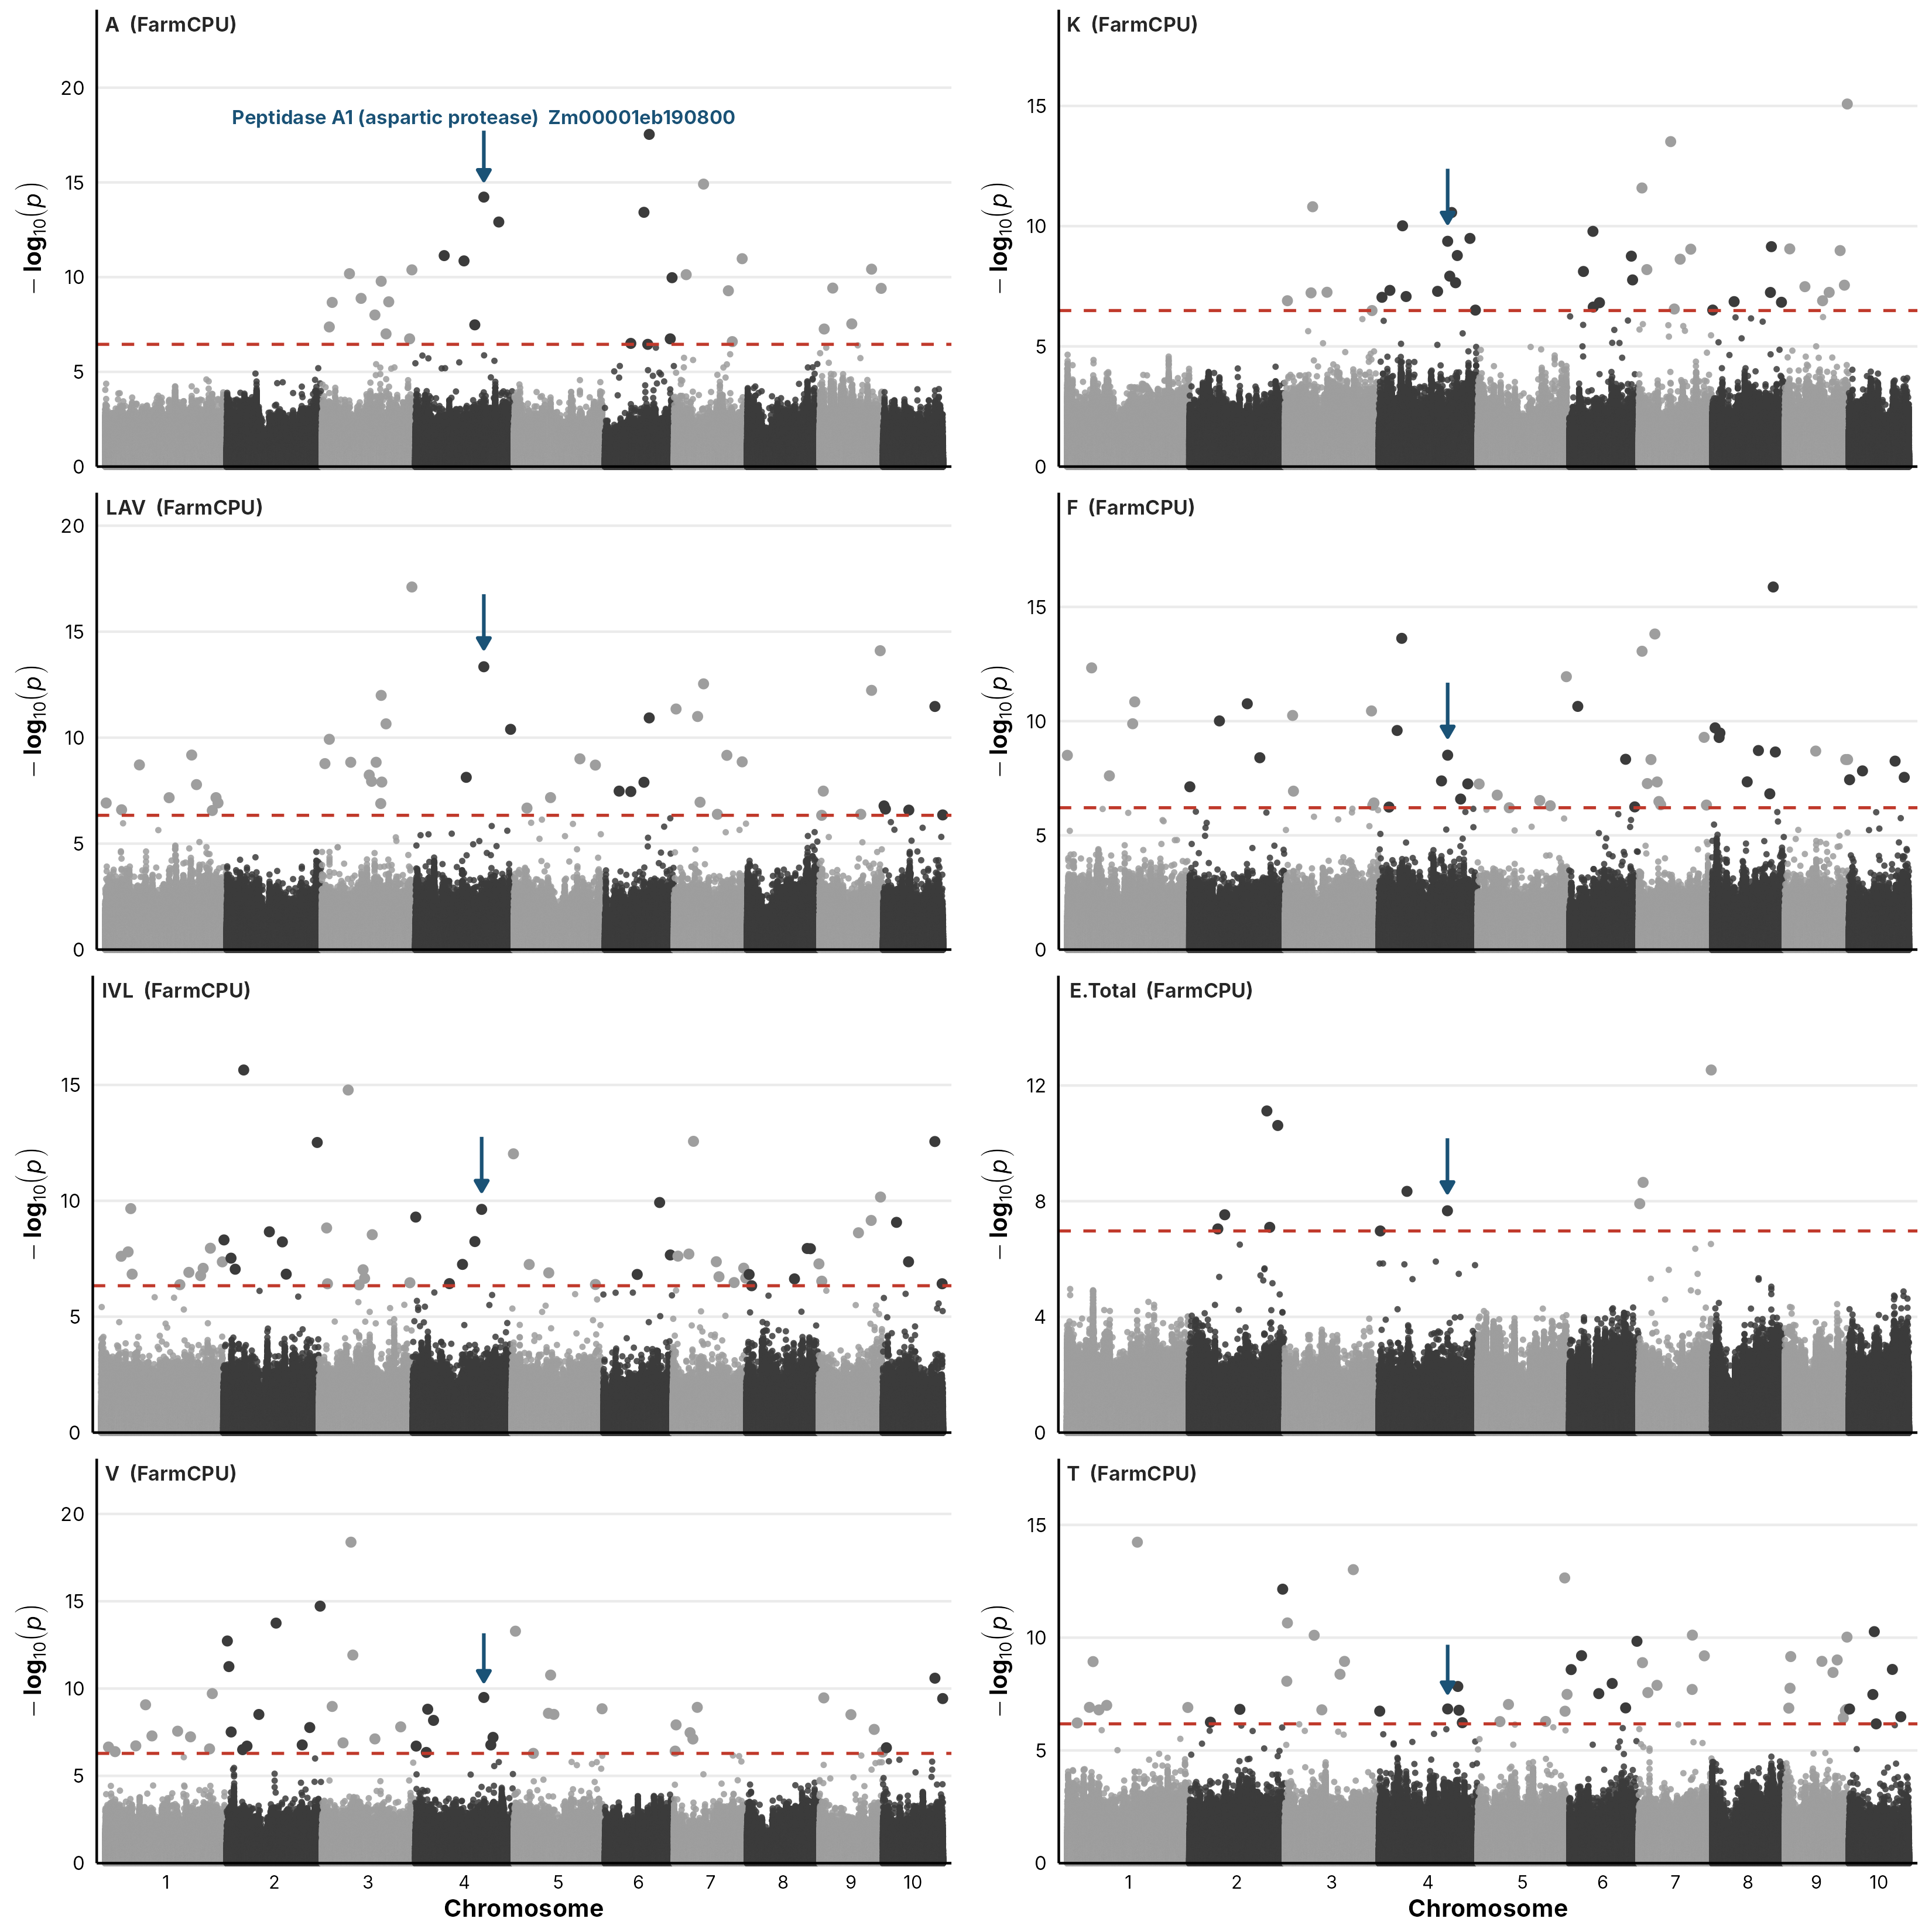
\includegraphics[width=0.82\textwidth]{final/main_figs/Fig_amino_chr4_peptidaseA1_manhattan.png}
    \caption{A locus on chromosome 4 associated with eight amino acid phenotypes lies next to a peptidase A1 (aspartic protease) gene. Manhattan plots (FarmCPU) for the eight phenotypes significant at the locus (chr4:174.55--174.57 Mb): alanine (\textit{A}), the composites \textit{LAV} and \textit{IVL}, valine (\textit{V}), lysine (\textit{K}), phenylalanine (\textit{F}), \textit{E.Total} and threonine (\textit{T}). Arrows mark the strongest SNP within 250 kb of \textit{Zm00001eb190800} (peptidase A1; chr4:174,557,846--174,559,120). Three SNPs in strong linkage disequilibrium ($r^2 = 0.92$--$0.94$; \textit{E.Total}, \textit{K}, \textit{F}, \textit{IVL}, \textit{LAV}, \textit{T}) lie 2.6--6.1 kb upstream of the gene, and a fourth (\textit{A}, \textit{V}; $P = 6.0 \times 10^{-15}$), in weak linkage disequilibrium with them ($r^2 = 0.25$--$0.27$), lies 5.9 kb downstream. All 4,177,796 SNPs are plotted at B73 RefGen\_v5 positions lifted from AGPv4; SNPs above the threshold are drawn larger. Dashed red lines indicate the 5\% Benjamini--Hochberg FDR threshold for each phenotype ($P = 6.6 \times 10^{-7}$ to $1.1 \times 10^{-7}$; $-\log_{10}$ 6.2--7.0).}
    \label{fig:amino_locus_manhattan}
\end{figure*}

\subsection{Association mapping identifies amino acid metabolism and transport candidates for abundant, heritable free amino acids}

To identify loci affecting grain amino acid composition, we scanned 78 amino acid–derived phenotypes (Supplementary Tables S1--S2), including the absolute abundance of 20 individual FAAs; six biosynthetic-family composites (IMNTDK, EHPRQ, SGC, WFY, LAV, IVL); 20 ratios to the total free pool; 25 ratios to the family composite; four ratios between amino acids (N.D, N.E, N.Q, Q.E); and three whole-pool measures (total FAA, total PBAA \citep{Shrestha2022}, and estimated nitrogen).

At a BH FDR of 5\%, we found 2,461 significant SNPs across 71 phenotypes, forming 2,152 loci and yielding 3,693 candidate genes (Supplementary Tables S6--S7). Most candidate genes were specific to one phenotype (3,002 of 3,693), while only 691 were shared by two or more phenotypes and only 193 by more than two. Because many phenotypes are composites or ratios of the same amino acids, even this sharing overstates independent overlap; at the chromosome 9 locus, for example, nine associated phenotypes resolve into three groups of SNPs that are not in linkage disequilibrium (Supplementary Fig.~\ref{fig:supp_amino_chr9_locus}). Per phenotype, the number of candidate genes was similar across families (71, 69, and 67 for aspartate, glutamate, and serine phenotypes), so family-level gene counts mainly reflect how many phenotypes each family contributes. The loci shared by the most phenotypes were not near genes annotated for amino acid biosynthesis. Three were significant for nine phenotypes each (chromosome 4 at 212.55 Mb, with no gene within 25 kb; chromosome 7 at 40.80 Mb, near a K homology domain protein, \textit{Zm00001eb306240}; and chromosome 9 at 133.93 Mb). The next, on chromosome 4 at 174.57 Mb, was significant for eight phenotypes, including five amino acids from four biosynthetic families (alanine, valine, lysine, phenylalanine, and threonine), and lies next to \textit{Zm00001eb190800}, which encodes a peptidase A1 (aspartic protease) (Fig.~\ref{fig:amino_locus_manhattan}). Full results (Manhattan plots, QQ plots, annotations) are available at \url{https://j83gk2-nirwan-tandukar.shinyapps.io/amino_gwas_app/}.

Furthermore, we investigated individual FAAs (Table~\ref{tab:amino_gwas_focus}). Lys, Asn, Asp, and Pro were the most heritable ($H^2=0.80$--$0.88$), with genomic heritability ranging from 0.40 (Pro) to 0.84 (Asp) (Supplementary Table S3). Asn, the most abundant ($H^2=0.83$, $h^2_g=0.68$), had the most loci (356 across abundance and five ratios) and candidates, including two asparagine synthetase domain genes (\textit{Zm00001eb036060}, \textit{Zm00001eb036070}; \textit{N.E}), a glutamine amidotransferase type 2 (\textit{Zm00001eb329710}; \textit{N.E}, $P=6.1\times10^{-10}$), homoserine dehydrogenase (\textit{Zm00001eb405410}; \textit{N.IMNTDK}, SNP within gene), and lysine-branch enzymes dihydrodipicolinate synthase/reductase (\textit{Zm00001eb389290}, \textit{Zm00001eb176170}). An AVT6C transporter (\textit{Zm00001eb368680}) was significant for Asn ($P=1.3\times10^{-8}$) and the Asp-family composite ($P=2.5\times10^{-11}$) in both BLINK and FarmCPU. Asparagine synthetase genes were not among the Asn candidates. In a B64 $\times$ CML14 biparental population, kernel free Asn is controlled mainly by a single QTL at \textit{ASN3} (\textit{Zm00001eb013430}), which was not detected by GWAS in this panel because no HapMap3 SNPs lie within the gene and B64 carries a 921-bp deletion in it \citep{Fitzsimmons2026KernelKitchen}. Structural variants of this kind can be missed by SNP-based association mapping.  Such structural variants can be missed by SNP-based association mapping. For lysine, the most heritable FAA ($H^2 = 0.88$, $h^2_g = 0.73$), a SNP for lysine as a fraction of the total free pool (\textit{K.Total}; $P = 2.5 \times 10^{-11}$; significant in BLINK and FarmCPU) lies in \textit{Zm00001eb277160}, an NRT1/PTR family 4.6 transporter gene. Another SNP for lysine relative to aspartate-family amino acids (\textit{K.IMNTDK}; $P = 2.8 \times 10^{-11}$) is 15~kb from \textit{Zm00001eb360480}, which encodes NADH-dependent glutamate synthase.

Pro, the second most abundant FAA, was nearly as heritable as Asn ($H^2 = 0.80$) but had a lower genomic heritability ($h^2_g = 0.40$), suggesting that the markers capture less of its variation among lines. It also had fewer loci (59). However, its ratio traits had no significant associations. One proline SNP lies within a class I glutamine amidotransferase gene (\textit{Zm00001eb217220}; $P = 2.2 \times 10^{-9}$).
% and falls in a top-5\% $F_{ST}$ window in Indian Chief (Supplementary Table S19).
Glutamine, the second most variable FAA (CV 130\%) with high genomic heritability (0.85), showed the strongest association among the amino acids in Table~\ref{tab:amino_gwas_focus} ($P = 4.9 \times 10^{-22}$, \textit{Q.E}). SNPs associated with glutamine lay within a WAT1-related (UmamiT) gene (\textit{Zm00001eb379220}; \textit{Q}, $P = 1.2 \times 10^{-11}$) and within or near a cluster of three amino acid transporter genes on chromosome 6 (\textit{Zm00001eb261470}--\textit{Zm00001eb261490}; \textit{Q.E}). Methionine, the most variable FAA (CV 180\%), had 104 loci but no trait-matched candidate gene. Its high CV likely reflects a strongly skewed distribution across lines, where the highest line had about 200 times as much methionine as the lowest (Supplementary Table S3). Thus, the most robust gene-level associations were specific to each trait. Genes involved in Asn/Asp-family metabolism and amino acid transport linked to their respective amino acids, whereas loci common to multiple phenotypes suggested roles in protein turnover rather than in single biosynthetic reactions.

%===================== TABLE 1 =====================

\begin{table*}[t]
\centering
\caption{Association mapping of the focal free amino acids (FAAs) in the Goodman--Buckler panel: the two most abundant (asparagine, proline), the most heritable (lysine, asparagine, aspartate, proline), the amide glutamine and the most variable (methionine). Median, coefficient of variation (CV), line-mean broad-sense heritability ($H^2$) and genomic heritability ($h^2_g$) are from Supplementary Table~S3. Loci: loci (Supplementary Table~S7) significant at 5\% Benjamini--Hochberg FDR for at least one phenotype reporting on the amino acid (its absolute abundance and its ratios); in parentheses, loci for the absolute trait alone. Best $P$: smallest $P$ among those phenotypes. Trait-matched candidate genes: B73 RefGen\_v5 genes within 25~kb of a significant SNP for one of those phenotypes whose annotation places them in the metabolism of the amino acid or its biosynthetic family, in amino acid or nitrogen transport, or in primary nitrogen assimilation (Methods), with their putative function; the associated phenotypes, $P$ values and SNP--gene distances are in Supplementary Table~S6.}
\label{tab:amino_gwas_focus}
\footnotesize
\setlength{\tabcolsep}{3pt}
\begin{tabularx}{\textwidth}{@{}l r r r r r r >{\raggedright\arraybackslash}X@{}}
\hline
FAA & Median & CV (\%) & $H^2$ & $h^2_g$ & Loci & Best $P$ & Trait-matched candidate genes (putative function) \\
\hline
Asparagine (N) & 3.783 & 70 & 0.83 & 0.68 & 356 (73) & $2.8\times10^{-20}$ & \textit{Zm00001eb368680} (amino acid transporter AVT6C); \textit{Zm00001eb329710} (glutamine amidotransferase type 2); \textit{Zm00001eb405410} (homoserine dehydrogenase); \textit{Zm00001eb036060} (asparagine synthetase domain); \textit{Zm00001eb036070} (asparagine synthetase domain); \textit{Zm00001eb389290} (dihydrodipicolinate synthase); \textit{Zm00001eb176170} (dihydrodipicolinate reductase) \\
Proline (P) & 3.202 & 63 & 0.80 & 0.40 & 59 (59) & $2.7\times10^{-15}$ & \textit{Zm00001eb217220} (glutamine amidotransferase) \\
Lysine (K) & 0.272 & 90 & 0.88 & 0.73 & 116 (54) & $8.3\times10^{-16}$ & \textit{Zm00001eb277160} (NRT1/PTR family 4.6); \textit{Zm00001eb360480} (glutamate synthase (NADH)); \textit{Zm00001eb352400} (WAT1-related (UmamiT)) \\
Aspartate (D) & 1.178 & 76 & 0.81 & 0.84 & 91 (20) & $3.3\times10^{-16}$ & \textit{Zm00001eb207630} (WAT1-related (UmamiT)) \\
Glutamine (Q) & 0.371 & 130 & 0.69 & 0.85 & 165 (65) & $4.9\times10^{-22}$ & \textit{Zm00001eb379220} (WAT1-related (UmamiT)); \textit{Zm00001eb261470} (amino acid transporter); \textit{Zm00001eb261480} (amino acid transporter); \textit{Zm00001eb261490} (amino acid transporter) \\
Methionine (M) & 0.047 & 180 & 0.78 & 0.46 & 104 (56) & $3.2\times10^{-17}$ & none \\
\hline
\end{tabularx}
\end{table*}

\subsection{Soil nitrogen environment GWAS of maize landraces points to candidate genes in aspartate-family and amide nitrogen metabolism}

In the Goodman--Buckler panel, the free amino acid pool of the grain was dominated by Asn and Pro, which, along with Lys and Asp, were also among the most heritable free amino acids. Association mapping identified 3,693 candidate genes, including genes involved in Asn and Asp-family metabolism and amino acid transport. Because amino acids are the main transport form of nitrogen in the plant, their metabolism may also respond to nitrogen availability in the soil. However, these inbred lines represent standing variation in temperate germplasm grown under managed fertility. We therefore turned to maize landraces collected across a soil nitrogen gradient and asked whether genetic variation associated with soil N implicates similar nitrogen-metabolism functions. Because soil N reflects the historical collection environment rather than a grain phenotype, we did not equate soil N adaptation with grain amino acid composition.

We associated the maize landrace panel \citep{RomeroNavarro2017Landraces} with total soil N at each collection site \citep{Batjes2006ISRICWISE5ArcMin}, using 0--5~cm as the primary phenotype and 5--15~cm for validation (highly correlated; $r = 0.84$ across 3,107 accessions; Fig.~\ref{fig:soilN_gwas}A--B). Because soil N is site-level (3,107 accessions but only 467 distinct values), it was largely explained by genome-wide ancestry. The genomic heritability was $\sim$1.00 and remained 0.98 after removing 50 genotype PCs (permuted $h^2 \le 0.05$; Fig.~\ref{fig:soilN_gwas}C). We therefore focused on confounding by relatedness and geography and tested it directly. Across three GWAS models, 234 SNPs were significant at 5\% FDR, while 15 appeared in at least two models and one in all three (Fig.~\ref{fig:soilN_gwas}D).

We used two tests to assess whether associations reflected soil N rather than geography or climate. First, we reran GWAS for other environmental variables (latitude, longitude, elevation, soil pH, CEC, aridity) and counted shared SNPs (Supplementary Fig.~\ref{suppfig:soilN_specificity}; Supplementary Tables~S9--S10). Only 2 of 234 soil-N SNPs were also significant for latitude/longitude/elevation, consistent with chance (0.7; $P = 0.14$). By contrast, soil N shared many SNPs with aridity (38 vs.\ 0.2 expected) and soil pH (13 vs.\ 0.1), which covary with it. Overall, 190/234 SNPs, including 14/15 multi-model SNPs, were not significant for any other variable. Second, we ranked genome-wide SNPs by genotype--environment correlation for each site variable (Supplementary Fig.~\ref{suppfig:soilN_geno_env}; Supplementary Tables~S11--S12). Soil-N GWAS SNPs were enriched in the top 1\% for geographic variables versus genome-wide SNPs (13.2\% vs.\ 1.8\%), but less so than SNPs selected by soil-N correlation alone (35.9\%; $P = 5.9 \times 10^{-15}$), indicating GWAS reduced but did not eliminate geographic signal. Of the 15 multi-model SNPs, three were associated with additional variables, including the strongest signal (S9\_151742636; $P = 2.6 \times 10^{-13}$) reflecting aridity and soil pH; five were correlated exclusively with soil N; and seven showed only weak correlations with soil N. In total, 12 SNPs detected by at least two models passed both tests (Table~\ref{tab:soilN_specific}).

Four soil-N SNPs map near genes involved in aspartate-family or amide nitrogen metabolism. S5\_22338979 lies 4.4~kb upstream of \textit{Zm00001eb220040}, an amino acid kinase-domain gene annotated with aspartate kinase activity (GO:0004072), the first step of the aspartate-derived amino acid pathway. It is the only soil-N SNP significant in all three models and is also significant at 5--15~cm. S1\_16128632 lies within \textit{Zm00001eb005710}, an $\omega$-amidase/NIT2-like CN-hydrolase \citep{Zhang2014OmegaAmidase}. Both SNPs are rare (minor allele frequencies of 0.030 and 0.016), so their associations rest on few accessions. S8\_138640842, the strongest of the 12 SNPs that passed both tests ($P = 3.5\times10^{-11}$), lies within \textit{Zm00001eb356170} (methionine S-methyltransferase); it was supported only by BLINK and FarmCPU and was inconclusive in the correlation test. At 5--15~cm, S8\_133179205 lies 0.1~kb from \textit{Zm00001eb354640} (S-adenosylmethionine synthase) and was not linked to other site variables. Thus, the soil-N GWAS in landraces, like the grain amino acid GWAS, points to aspartate-family and amide nitrogen metabolism, although these gene links are annotation-based and remain hypotheses for functional testing.

%===================== TABLE 2 =====================
\begin{table*}[ht]
  \centering
  \scriptsize
  \caption{\textbf{Soil-N SNPs detected by at least two GWAS models that passed both
  environmental specificity tests.} SNPs were FDR-significant (5\%) for soil N at 0--5~cm in at
  least two of MLM (M), BLINK (B) and FarmCPU (F); were not significant in the GWAS of latitude,
  longitude, elevation, soil pH, CEC or aridity (Supplementary Table~S10); and their genotype was
  not in the top 1\% of the genome for correlation with any of those variables
  (Supplementary Table~S11). $P$, lowest $P$ across models; 5--15~cm, also FDR-significant for
  soil N at 5--15~cm; Corr., genotype--environment correlation call: not linked, genotype
  correlates strongly with soil N and with no other variable; inconclusive, genotype correlates
  only weakly with soil N across all accessions, so the correlation test cannot judge it
  (signal detected only after the multi-locus models account for structure and other SNPs).
  Gene, nearest B73 RefGen\_v5 gene within 25~kb.}
  \label{tab:soilN_specific}
  \begin{tabular}{llrlrrllll}
  \hline
  SNP & Chr & Position & Models & MAF & $P$ & 5--15 cm & Corr. & Gene (distance) & Annotation \\
  \hline
  S8\_138640842 & 8 & 138,640,842 & BF  & 0.254 & $3.5\times10^{-11}$ & no  & inconclusive & \textit{Zm00001eb356170} (within) & Methionine S-methyltransferase \\
  S1\_87643408  & 1 &  87,643,408 & BF  & 0.356 & $2.6\times10^{-10}$ & no  & inconclusive & \textit{Zm00001eb022740} (within) & Syndetin \\
  S2\_191754648 & 2 & 191,754,648 & BF  & 0.074 & $6.2\times10^{-10}$ & no  & inconclusive & \textit{Zm00001eb100890} (within) & Uncharacterized protein \\
  S5\_22338979  & 5 &  22,338,979 & MBF & 0.030 & $1.9\times10^{-8}$  & yes & not linked   & \textit{Zm00001eb220040} (4.4 kb) & Amino acid kinase domain \\
  S8\_153826994 & 8 & 153,826,994 & BF  & 0.020 & $5.1\times10^{-8}$  & no  & inconclusive & \textit{Zm00001eb359990} (within) & Homeobox-DDT protein RLT1 \\
  S3\_54622531  & 3 &  54,622,531 & BF  & 0.050 & $6.5\times10^{-8}$  & yes & not linked   & \textit{Zm00001eb130210} (17.9 kb) & RING/FYVE/PHD zinc finger (TTL1-like) \\
  S5\_22338938  & 5 &  22,338,938 & MB  & 0.031 & $6.5\times10^{-8}$  & no  & not linked   & \textit{Zm00001eb220040} (4.3 kb) & Amino acid kinase domain \\
  S1\_16128632  & 1 &  16,128,632 & BF  & 0.016 & $2.9\times10^{-7}$  & no  & not linked   & \textit{Zm00001eb005710} (within) & $\omega$-amidase/NIT2-like CN-hydrolase \\
  S5\_53136163  & 5 &  53,136,163 & BF  & 0.221 & $5.7\times10^{-7}$  & yes & inconclusive & \textit{Zm00001eb226000} (within) & Protein kinase \\
  S6\_37926580  & 6 &  37,926,580 & BF  & 0.179 & $7.4\times10^{-7}$  & no  & inconclusive & \textit{Zm00001eb265710} (within) & HB transcription factor \\
  S1\_5543355   & 1 &   5,543,355 & BF  & 0.090 & $1.2\times10^{-6}$  & yes & inconclusive & \textit{Zm00001eb001920} (within) & Transcription repressor \\
  S2\_117202525 & 2 & 117,202,525 & BF  & 0.071 & $2.1\times10^{-6}$  & no  & not linked   & -- & No gene within 25 kb \\
  \hline
  \end{tabular}
\end{table*}

%===================== FIGURE 2 =====================
\begin{figure*}[ht!]
  \centering
  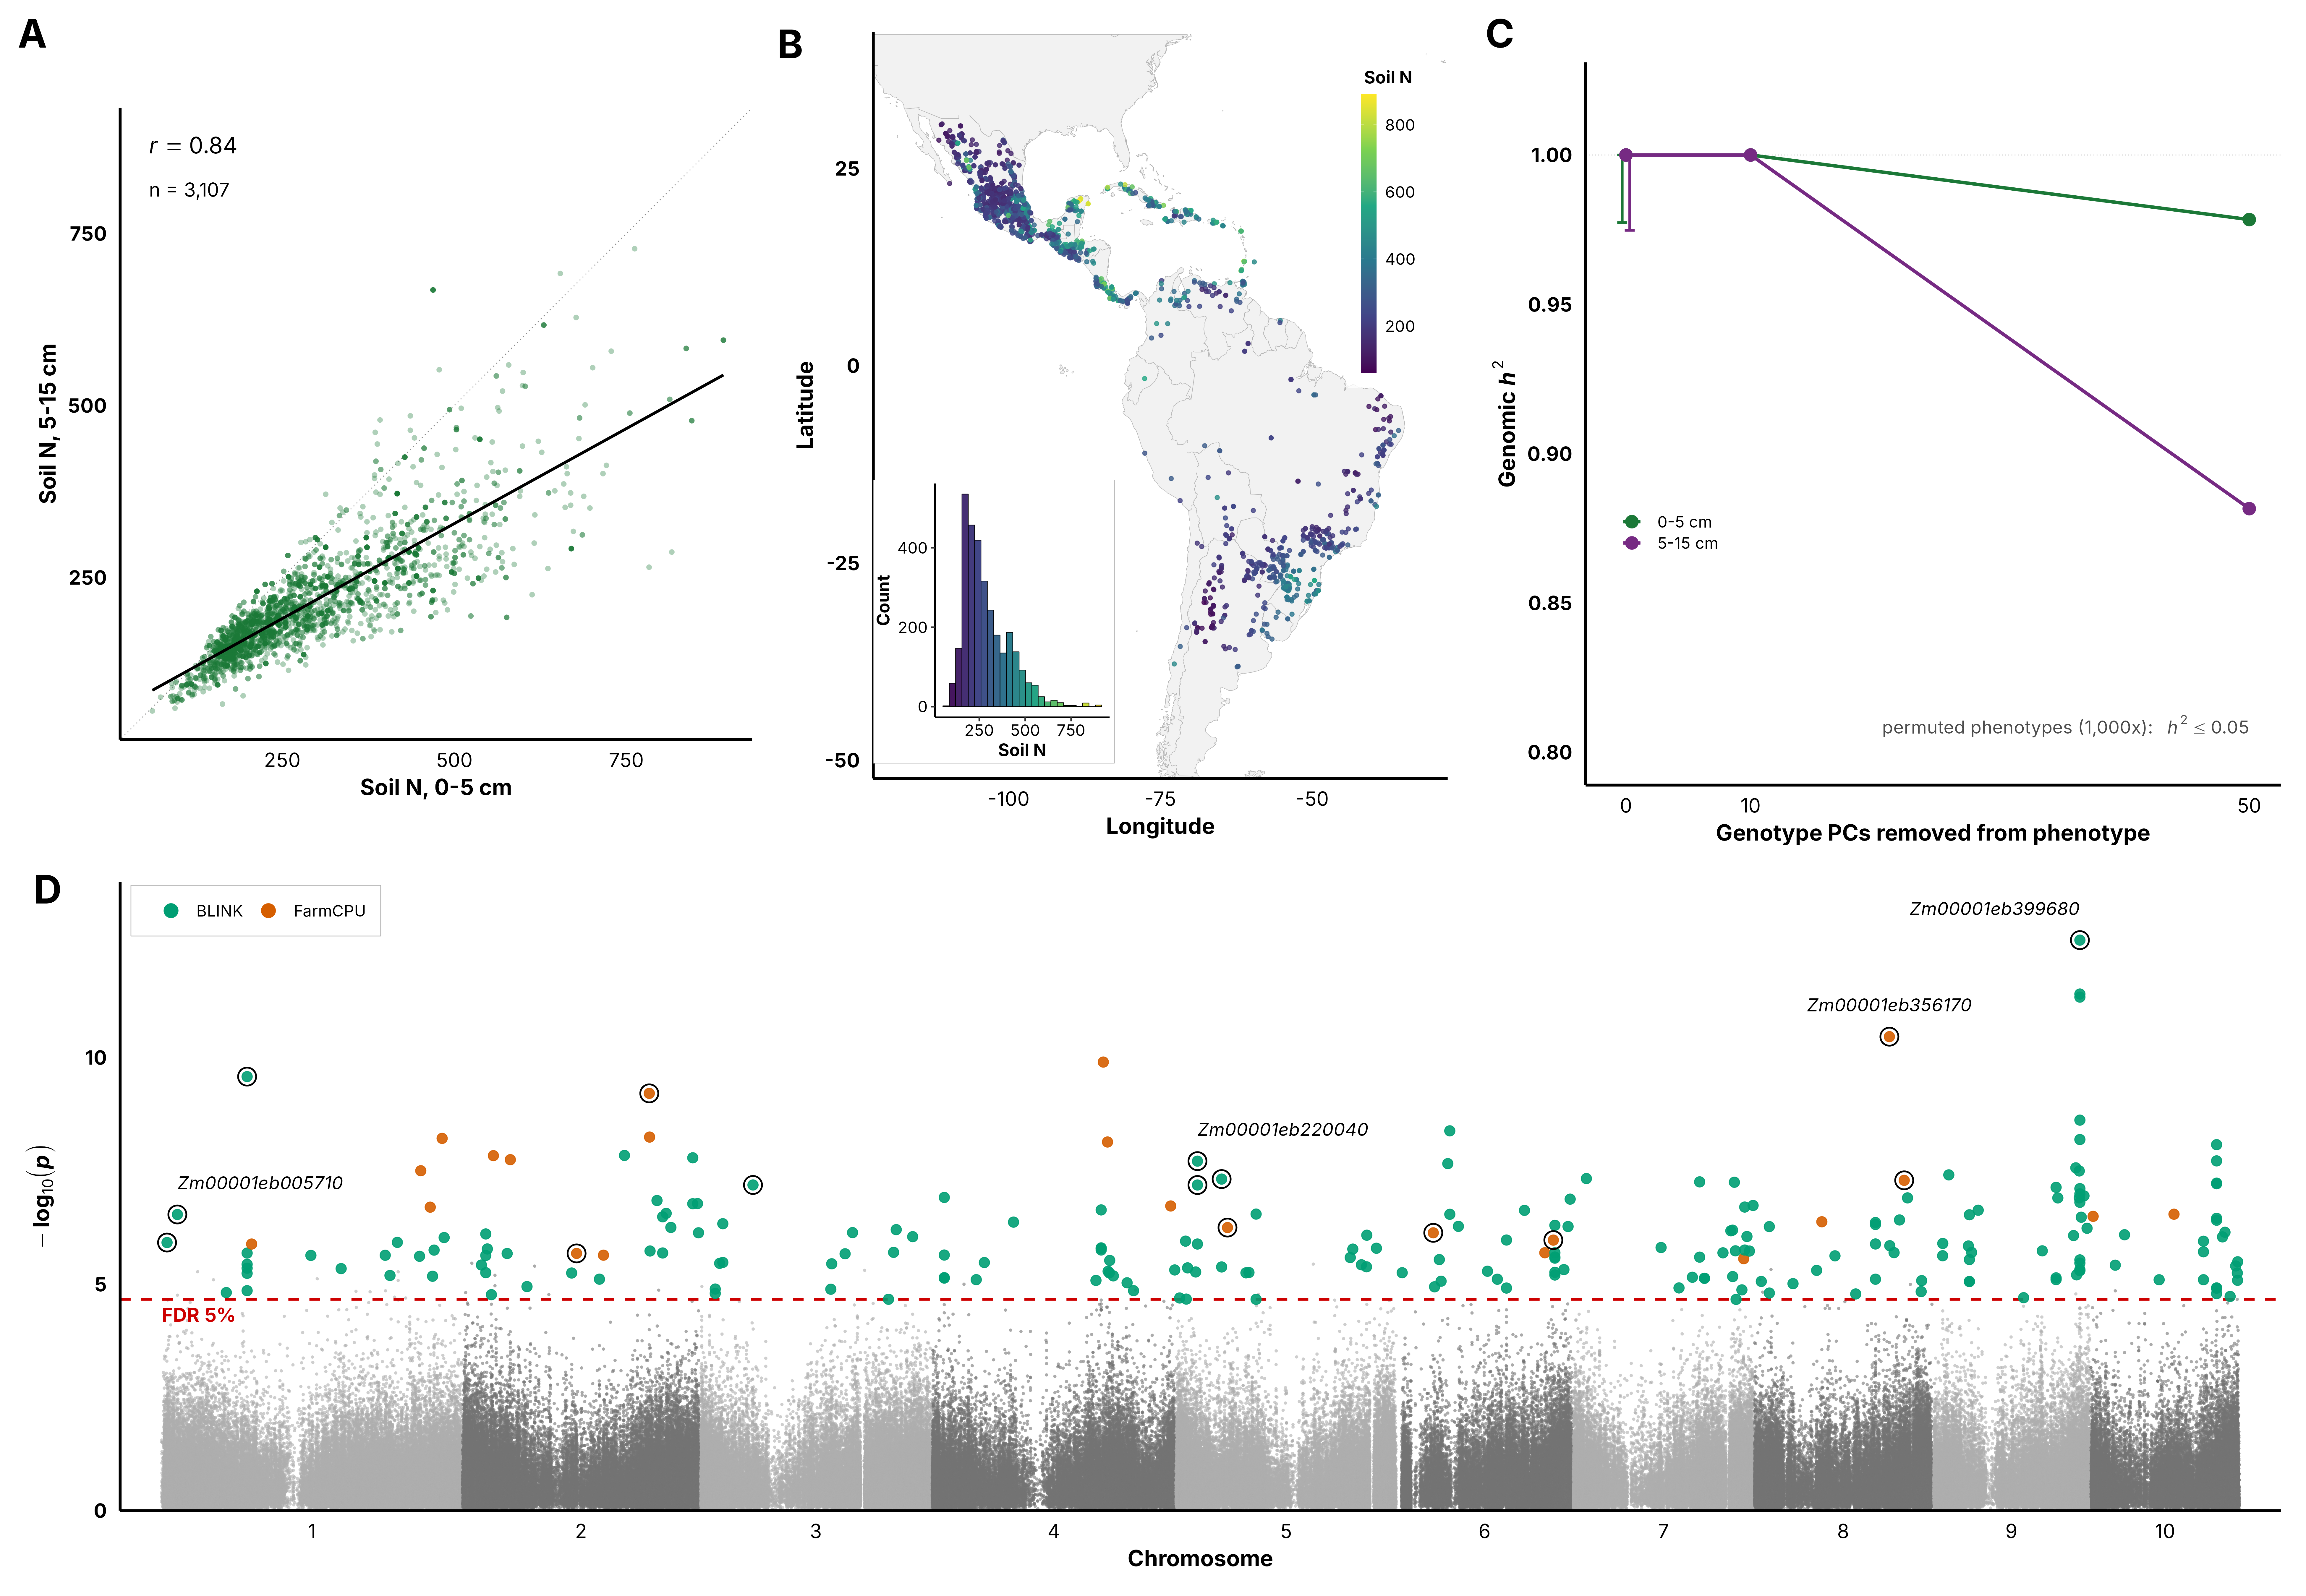
\includegraphics[width=\textwidth]{final/main_figs/Fig2_soilN.png}
  \caption{\textbf{Soil nitrogen at the collection site of 3,107 maize landraces.}
  \textbf{(A)} Soil N at 0--5\,cm vs.\ 5--15\,cm ($r = 0.84$); solid line, least-squares fit;
  dotted line, $y = x$.
  \textbf{(B)} Collection sites coloured by soil N at 0--5\,cm; inset, distribution of
  soil N across accessions.
  \textbf{(C)} Genomic heritability ($h^2$) of soil N at both depths after removing
  0, 10 and 50 genotype principal components from the phenotype; error bars, 95\% CI at
  0 PCs; permuted phenotypes (1,000$\times$) gave $h^2 \leq 0.05$.
  \textbf{(D)} Genome-wide association for soil N (0--5\,cm); all 495,755 SNPs are shown.
  Coloured points are SNPs significant at 5\% Benjamini--Hochberg FDR in at least one model
  (MLM, BLINK, FarmCPU; 3 PCs), coloured by the model with the lowest $P$; ringed points
  are significant in at least two models. The dashed red line marks the 5\% FDR threshold
  ($-\log_{10}P = 4.66$, the most lenient of the three models' thresholds).
  Candidate genes named in the text are labelled.}
  \label{fig:soilN_gwas}
\end{figure*}

\subsection{Free amino acid profiles of Indian Chief and Jarvis show population-specific remodeling of the soluble amino acid pool}

The Goodman--Buckler panel captured standing variation in grain amino acids, and landraces captured variation tied to natural soil N gradients, but neither shows how the grain amino acid pool responds to yield selection. The Indian Chief and Jarvis maize populations address this question. Both were base populations in a 14-cycle reciprocal recurrent-selection experiment for yield, and selection shifted N allocation differently \citep{Moll1994}. Under nonlimiting N, Jarvis Cycle 14 increased grain N mainly via greater grain weight, driven largely by higher post-anthesis soil N uptake, with little change in apparent stover-to-grain N remobilization. Indian Chief Cycle 14 maintained more post-anthesis stover biomass, lost less stover N after anthesis, and did not significantly increase grain N \citep{Moll1994}. Thus, grain N gains can arise from improved soil N recovery and/or altered internal N allocation during grain filling \citep{Mueller2019NUE}. Because amino acids deliver N to the kernel, we asked whether yield selection also remodeled the grain free amino acid pool, and whether populations with different N responses changed differently. We therefore view Indian Chief and Jarvis amino acid profiles as evidence of amino acid pool remodeling and N allocation differences, not direct evidence of increased N remobilization.

We compared eight pre-specified FAA metrics between Cycle~0 and Cycle~14 within each population (Fig.~\ref{fig:ic_j_faa}; Supplementary Table~S13; Methods). Indian Chief showed significant changes in total FAA and composition. Total FAA per mg increased from 1.40 (Cycle~0) to 2.46 (Cycle~14) (Wilcoxon $P = 0.0043$; BH $P = 0.017$; Fig.~\ref{fig:ic_j_faa}A), with no overlap between cycles, and FAA-derived N increased accordingly (1.75 to 2.99 per mg; BH $P = 0.017$). Pro increased from 0.320 to 0.519 of total FAA ($P = 0.016$; BH $P = 0.025$), whereas Asp decreased from 0.115 to 0.075 ($P = 0.016$; BH $P = 0.025$) and Glu from 0.140 to 0.062 ($P = 0.0068$; BH $P = 0.018$); Asn and Gln fractions were unchanged (Fig.~\ref{fig:ic_j_faa}B). Thus, Cycle 14 had higher total FAA and a shift from Asp/Glu toward Pro. When all 20 FAAs were tested together, Pro, Asp, Glu, Ile, and Val differed nominally, but none remained significant after correction (BH $P = 0.063$; Supplementary Table S14).
% The Pro increase is notable because the GWAS trait-matched proline candidate \textit{Zm00001eb217220} falls in a top-5\% $F_{ST}$ window in Indian Chief (Supplementary Table~S19).

Jarvis showed one nominal change, but the test was underpowered with only three Cycle 0 samples. The aspartate fraction increased from 0.075 (Cycle~0) to 0.137 (Cycle~14; $P = 0.019$), but it was not significant after correction (BH-adjusted $P = 0.15$). Total FAA per mg, the proline and glutamate fractions, the N-rich FAA pool, and FAA-derived N did not differ between cycles (Supplementary Table S13). The lack of corrected differences in Jarvis likely reflects limited sampling as well as FAA pool stability. A stable pool is also consistent with \citet{Moll1994}, in which the greater grain N of Jarvis Cycle 14 came mainly from greater grain weight and post-anthesis N uptake rather than from increased remobilization from the stover.

To test whether changes extended beyond the free pool, we converted FAA and PBAA abundances to amino acid derived N per mg. Protein-bound composition did not change across cycles in either population (Supplementary Fig.~\ref{fig:supp_pbaa_profiles}; Supplementary Tables~S14--S15). In Indian Chief, higher FAA derived N did not affect PBAA derived or total amino acid derived N ($P = 0.42$ for both; Supplementary Fig.~\ref{fig:supp_ic_j_aa_n_pools}; Supplementary Table~S16) because FAAs contribute <1\% of grain amino acid N, consistent with unchanged grain N in Cycle~14 \citep{Moll1994}. Jarvis showed no change in any amino acid--derived N pool. Thus, the yield selection altered the grain FAA pool in Indian Cheif, increasing total FAA and shifting composition from Asp/Glu toward Pro, while Jarvis showed no corrected change. The protein-bound pool, which contains most grain amino acid N, was unchanged in both populations. These population-specific responses align with reported selection-driven differences in N allocation \citep{Moll1994}.

\begin{figure*}[ht!]
\centering
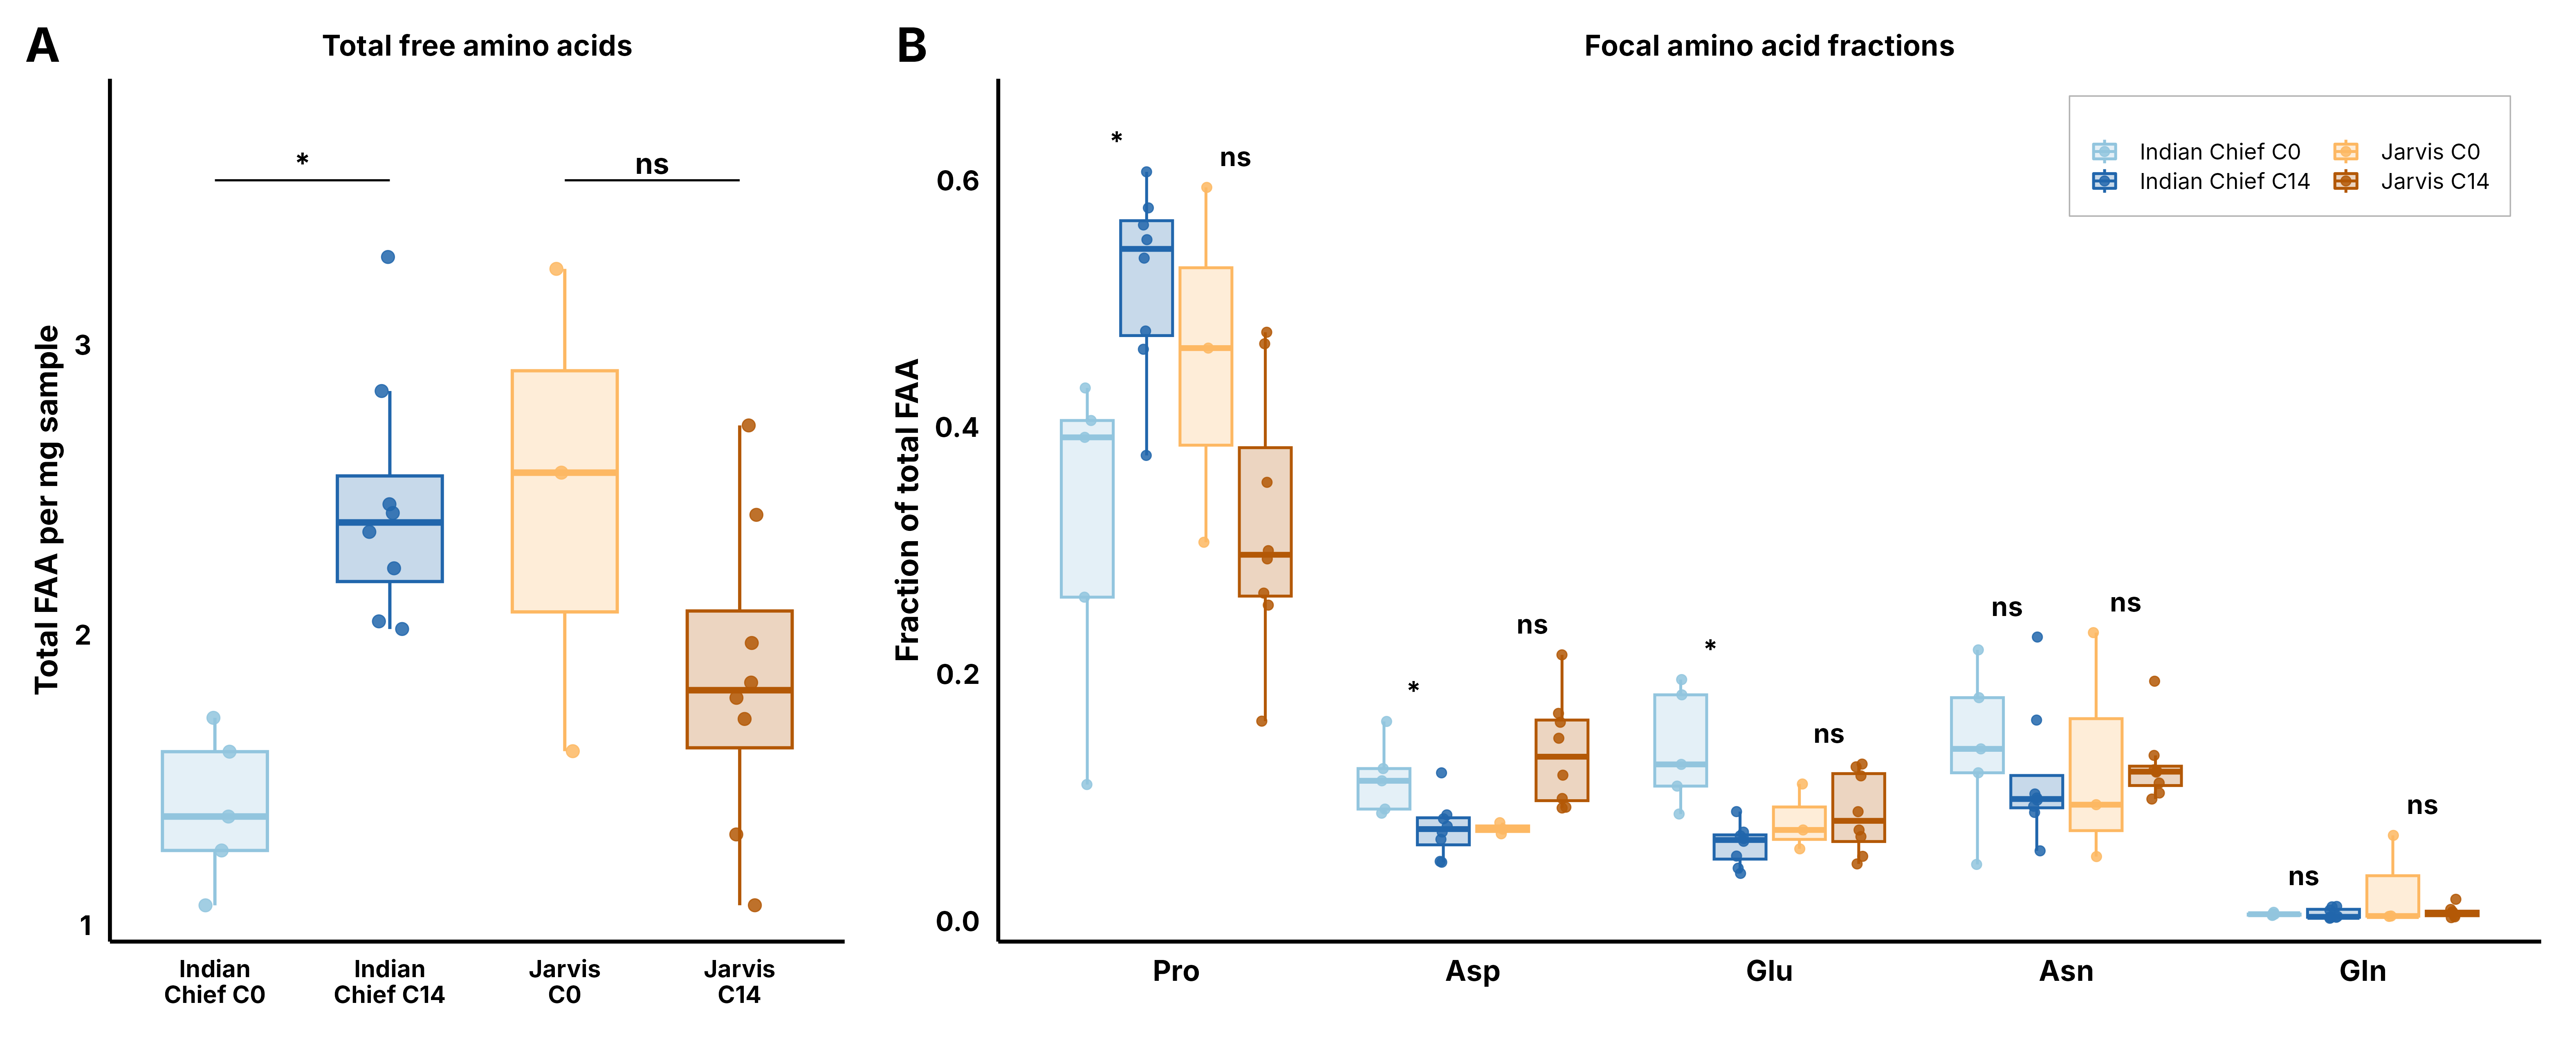
\includegraphics[width=\textwidth]{final/main_figs/Fig3_IC_J_FAA.png}
\caption{
\textbf{Free amino acid (FAA) pool and composition in Indian Chief and Jarvis before (C0) and after (C14) 14 cycles of reciprocal recurrent selection.} \textbf{(A)} Total FAA per mg sample. \textbf{(B)} Fractions of total FAA for proline, aspartate, glutamate, asparagine and glutamine. Points are biological samples, each the mean of three technical replicates (Indian Chief C0 $n = 5$, C14 $n = 8$; Jarvis C0 $n = 3$, C14 $n = 8$); boxes show the median and interquartile range. Within each population, C0 and C14 were compared with two-sided Wilcoxon rank-sum tests, and $P$ values were adjusted with the Benjamini--Hochberg method across eight pre-specified FAA metrics (Supplementary Table~S13): * adjusted $P < 0.05$; ns, not significant. In \textbf{B}, the symbol on the left of each amino acid refers to Indian Chief and the one on the right to Jarvis.
}
\label{fig:ic_j_faa}
\end{figure*}

\subsection{Skim sequencing reveals that Indian Chief and Jarvis diverged during reciprocal recurrent selection}

We skim-sequenced 379 individuals from the Indian Chief and Jarvis populations at Cycle~0 and Cycle~14 (Indian Chief 96 and 92; Jarvis 96 and 95). After filtering, 512,667 SNPs remained, mostly rare variants (median minor allele frequency 0.021), with a consistent transition/transversion ratio across chromosomes (2.88--3.08; genome-wide 2.95; Supplementary Fig.~\ref{fig:supp_seq_variant}). Mean depth at these SNPs was 0.73$\times$ (median 0.72$\times$, range 0.32--1.91$\times$) and was higher at Cycle~14 than at Cycle~0 in both populations (Indian Chief 0.61$\times$ compared to 0.88$\times$; Jarvis 0.68$\times$ compared to 0.76$\times$; Supplementary Fig.~\ref{fig:supp_seq_sample}A). Because the genotype call rate scales with depth (median 240,979 of 512,667 genotypes missing per sample; Supplementary Fig.~\ref{fig:supp_seq_sample}B), hard calls would confound depth with cycle. All population-genomic analyzes, therefore, used genotype likelihoods. The population structure was estimated from likelihoods at 82,061 of these SNPs (minor allele frequency $\ge 0.05$, one per 10~kb), and $F_{ST}$ was estimated directly from the aligned reads with ANGSD.

Unsupervised ancestry estimation (NGSadmix, $K = 2$--5) on 82,061 sites thinned to one per 10~kb separated the four population--cycle groups (Fig.~\ref{fig:ic_j_structure}A). Likelihood increased strongly to $K = 4$, where runs converged and each group formed a distinct cluster; at $K = 5$, runs disagreed and likelihood gains were small. At $K = 2$--3, Indian Chief Cycle~0 individuals were inferred as a mixture of the Jarvis Cycle~0 and Indian Chief Cycle~14 clusters, placing the ancestral Indian Chief population between Jarvis and its selected descendant. Genotype-likelihood PCA (PCAngsd) showed the same pattern (Fig.~\ref{fig:ic_j_structure}B): PC1 (14.3\%) separated Indian Chief Cycle~14 from Jarvis Cycle~14, with both Cycle~0 groups near the centre, and PC2 (6.7\%) separated Cycle~14 from Cycle~0. Overall, the populations, initially less differentiated at Cycle~0, diverged in opposite directions over 14 cycles.

Genetic differentiation confirmed divergence between the populations. $F_{ST}$ (from genotype likelihoods) between Indian Chief and Jarvis nearly doubled from 0.111 at Cycle~0 to 0.211 at Cycle~14, increasing across all ten chromosomes (Cycle~0, 0.079--0.134; Cycle~14, 0.169--0.245; Fig.~\ref{fig:ic_j_structure}C). Because Cycle~14 had deeper sequencing, which should improve allele-frequency estimates and if anything reduce $F_{ST}$, the increase is unlikely to be a depth artifact. This divergence is expected under reciprocal recurrent selection, which favors complementary rather than shared alleles \citep{Comstock1949RRS}, and is reinforced by drift in small, separately maintained populations. Thus, over 14 cycles, Indian Chief and Jarvis remained distinct while becoming more differentiated from each other and from their ancestral generations.

%===================== FIGURE 4 =====================
\begin{figure*}[ht!]
    \centering
    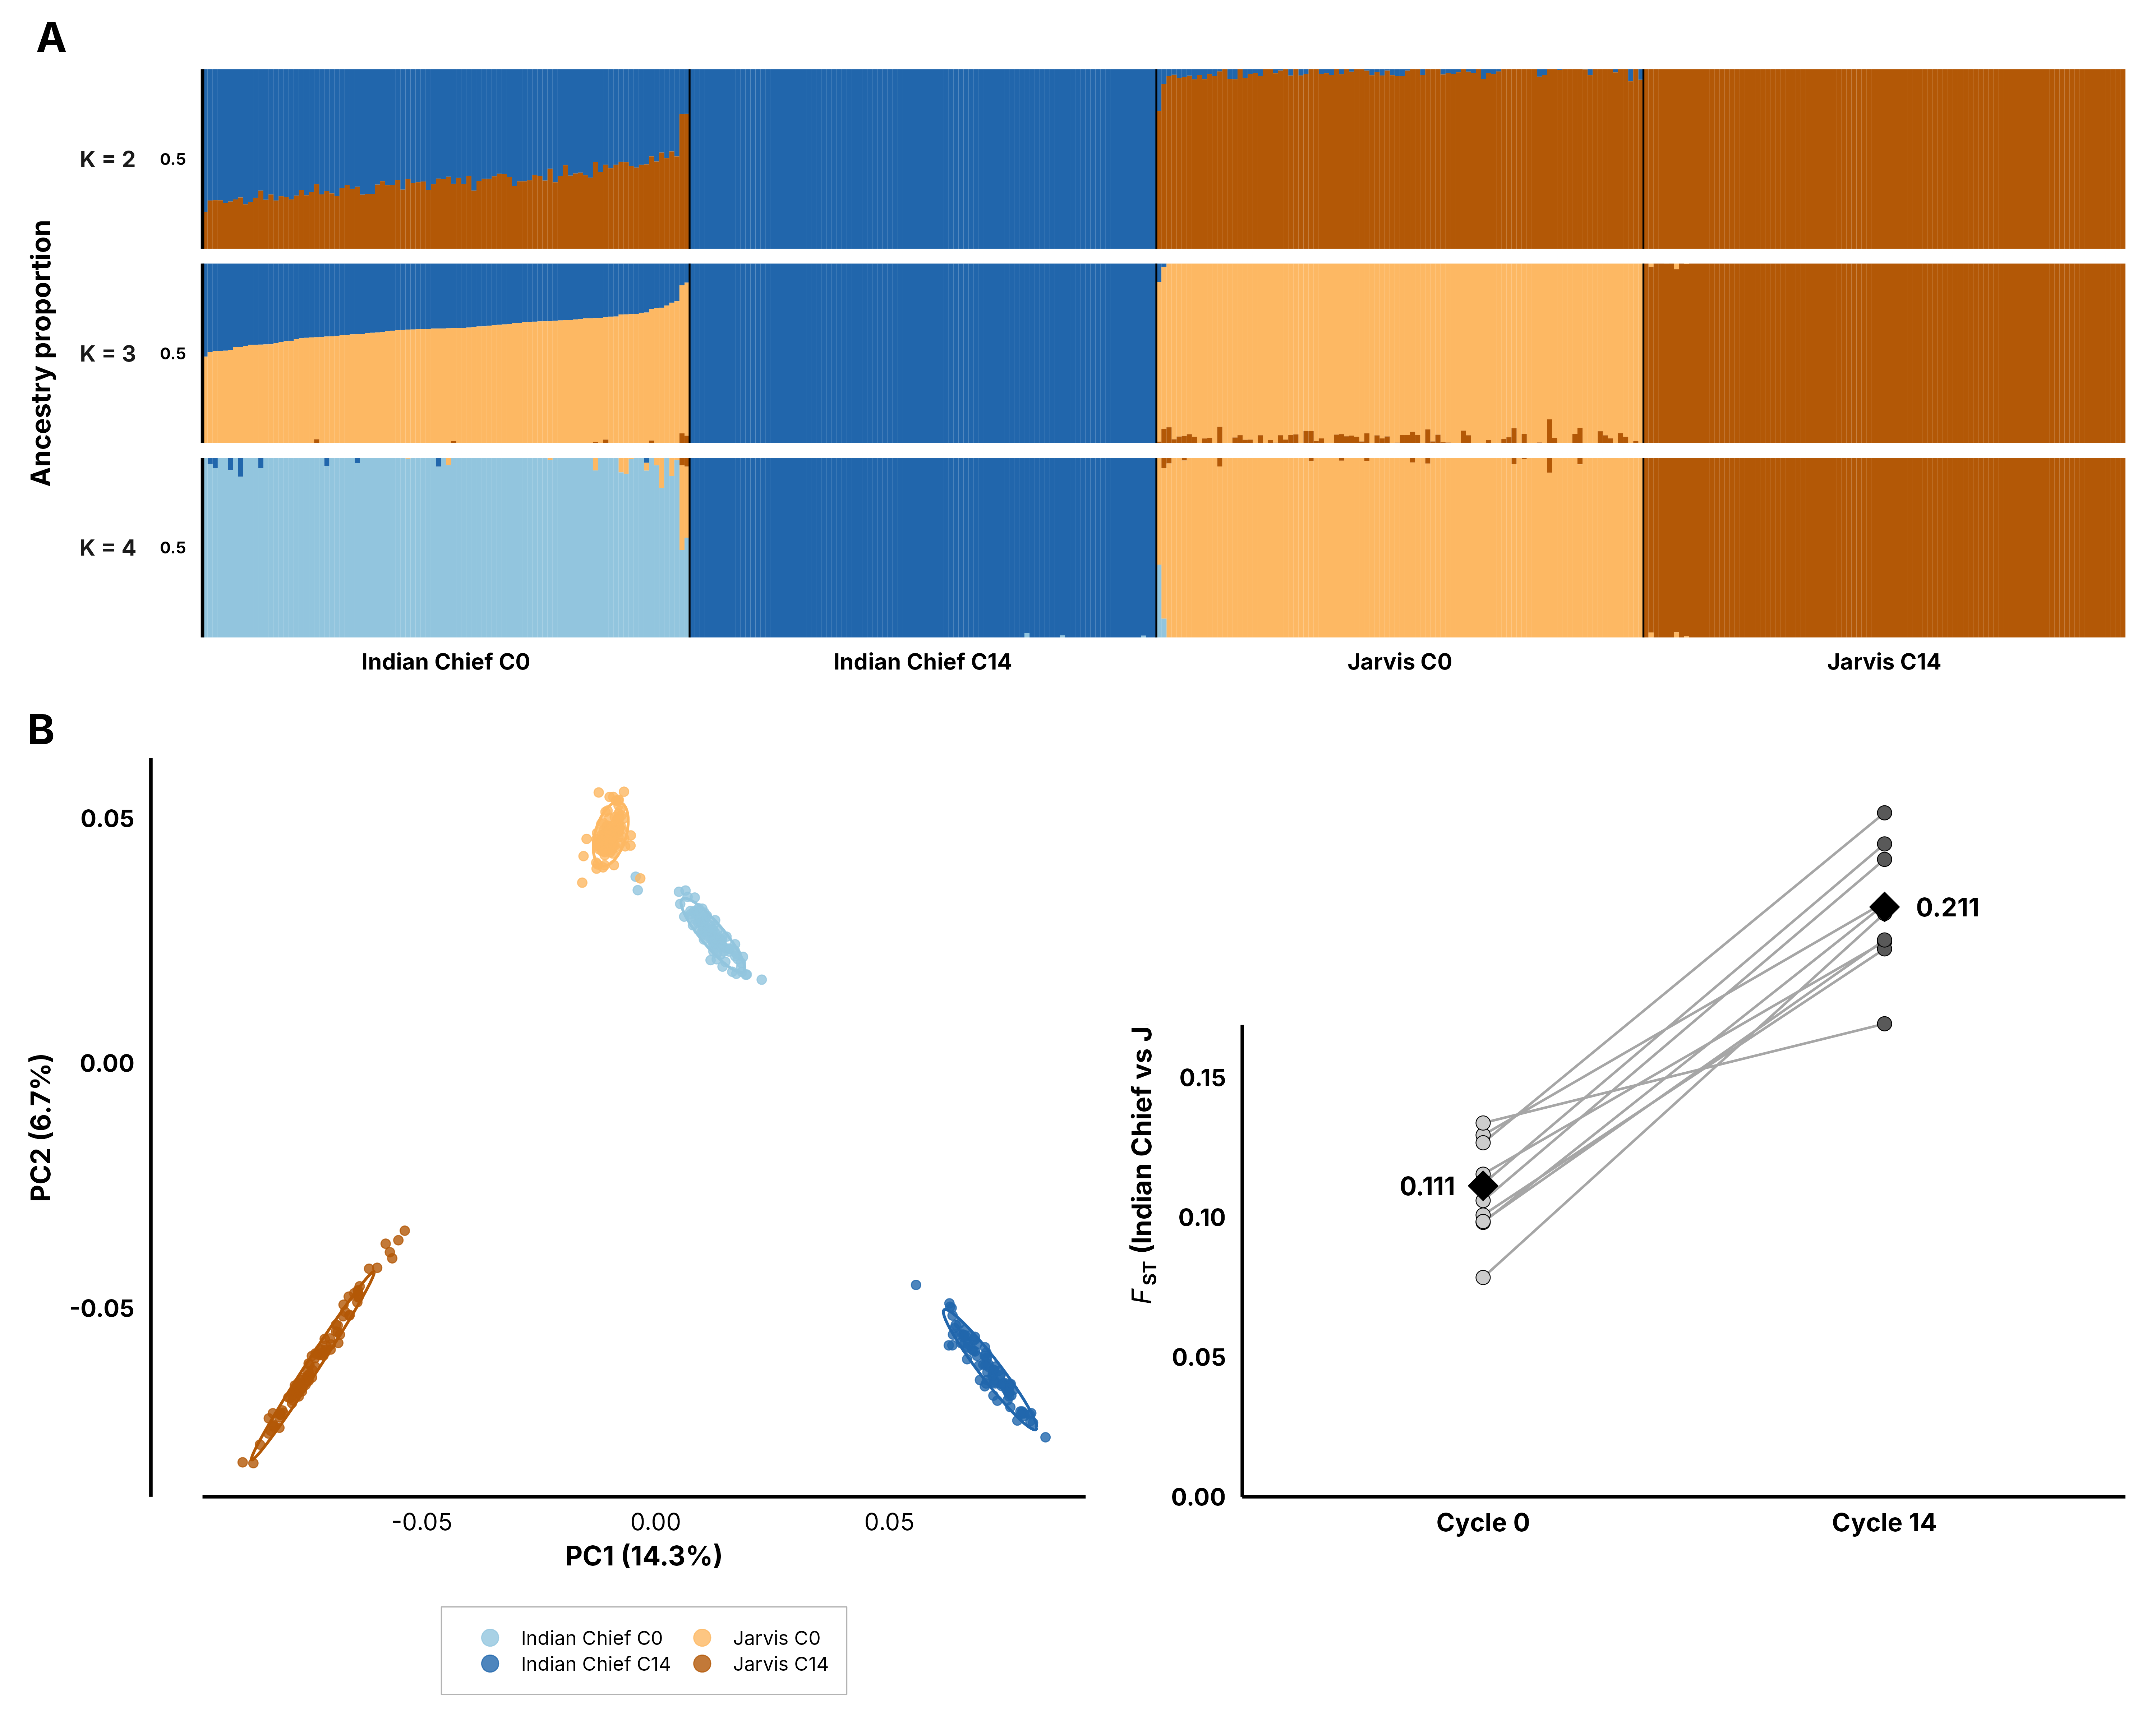
\includegraphics[width=\textwidth]{final/main_figs/Fig4_IC_J_structure.png}
    \caption{\textbf{Indian Chief and Jarvis diverged during 14 cycles of reciprocal recurrent selection.} All panels use genotype likelihoods from skim sequencing of 379 individuals (Indian Chief Cycle~0, $n = 96$; Cycle~14, $n = 92$; Jarvis Cycle~0, $n = 96$; Cycle~14, $n = 95$), because Cycle~14 was sequenced more deeply than Cycle~0. \textbf{(A)} Unsupervised ancestry proportions (NGSadmix) for $K = 2$--4 from 82,061 SNPs thinned to one per 10~kb; each bar is one individual, and each cluster is coloured by the group with the highest mean membership. $K = 4$ is the largest $K$ at which independent runs converged. \textbf{(B)} Principal component analysis of the genotype-likelihood covariance matrix (PCAngsd) on the same sites; ellipses enclose 90\% of each group. Individuals with lower depth carry less information and lie closer to the centre of their group. \textbf{(C)} Hudson $F_{ST}$ between Indian Chief and Jarvis at Cycle~0 and Cycle~14, estimated from the joint site-frequency spectrum of each pair; grey lines connect the same chromosome and black diamonds give the genome-wide value.}
    \label{fig:ic_j_structure}
\end{figure*}

\subsection{$F_{ST}$ scans identify population-specific candidate regions in Indian Chief and Jarvis}

Before scanning for selection, we asked how much of the allele-frequency change between cycles could be explained by genetic drift. In the reciprocal recurrent selection program, each cycle was formed by intermating the self-pollinated progenies of the 20 best plants per population \citep{MollStuber1971}, which implies an effective population size ($N_e$) of at most 20 per cycle. Genome-wide mean $F_{ST}$ between Cycle~0 and Cycle~14 was 0.095 in Indian Chief and 0.114 in Jarvis, values reproduced by neutral Wright--Fisher simulations at $N_e \approx 30$ and $N_e \approx 26$ per cycle, respectively (Supplementary Fig.~\ref{fig:supp_ne_drift}). Although slightly above the design-based expectation, these estimates indicate that most genome-wide change between cycles is consistent with drift in small populations. A similar conclusion was reached for the Iowa BSSS and BSCB1 reciprocal recurrent selection populations, where linked drift simulations from founder haplotypes explained most of the loss of diversity and few regions deviated from drift or were shared between populations \citep{Gerke2015DriftRRS}. At this $N_e$, drift moves long linked regions together, so individual outlier regions cannot be formally distinguished from drift. We therefore treat the scans below as exploratory.

We scanned each population for the regions with the largest allele-frequency change between Cycle~0 and Cycle~14 using $F_{ST}$ summarized in spline-defined windows (2,162 windows in Indian Chief and 2,151 in Jarvis; median length 500~kb). We retained the top 5\% of windows ($F_{ST} \ge 0.157$ in Indian Chief and $\ge 0.178$ in Jarvis; 109 and 108 windows), which contained 2,001 and 1,179 genes, respectively (Fig.~\ref{fig:ic_j_fst}; Supplementary Tables~S17--S20). Candidate regions were largely population-specific: only five regions (2.5~Mb; 73 genes) were in the top 5\% in both populations, no more than expected by chance ($P = 0.80$; Fig.~\ref{fig:ic_j_fst}), so the two populations show no evidence of shared targets of differentiation. Likewise, 192 of the 2,152 Goodman--Buckler amino acid GWAS loci (8.9\%) fell in a top-5\% window of either population, the same proportion as the genome covered by these windows (8.9\%; $P = 0.52$). Thus, the $F_{ST}$ scans and the amino acid GWAS do not converge on the same genomic regions beyond chance.

Each candidate set contains more than 1,000 genes, so genes from almost any metabolic pathway are expected to be present by chance. We therefore focused on genes in the pathways highlighted by the amino acid and soil-N GWAS (Asp-family and Glu/Gln metabolism, amino acid and N transport, and protein turnover) and describe them as annotations of interest rather than as evidence that a given pathway was selected; whether any pathway recurs across analyzes more than expected is tested in the next section. In Indian Chief, candidate regions included genes of Asp-family amino acid metabolism, \textit{Zm00001eb214360} (aspartate-semialdehyde dehydrogenase) and \textit{Zm00001eb294790} (threonine synthase), and genes of Glu/Gln interconversion, including a glutamate dehydrogenase (\textit{Zm00001eb060520}), an amino acid dehydrogenase (\textit{Zm00001eb162300}), a glutamine synthetase domain-containing protein (\textit{Zm00001eb162900}), and a glutamine amidotransferase domain-containing protein (\textit{Zm00001eb217220}), which also contains a significant SNP for proline in the Goodman--Buckler GWAS (Table~\ref{tab:amino_gwas_focus}). Candidate regions also contained genes involved in N transport and protein turnover: the senescence-specific cysteine protease \textit{SAG39} (\textit{Zm00001eb214780}) and an ammonium transporter (\textit{Zm00001eb214890}), which lie in the same window on chromosome~5; an NRT1/PTR-family transporter (\textit{Zm00001eb287950}) and the autophagy-related gene \textit{ATG18g} (\textit{Zm00001eb287690}), which share a window on chromosome~6; and two further autophagy-related genes (\textit{Zm00001eb352300} and \textit{Zm00001eb372060}). These annotations are compatible with the Indian Chief FAA phenotype, in which total FAA and the Pro fraction increased while the Asp and Glu fractions decreased from Cycle~0 to Cycle~14, but they do not establish that these genes underlie it.

In Jarvis, candidate regions included two genes of aspartate metabolism: \textit{Zm00001eb094670}, annotated as aspartate kinase, which catalyzes the first committed step of the Asp-family pathway leading to lysine, threonine, methionine, and isoleucine, and an aspartate aminotransferase (\textit{Zm00001eb152450}, GOT1/THP3). These genes are of interest because the Asp fraction was the only FAA trait that changed in Jarvis, increasing nominally from Cycle~0 to Cycle~14. Jarvis candidate regions also contained two amino acid transporter genes (\textit{Zm00001eb132750}, an amino acid transporter transmembrane domain-containing protein, and \textit{Zm00001eb159580}, a putative GABA transporter), NPL4-like protein~1 (\textit{Zm00001eb146560}), which acts in ubiquitin-dependent protein degradation, and two glutaredoxins (\textit{Zm00001eb131830} and \textit{Zm00001eb131840}). As in Indian Chief, these candidates point to amino acid metabolism, transport, and protein turnover as processes worth testing, but they remain hypotheses because drift alone can produce candidate regions of this size.

%===================== FIGURE 5 =====================
\begin{figure*}[ht!]
    \centering
    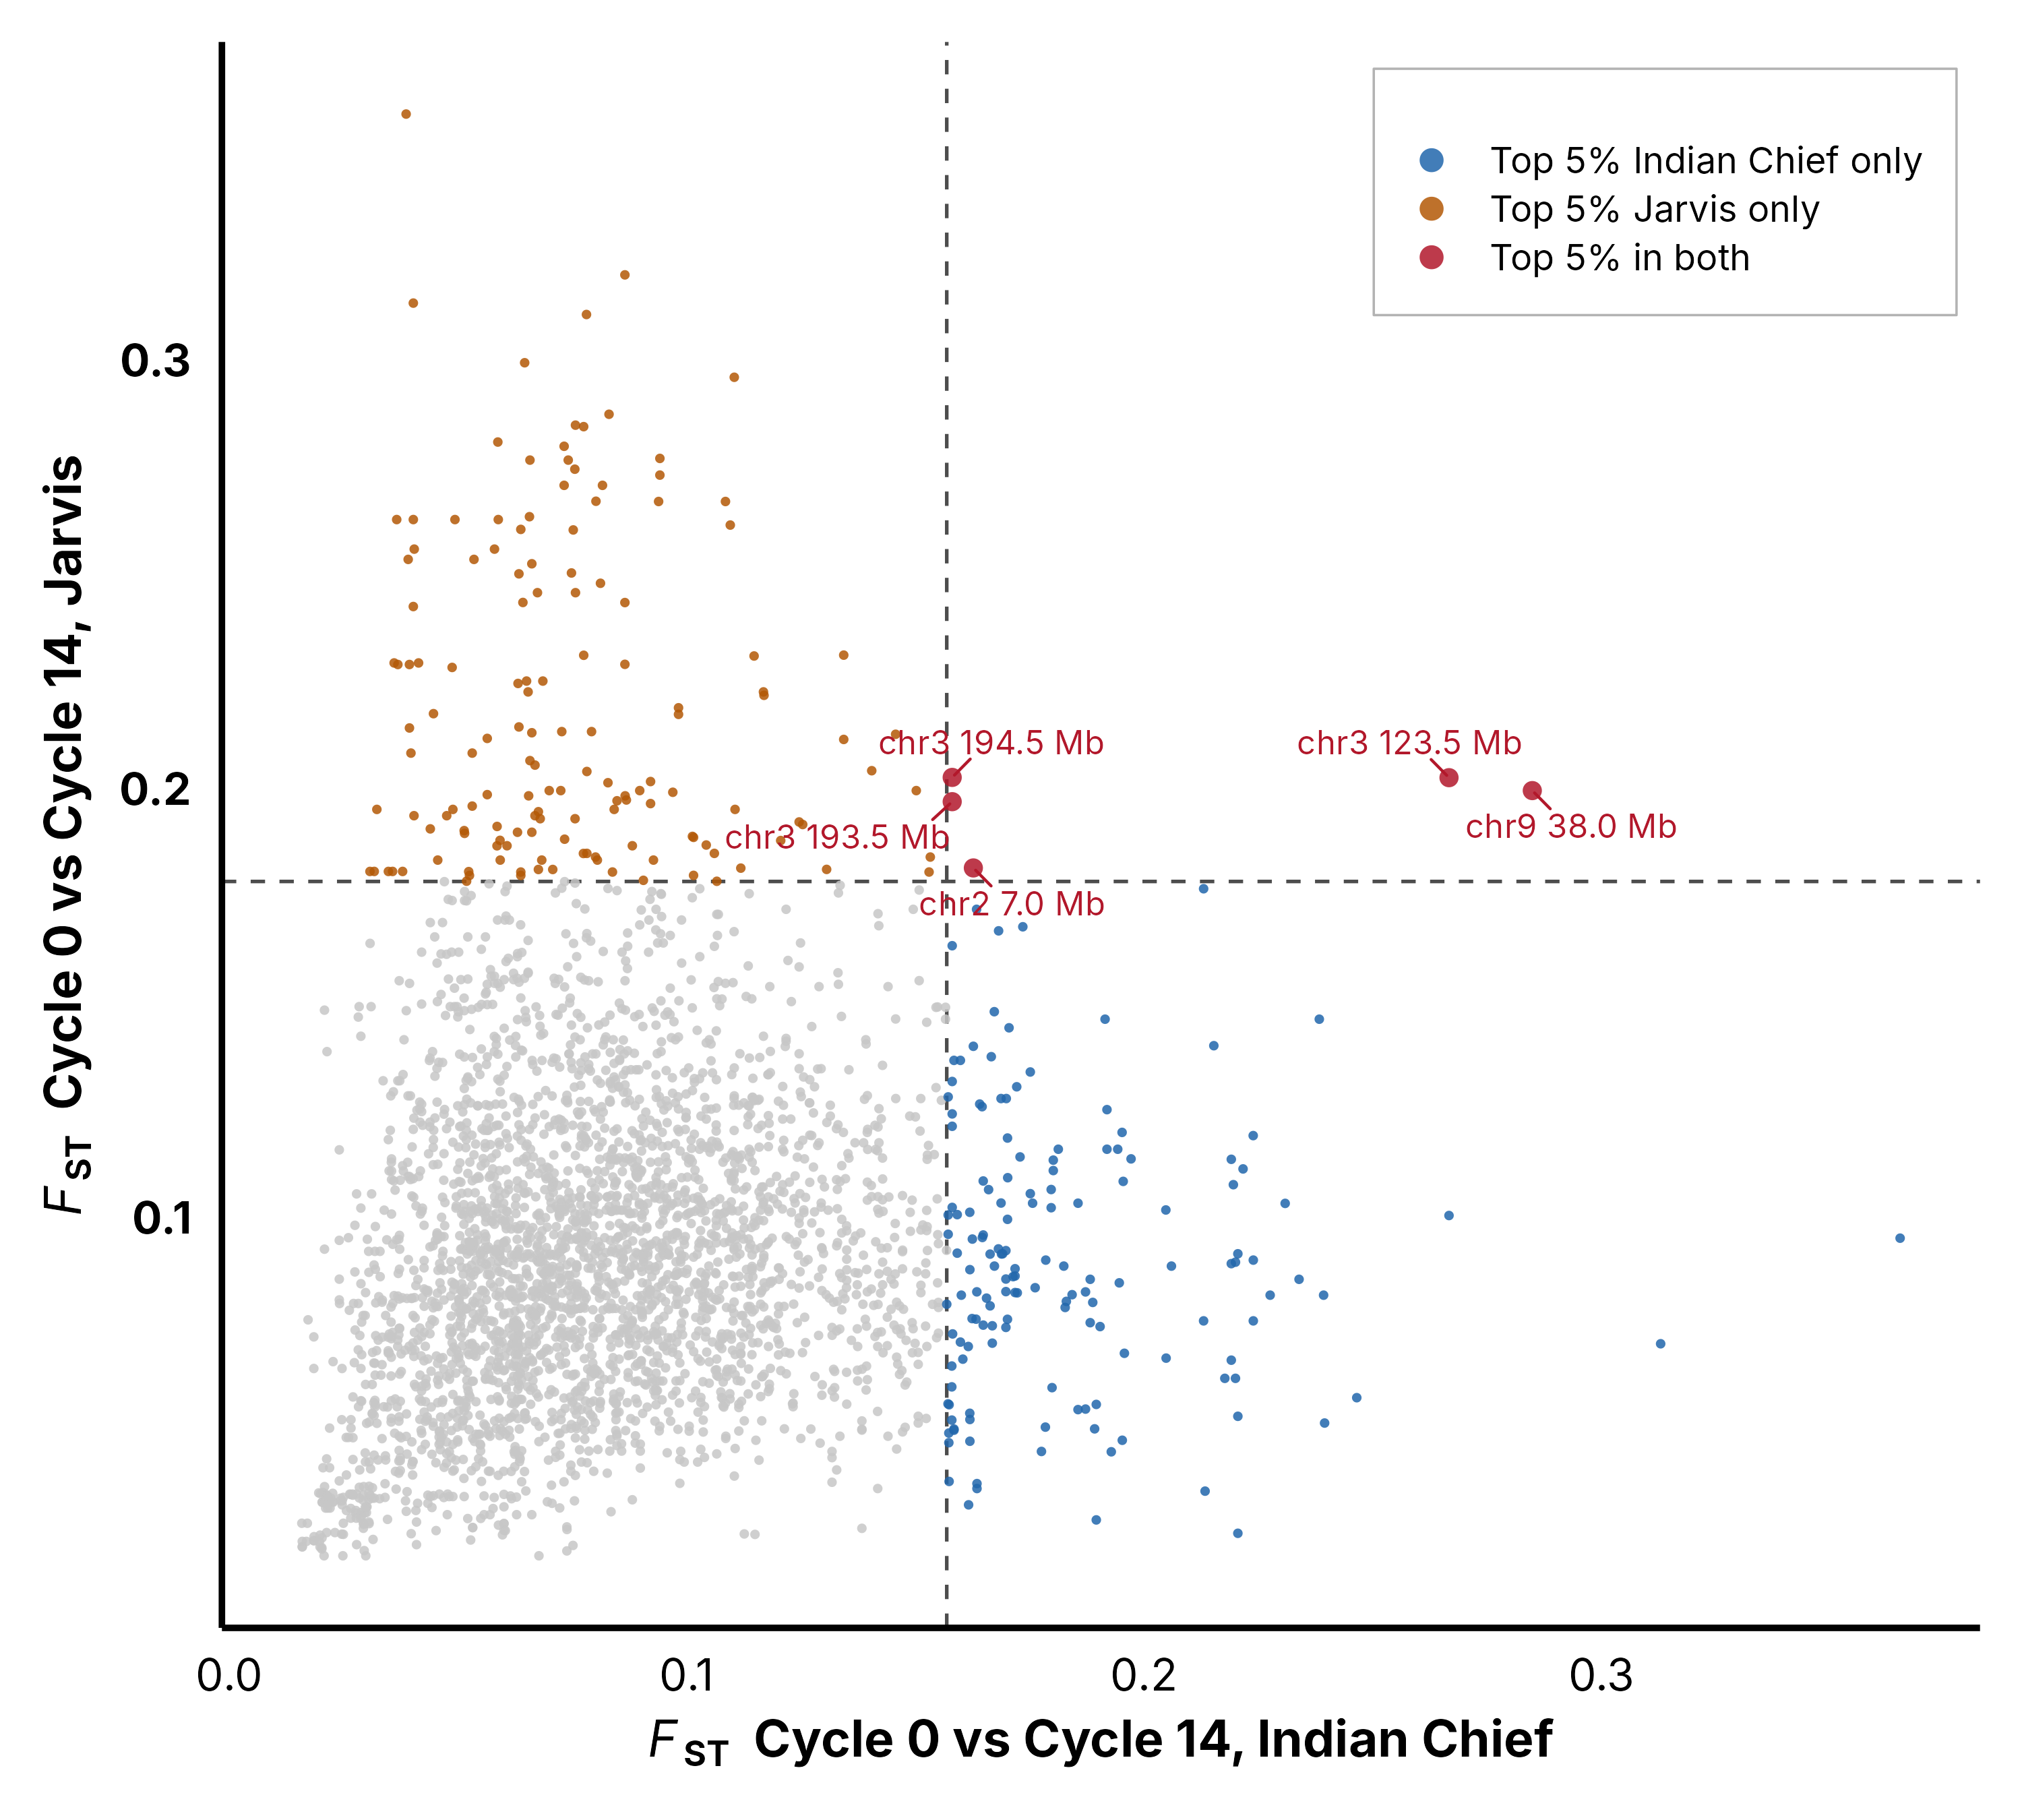
\includegraphics[width=0.75\textwidth]{final/main_figs/Fig5_IC_J_Fst_scan.png}
    \caption{\textbf{Candidate regions of differentiation between Cycle~0 and Cycle~14 are largely population-specific.} $F_{ST}$ between Cycle~0 and Cycle~14 in Indian Chief ($x$-axis) and Jarvis ($y$-axis), estimated from genotype likelihoods (ANGSD/\texttt{realSFS}) and summarized in spline-defined windows (GenWin). Because window boundaries differ between the two populations, each point is a genomic segment bounded by the window boundaries of either population, and carries the $F_{ST}$ of the Indian Chief and Jarvis windows that contain it. Dashed lines mark the top 5\% of windows in each population ($F_{ST} \geq 0.157$ in Indian Chief and $\geq 0.178$ in Jarvis). Blue and orange, top 5\% in one population only; red, top 5\% in both, labelled with chromosome and position (B73 RefGen\_v5). The overlap between populations (2.5~Mb) was no greater than expected from 10,000 circular shifts of the Jarvis scan (mean 4.4~Mb; $P = 0.80$). Top-5\% windows are empirical outliers, not significance thresholds: with $N_e \approx 25$--30 (Supplementary Fig.~\ref{fig:supp_ne_drift}), drift alone can produce windows in this range.}
    \label{fig:ic_j_fst}
\end{figure*}

\subsection{The aspartate-to-homoserine pathway recurs across the three populations}

To test whether the three populations implicate the same metabolic pathways, we asked whether any CornCyc pathway contained candidate genes from more of four analyses (amino acid GWAS, soil-N GWAS, Indian Chief, and Jarvis $F_{ST}$ scans) than expected by chance. We represented each candidate set by genomic intervals and generated a null distribution by randomly shifting intervals along the genome while preserving number, size, and clustering (20,000 permutations; Methods). Among 468 pathways, L-homoserine biosynthesis was the only one hit in all four analyses and was least likely by chance ($P = 0.0012$; Fig.~\ref{fig:pathway_recurrence}). Each analysis implicated a different enzyme: homoserine dehydrogenase (\textit{Zm00001eb405410}), an aspartate kinase isozyme (\textit{Zm00001eb220040}), aspartate-semialdehyde dehydrogenase (\textit{Zm00001eb214360}), and aspartate kinase (\textit{Zm00001eb094670}). L-lysine biosynthesis VI also recurred in all four analyses ($P = 0.0074$) via the same genes because it shares the aspartate kinase and aspartate-semialdehyde dehydrogenase steps. Other top pathways were small phytoalexin and lipid pathways hit by two or three analyses ($P = 0.003$--0.03). L-homoserine biosynthesis was not significant after correction across 468 pathways, so we treat it as suggestive. Overall, despite no shared loci, all three populations converge on the aspartate-derived amino acid pathway, specifically the conversion of aspartate to homoserine.

\begin{figure*}[ht!]
  \centering
  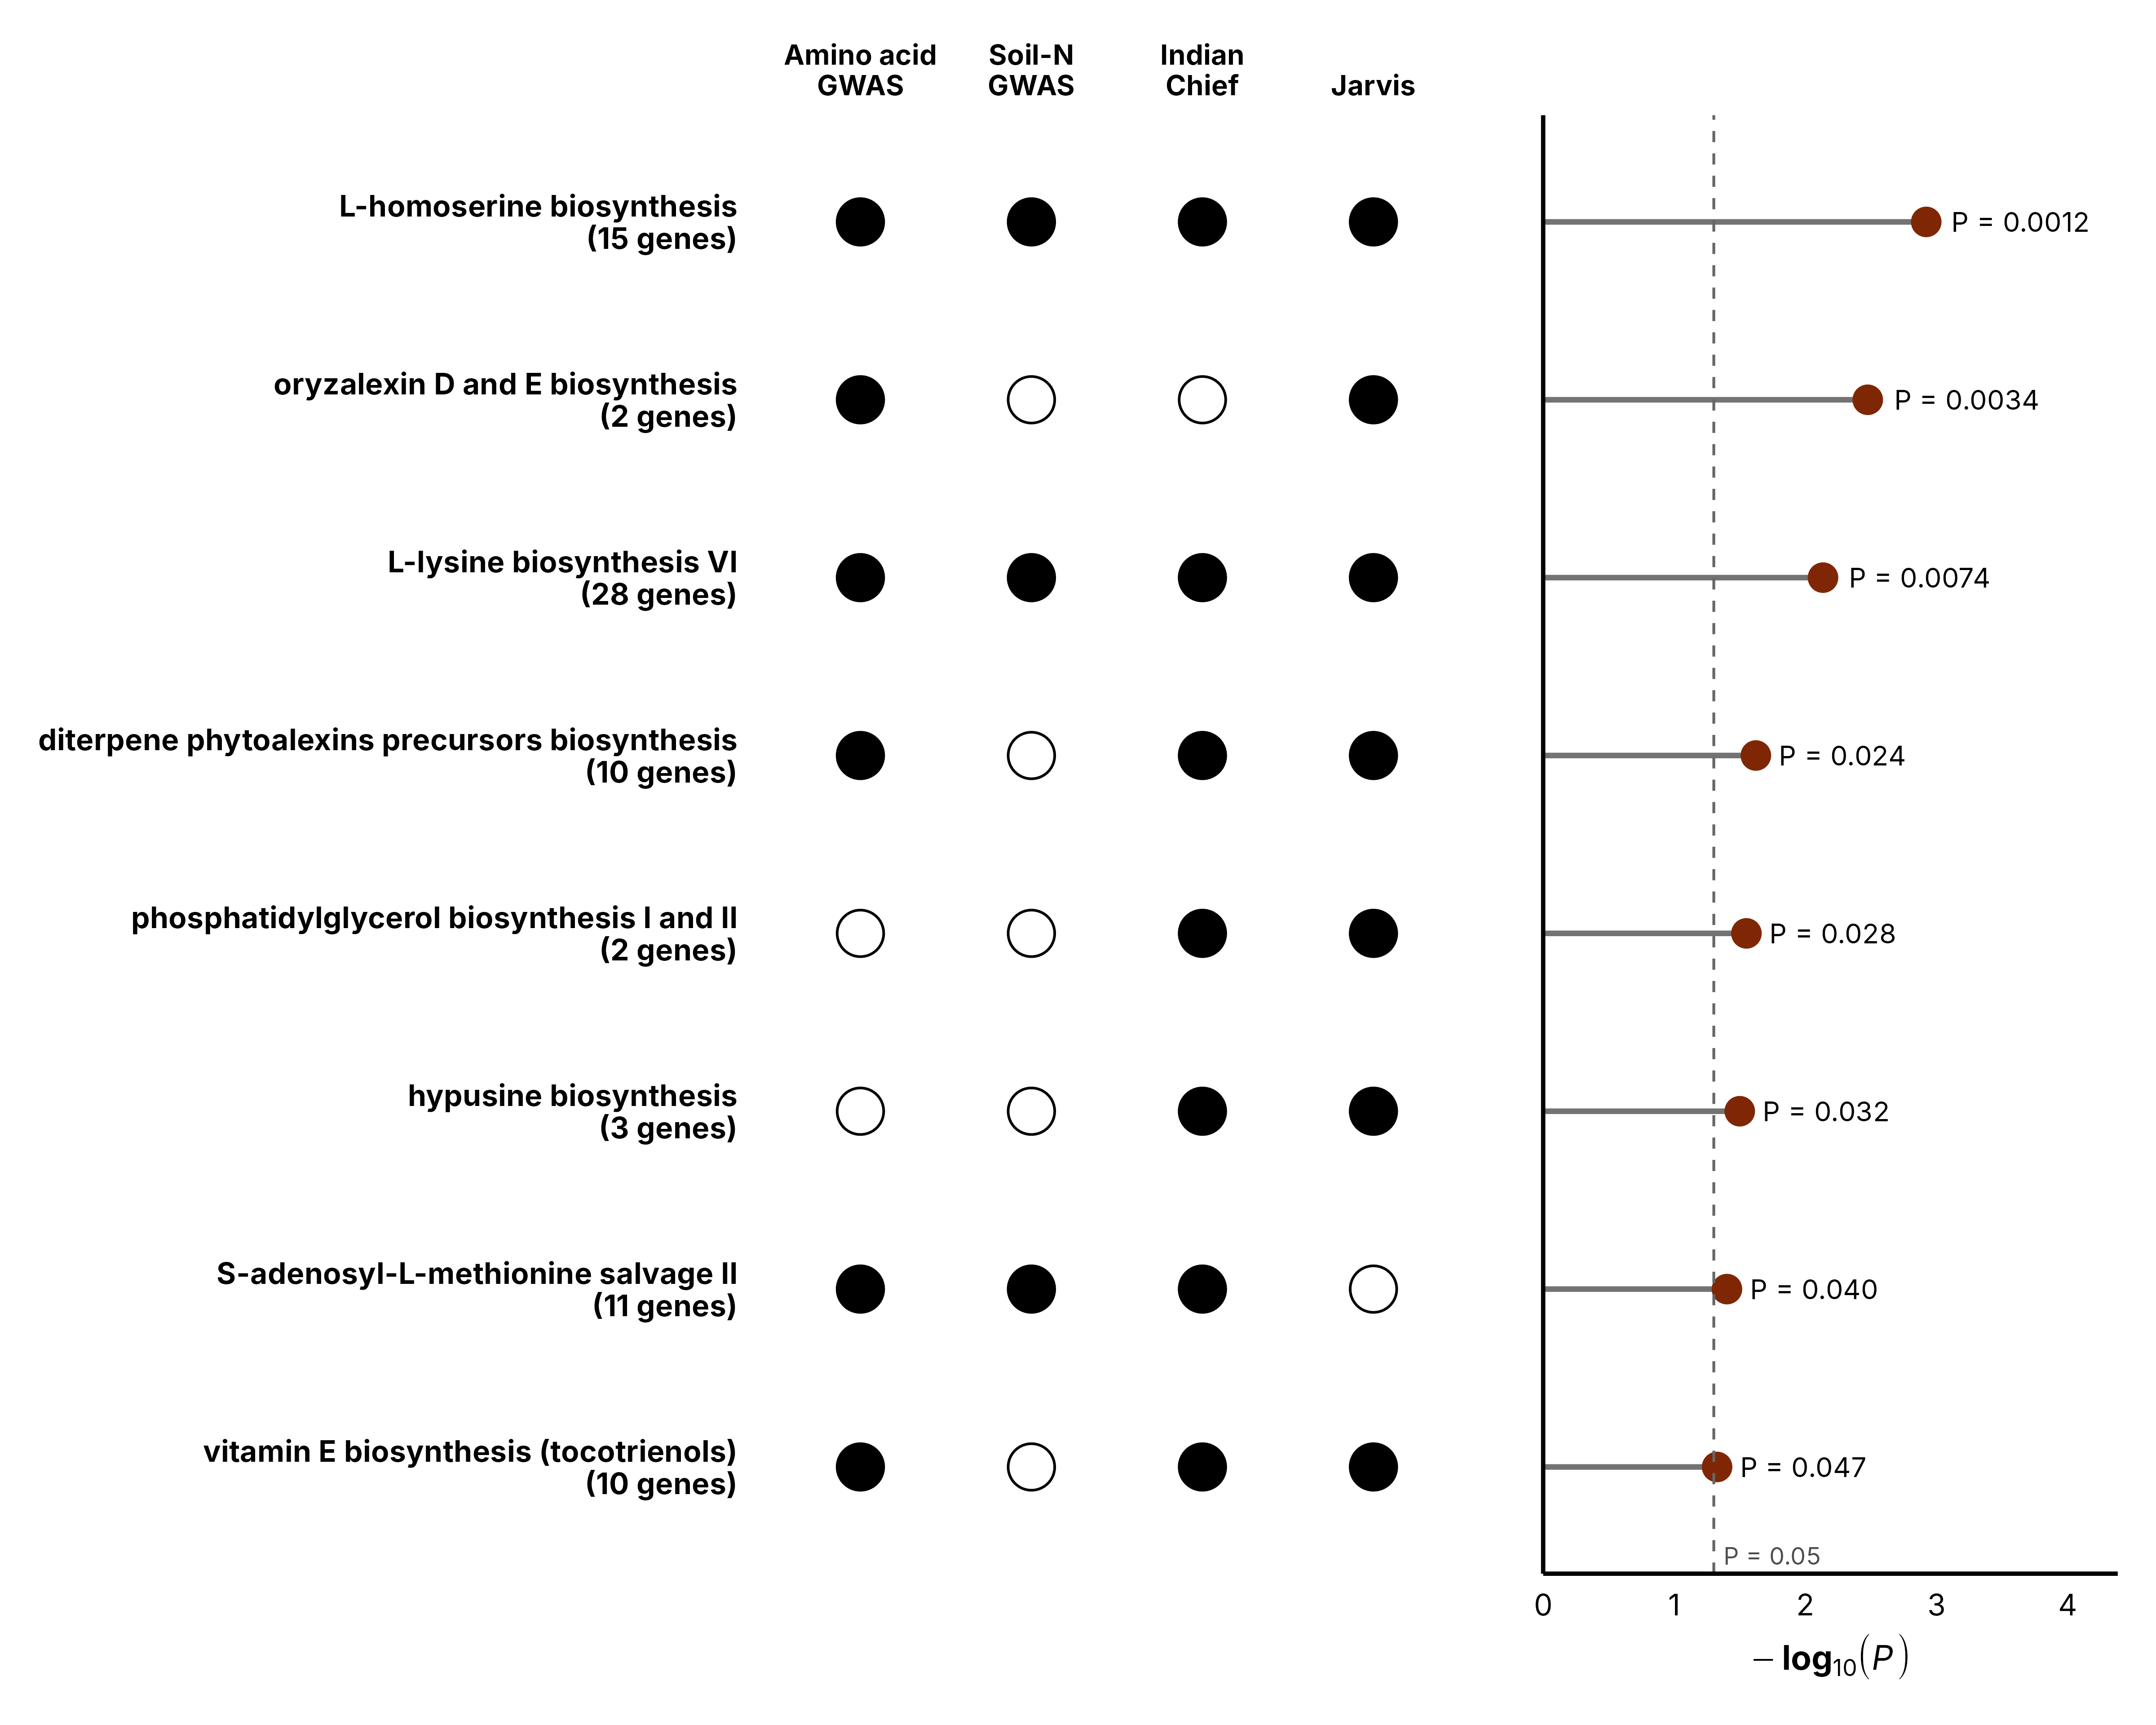
\includegraphics[width=\textwidth]{final/main_figs/Fig_pathway_recurrence.png}
    \caption{\textbf{The L-homoserine biosynthesis pathway recurs across all four analyses.} All CornCyc pathways with uncorrected permutation $P < 0.05$ for recurrence across the amino acid GWAS, soil-N GWAS and the Indian Chief and Jarvis $F_{ST}$ scans. Left, filled circles mark analyses with at least one candidate gene in the pathway; numbers in brackets give the number of maize genes in the pathway. Right, pathway-specific permutation $P$ (uncorrected) for the observed number of analyses hitting the pathway, from 20,000 genome-wide shifts of each analysis's candidate intervals; dashed line, $P = 0.05$. Phosphatidylglycerol biosynthesis I and II have identical gene sets and are shown once. L-lysine biosynthesis VI is hit through the same genes as L-homoserine biosynthesis. No pathway remained significant after correction for all 468 pathways.}
  \label{fig:pathway_recurrence}
\end{figure*}

\section{Discussion}\label{sec12}

The results support a model in which maize grain N variation arises through multiple genetic pathways that implicate related biological functions. Across soil-N environmental GWAS, grain amino acid GWAS, Indian Chief and Jarvis population-genomic scans, and exploratory B64 $\times$ CML14 biparental mapping, most candidate genes were specific to individual datasets, yet their annotations consistently involved connected N-remobilization and amino acid metabolism processes. We therefore interpret the study as consistent with shared functional themes rather than single-locus control. Candidate genes supporting this view are listed in Supplementary Table S21, and the conceptual model is shown in Fig.~\ref{fig:fig7_integrative_synthesis}. The following sections examine the main recurring functional modules and their implications for grain amino acid composition and N allocation.



% =========================
% FIGURE 7
% =========================
\begin{figure*}[!t]
    \centering
    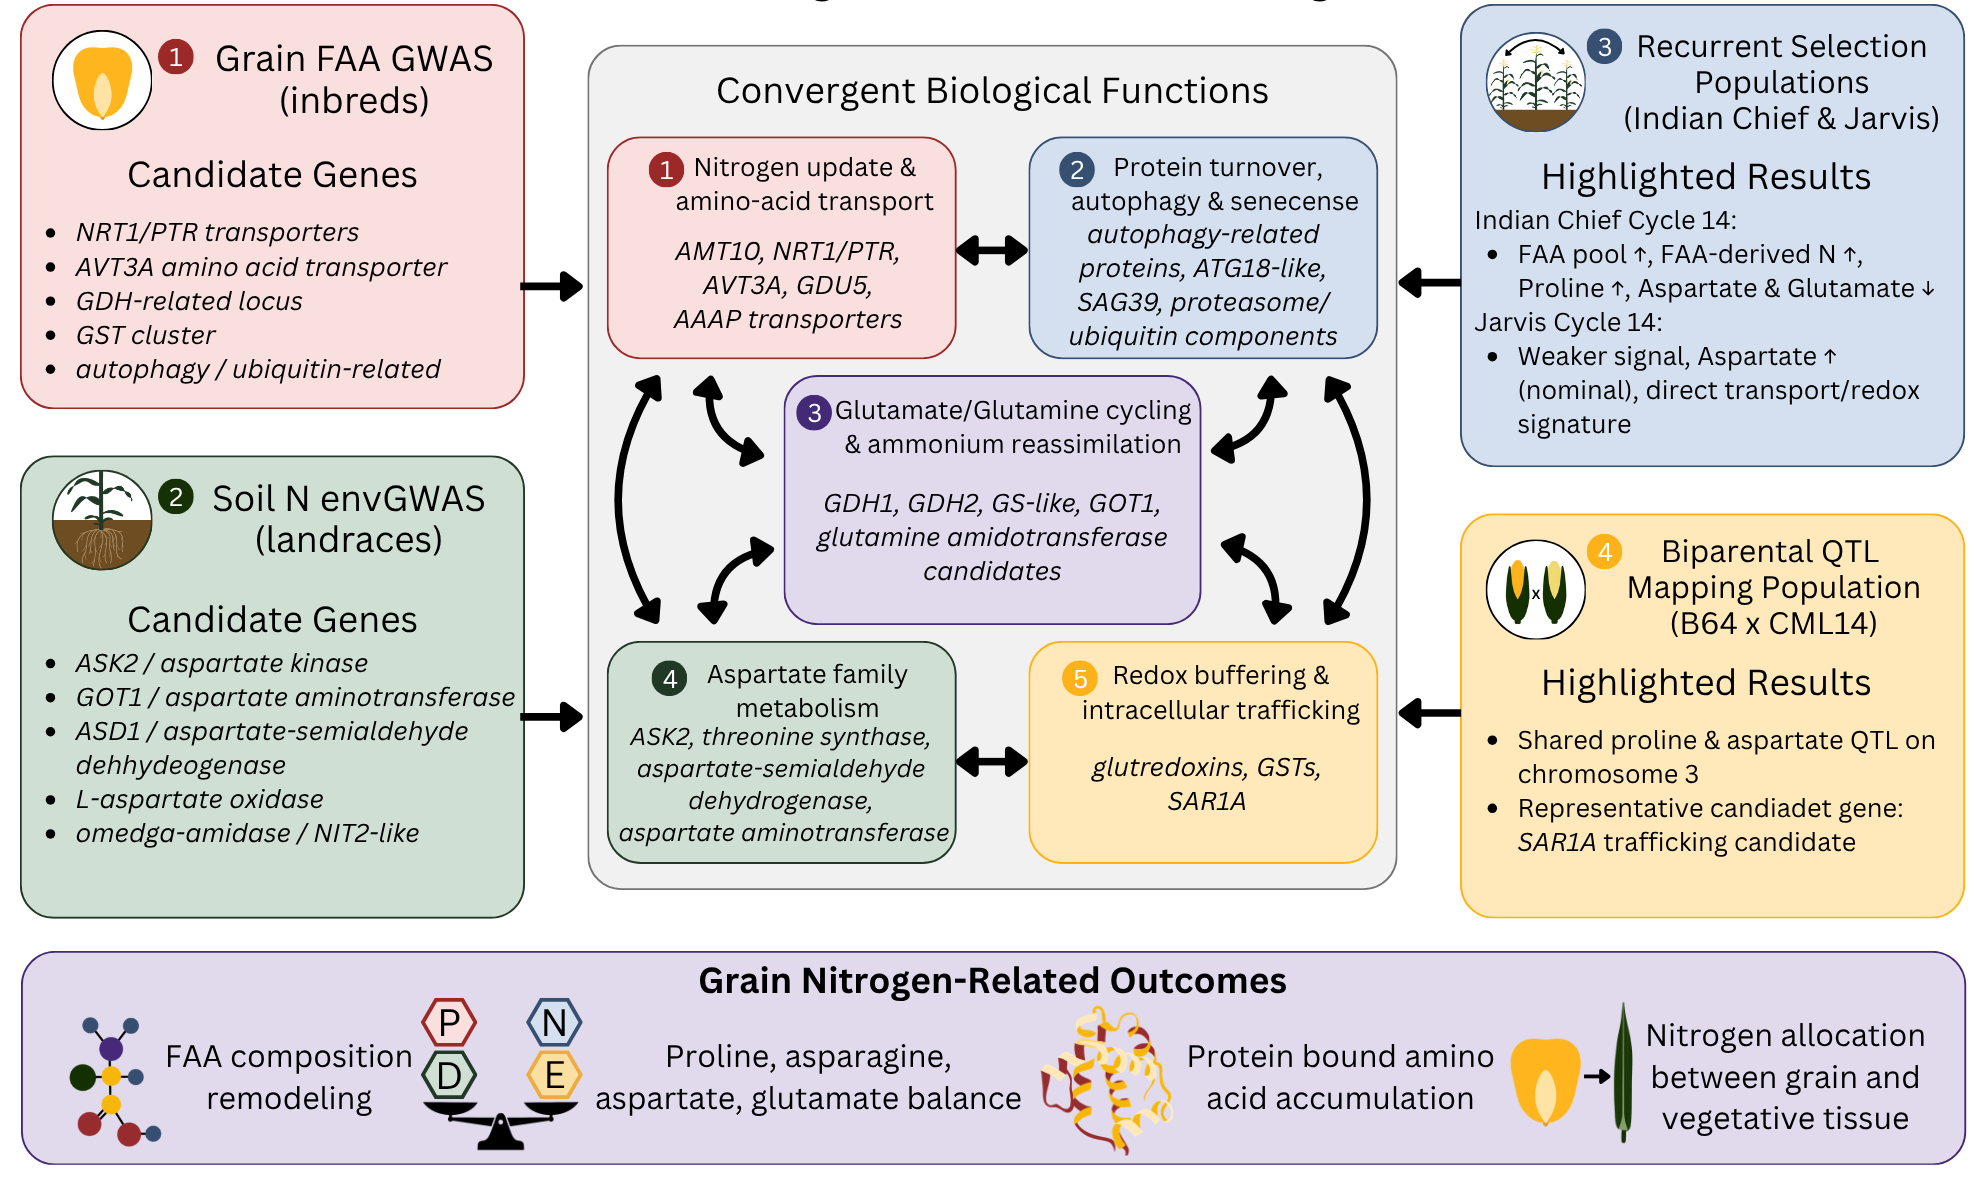
\includegraphics[width=\textwidth]{Figs/main/Fig7.png}
    \caption{\textbf{Integrative synthesis of genetic signals underlying maize grain nitrogen remodeling.}
    Candidate genes identified across grain free-amino acid GWAS, soil-N environmental GWAS, Indian Chief and Jarvis recurrent-selection population scans, and B64 $\times$ CML14 biparental QTL mapping were grouped by broad biological function.
    The figure summarizes shared pathway themes across candidate sets rather than repeated recovery of the same locus.
    Across datasets, candidate genes repeatedly implicated N uptake and amino acid transport, protein turnover, autophagy and senescence, Glu/Gln cycling and ammonium reassimilation, Asp-family metabolism, redox buffering, and intracellular trafficking.
    These functional modules provide mechanistic links to grain N-related outcomes, including free amino acid composition remodeling, Pro/Asn/Asp/Glu balance, protein-bound amino acid accumulation, and N allocation between vegetative tissues and grain.
    Candidate-gene details and dataset-level support are provided in Supplementary Table S21.}
    \label{fig:fig7_integrative_synthesis}
\end{figure*}


\subsection{Loci shared by many amino acid traits point to protein turnover and membrane protein biogenesis rather than specific biosynthetic steps}

Few GWAS loci were shared across many amino acid phenotypes, and shared loci were not near amino acid biosynthesis genes. Phenotype counts also overstate independent signals because composites and ratios reuse amino acids. The most interpretable case is the chromosome 4 locus at 174.57~Mb, associated with eight phenotypes (including alanine, valine, lysine, phenylalanine and threonine) spanning four biosynthetic families, and adjacent to \textit{Zm00001eb190800}, encoding a peptidase A1 (pepsin-like aspartic protease) (Fig.~\ref{fig:amino_locus_manhattan}). Aspartic proteases drive bulk protein turnover. In senescing tobacco, chloroplast CND41 degrades Rubisco, and reduced CND41 increases Rubisco retention under N limitation \citep{Kato2004CND41}. Because Rubisco breakdown is a major source of remobilized amino acids \citep{Feller2008Rubiscolytics}, and other A1 proteases function in development and stress \citep{Soares2019AtypicalAP}, a variant affecting multiple, unrelated amino acid pathways is more plausibly explained by altered protein degradation than by changes in a single biosynthetic enzyme, making \textit{Zm00001eb190800} a strong candidate.

The chromosome 9 locus implicates the endomembrane system. A $\sim$13~kb haplotype associated with seven phenotypes (including total free amino acids) spans \textit{Zm00001eb394360} to the 5$'$ end of \textit{Zm00001eb394380} and includes a significant SNP in \textit{Zm00001eb394380}. \textit{Zm00001eb394360} encodes ER membrane protein complex subunit 4, which inserts transmembrane proteins into the ER \citep{Guna2018EMC}, and \textit{Zm00001eb394380} encodes rhomboid-like protein 19, an intramembrane serine protease annotated to Golgi-to-ER retrograde transport. Although rhomboid functions in plants are poorly understood \citep{KnopfAdam2012Rhomboid}, both genes act in the ER--Golgi system that processes transporters and secreted proteins involved in amino acid and N movement \citep{Brandizzi2018ERGolgi}, so either could affect the overall free amino acid pool. Because the associations do not clearly separate these genes from nearby genes (including a DUF2404 membrane protein at the chromosome 4 locus), both loci should be treated as positional candidates, and kernel expression and mutant analyses are the most direct tests. Two additional loci associated with nine phenotypes are either $>$100~kb from any gene (chromosome 4, 212.55~Mb) or near a K homology domain RNA-binding protein of unknown function (\textit{Zm00001eb306240}, chromosome 7, 40.80~Mb) and are not discussed further. Candidate annotations, trait associations, and model-specific GWAS results are available at \url{https://j83gk2-nirwan-tandukar.shinyapps.io/amino_gwas_app/}.


\subsection{The aspartate-to-homoserine pathway links soil-N adaptation, recurrent selection, and grain amino acid variation}

Aspartate is a proteinogenic amino acid and N-bearing metabolic hub. Its carbon skeleton produces asparagine and the aspartate-family amino acids (lysine, threonine, methionine, isoleucine), and its amino group links to the glutamate pool via transamination \citep{Han2021Aspartate,Wang2018AspSeeds,Viola2001AspartatePathway}. Although the three populations shared no loci, all four analyses converged on this pathway. L-homoserine biosynthesis was the only CornCyc pathway with a candidate gene in every analysis and the least likely of 468 pathways to recur by chance ($P = 0.0012$, Fig.~\ref{fig:pathway_recurrence}). Each analysis implicated a different step: Jarvis top-5\% $F_{ST}$ regions included aspartate kinase (\textit{Zm00001eb094670}), the first committed step \citep{Viola2001AspartatePathway}; maize \textit{ask2} expression has been linked to methionine accumulation in developing kernels \citep{Duo2026Ask2}. The soil-N GWAS identified another aspartate kinase isozyme (\textit{Zm00001eb220040}) via its strongest SNP, significant in all three models. Indian Chief contributed aspartate-semialdehyde dehydrogenase (\textit{Zm00001eb214360}), and the amino acid GWAS implicated homoserine dehydrogenase (\textit{Zm00001eb405410}), the threonine/methionine branch point, through an intragenic SNP associated with the Asn fraction of the aspartate-family pool ($P = 3.0 \times 10^{-9}$). Downstream, Indian Chief regions included threonine synthase (\textit{Zm00001eb294790}) and methionine synthase (\textit{Zm00001eb052750}); the latter was also within 25~kb of a soil-N SNP, and \textit{S}-adenosyl-L-methionine salvage recurred in three analyses ($P = 0.040$). This recurrence was not significant after pathway-wide correction, and drift alone could generate the $F_{ST}$ candidate regions given $N_e \approx 25$--30 (Supplementary Fig.~\ref{fig:supp_ne_drift}); thus these genes are candidates, not confirmed selection targets.

Free amino acid profiles shifted differently between recurrent-selection populations (Fig.~\ref{fig:ic_j_faa}). In Indian Chief, total free amino acids and the proline fraction increased, while Asp and Glu fractions decreased; protein-bound amino acids did not change. In Jarvis, the Asp fraction increased only before multiple-testing correction. This matches the original experiment: Jarvis increased grain N mainly via higher grain weight and post-anthesis N uptake, whereas Indian Chief did not \citep{Moll1994}. Since grain N is largely protein-bound, Indian Chief likely remodeled the soluble pool from free Asp/Glu toward proline rather than increasing total grain N.

The amino acid GWAS identified lysine- and asparagine-branch candidates. On the lysine branch, 4-hydroxy-tetrahydrodipicolinate synthase (\textit{Zm00001eb389290}) and reductase (\textit{Zm00001eb176170}) were within 25~kb of SNPs for Asn ratios, and diaminopimelate decarboxylase (\textit{Zm00001eb406820}) carried a SNP for the Gln/Glu ratio ($P = 1.1 \times 10^{-9}$). On the asparagine branch, two asparagine synthetase domain genes (\textit{Zm00001eb036060}, \textit{Zm00001eb036070}) were near a SNP for the Asn/Glu ratio, and the transporter AVT6C (\textit{Zm00001eb368680}) was associated with free asparagine ($P = 1.3 \times 10^{-8}$) and the aspartate-family composite ($P = 2.5 \times 10^{-11}$) in both BLINK and FarmCPU, implicating transport or vacuolar storage as well as synthesis. Because soil N covaries with other landrace environmental features, soil-N candidates likely reflect adaptation via aspartate metabolism rather than grain composition per se. These genes are testable, for example by comparing aspartate-family amino acids among lines with alternative alleles at \textit{Zm00001eb405410}, \textit{Zm00001eb368680}, \textit{Zm00001eb094670}, and \textit{Zm00001eb214360}. Aspartate also links to the Glu/Gln pool via candidates such as an aspartate aminotransferase (Jarvis), an omega-amidase (soil-N GWAS), and the asparagine synthetases (which use glutamine-derived amide N), although no single Glu/Gln pathway recurred across analyses. We consider these links next.

\subsection{Candidate genes at the aspartate--glutamate junction link amino acid N with C--N recycling}

Aspartate and glutamate exchange amino groups with the TCA intermediates oxaloacetate and 2-oxoglutarate; thus, their intersection helps balance amino acid N with carbon skeletons \citep{Han2021Aspartate}. No glutamate/glutamine pathway recurred across analyses as L-homoserine biosynthesis did, so we discuss candidate junction genes individually. In Jarvis, top-5\% $F_{ST}$ regions included \textit{Zm00001eb152450} (GOT1), an aspartate aminotransferase that reversibly interconverts aspartate + 2-oxoglutarate with oxaloacetate + glutamate, potentially shifting Asp/Glu pool sizes \citep{Han2021Aspartate,Zhou2009AspAT}. GOT1 was recently identified as \textit{THP3}; teosinte alleles enhance N assimilation and seed protein in maize \citep{Huang2026THP3}. In the soil-N GWAS, a SNP in \textit{Zm00001eb005710} (NIT2; omega-amidase) was significant in two models. Omega-amidase completes asparagine/glutamine transaminase pathways by hydrolyzing 2-oxosuccinamate to oxaloacetate and 2-oxoglutaramate to 2-oxoglutarate, releasing ammonia \citep{Zhang2014OmegaAmidase} and returning amide N to the aspartate and glutamate carbon skeletons.

In Indian Chief, the top-5\% $F_{ST}$ regions included glutamate dehydrogenase (\textit{Zm00001eb060520}), an NADP-specific glutamate dehydrogenase family gene (\textit{Zm00001eb162300}), and a glutamine synthetase catalytic domain protein (\textit{Zm00001eb162900}). Plant glutamate dehydrogenase interconverts glutamate, 2-oxoglutarate, and ammonium; although not a primary ammonium assimilation route, GDH-deficient mutants show reduced glutamate catabolism and altered amino acid profiles under carbon limitation \citep{Miyashita2008GDH,Dellero2020AminoNUE}. Glutamine synthetase assimilates ammonium into glutamine, and cereal GS isoforms support N remobilization and glutamine supply to developing grain \citep{Wei2021WheatGS,Fujita2022RiceGS13}. Along with lower grain Glu and higher proline in Indian Chief Cycle~14, these candidates suggest altered glutamate turnover rather than increased primary N assimilation.

Grain amino acid GWAS highlighted GS/GOGAT-cycle genes that assimilate ammonium into glutamate, the amino-group donor for aspartate and asparagine. A GOGAT-like glutamine amidotransferase type 2 (\textit{Zm00001eb329710}) lay 1.0~kb from a SNP for the Asn/Glu ratio ($P = 6.1 \times 10^{-10}$); NADH-dependent glutamate synthase (\textit{Zm00001eb360480}) lay within 25~kb of a SNP for the lysine fraction of the aspartate-family pool ($P = 2.8 \times 10^{-11}$); and a glutamine synthetase domain gene (\textit{Zm00001eb059870}) lay within 25~kb of a SNP for the isoleucine fraction of the branched-chain pool. One gene overlapped selection scans and GWAS: \textit{Zm00001eb217220} (class-I glutamine amidotransferase domain) lay in an Indian Chief top-5\% $F_{ST}$ region and carried a SNP for free proline ($P = 2.2 \times 10^{-9}$), the amino acid whose fraction increased most after selection. Because glutamine amidotransferases act in many pathways, \textit{Zm00001eb217220} cannot be assigned to the Glu/Gln cycle without functional evidence, though rice \textit{FLOURY ENDOSPERM19} affects grain filling and C--N metabolism \citep{Lou2021FLO19}. Overall, both populations implicate genes near the aspartate/asparagine/glutamate/glutamine node linking N exchange with TCA-cycle carbon, but via different genes and without pathway-level support; thus they are candidates for follow-up, not evidence of a shared mechanism.

\subsection{Amino acid transport and protein turnover candidates}

Beyond aspartate and glutamate metabolism, the candidate sets contain genes for amino acid transport and protein turnover. These are individual candidates rather than recurring pathways, and they suggest processes worth testing rather than mechanisms.

Protein-turnover candidates were most relevant to Indian Chief, where Cycle~14 grain had higher free amino acids but unchanged protein-bound amino acids. Indian Chief candidate regions included \textit{Zm00001eb352300}, homologous to Arabidopsis \textit{ATG18a} (autophagosome formation during nutrient stress and senescence) \citep{Xiong2005ATG18a}, and \textit{Zm00001eb214780}, a senescence-specific cysteine protease related to \textit{SAG12} involved in N allocation during senescence and seed production \citep{James2018SAG12} and localized to senescence-associated vacuoles \citep{Otegui2005SAV}. The same window also contained \textit{Zm00001eb214890}, homologous to the Arabidopsis ammonium transporter \textit{AtAMT2} \citep{Neuhaeuser2009AtAMT2}. Increased protease activity in Cycle~14 could raise the free amino-acid pool via protein degradation, matching the Indian Chief phenotype, though drift could also explain these regions. In contrast, Jarvis candidate regions included amino acid transporters—an LHT-like transporter (\textit{Zm00001eb132750}) \citep{Fan2023LHT} and a PROT-like transporter (\textit{Zm00001eb159580}) \citep{Lehmann2011ProT}—plus NPL4-like protein~1 (\textit{Zm00001eb146560}), which functions in ubiquitin-dependent protein degradation.

The amino acid GWAS implicated transporter genes in specific traits. A SNP in NRT1/PTR family 4.6 \textit{Zm00001eb277160} was associated with the lysine fraction of the free pool in both BLINK and FarmCPU ($P = 2.5 \times 10^{-11}$). Three UmamiT (WAT1-related) genes were linked to aspartate- and glutamate-family traits: \textit{Zm00001eb379220} harbored a SNP for free glutamine ($P = 1.2 \times 10^{-11}$), \textit{Zm00001eb207630} to the aspartate fraction of the aspartate-family pool, and \textit{Zm00001eb352400} to the lysine fraction of the same pool. A chromosome 6 transporter cluster (\textit{Zm00001eb261470}--\textit{Zm00001eb261490}) was associated with the Gln/Glu ratio, and a cationic amino acid transporter (\textit{Zm00001eb050630}) contained a SNP for the branched-chain composite. Two loci suggested vacuolar storage: \textit{AVT3A}-like \textit{Zm00001eb429100} was 17~kb from a SNP for the isoleucine fraction of the LAV composite ($P = 1.1 \times 10^{-7}$); Arabidopsis AVT3 proteins export amino acids from the vacuole \citep{Fujiki2017AtAVT3}; and AVT6C-annotated \textit{Zm00001eb368680} was associated with free asparagine. Overall, variation in amino acid transport and storage, not just biosynthesis, appears to shape the grain free amino acid pool.


\section{Conclusion}\label{sec13}
%Sarah is still working on this 

By integrating soil-N environmental GWAS, grain amino acid GWAS, recurrent-selection population genomics, and biparental QTL mapping, we show that maize grain nitrogen composition is associated with variation across multiple, partially overlapping biological pathways rather than control by a single conserved locus or a small number of major-effect loci.

\quad Across independent datasets, we identify candidate genes falling into four broad functional categories: (1) aspartate-family metabolism, which governs allocation of nitrogen into essential amino acid biosynthetic pathways; (2) Glu/Gln-centered C--N cycling, linking nitrogen assimilation and reassimilation with central carbon metabolism; (3) amino acid transport and intracellular partitioning; and (4) protein turnover and recycling through autophagy- and ubiquitin-mediated pathways. Support for the relevance of these processes comes from GWAS signals for amino acid transporters, dehydrogenases, and Asp-family enzymes; soil-N associations implicating asparagine, glutamine, and aspartate-related metabolism in environmental adaptation; selection-driven FAA remodeling and population-specific differentiation in Indian Chief and Jarvis; and a shared Pro/Asp QTL implicating ER-to-Golgi trafficking.

\quad Importantly, the recurrent-selection populations demonstrate that substantial shifts in grain amino acid composition can arise through distributed allele-frequency changes across these pathways. Indian Chief exhibited expansion of the FAA pool, increased FAA-derived N, and strong proline enrichment with reduced Asp and Glu fractions, while PBAA-derived and total amino acid-derived N pools did not change significantly. This indicates that the strongest Indian Chief response was concentrated in the soluble amino acid pool rather than reflecting a uniform increase across all grain amino acid pools. In contrast, Jarvis showed weaker phenotypic shifts but contained candidate loci directly linked to aspartate-family biosynthesis. These contrasting outcomes suggest that similar selection pressures may reshape grain nitrogen allocation through distinct genetic routes within a partly shared metabolic network.

Since the Indian Chief and Jarvis populations were advanced via reciprocal recurrent selection based on hybrid performance rather than fully isolated selection, they should not be viewed as completely independent. Although they did not directly mix, selection decisions relied on their cross performance, creating a shared breeding context. Moreover, with 14 selection cycles, some allele-frequency changes and outliers may reflect drift or other stochastic effects rather than selection alone. We therefore treat the Indian Chief–Jarvis contrasts as complementary evidence for selection-associated remodeling of grain nitrogen traits, while acknowledging that drift and the reciprocal selection design may also have contributed to the observed genomic differentiation.

\quad Together, these results support a model in which maize grain nitrogen variation is governed by distributed modulation of N flux, protein turnover, amino acid transport, and intracellular trafficking during kernel development. In this framework, FAA and PBAA pools are not passive storage forms but dynamic products of coordinated metabolic and cellular processes. Perturbation of aspartate-family enzymes should shift the balance of nitrogen among downstream amino acid pools; manipulation of glutamate dehydrogenase, glutamine synthetase, or aminotransferases should alter C--N recycling and FAA accumulation; and disruption of protein trafficking or autophagy pathways should affect the partitioning between soluble and storage-protein-bound amino acids. Future functional studies targeting these processes will be critical to resolving causal mechanisms.

\quad From an applied perspective, our findings suggest that optimizing maize grain N allocation while maintaining agronomic performance will likely require coordinated modification of multiple pathways rather than targeting a single locus. Candidate targets include regulators of Asp-family flux, Glu/Gln cycling enzymes, amino acid transporters, and components of protein turnover and trafficking systems. By identifying recurrent functional themes across candidate sets, this study provides a framework for breeding and engineering strategies aimed at improving nitrogen use efficiency and reducing fertilizer-associated nitrogen losses in maize production systems \citep{OjedaRivera2025NitrogenEfficientMaize}.



\section{Methods}\label{methods}

\subsection{Germplasm used}
\subsubsection{Maize Landraces}
The maize landraces discussed by Romero Navarro et al. (\cite{RomeroNavarro2017Landraces}) come from the CIMMYT International Germplasm Bank collection, which contains over 24,000 accessions of traditional maize varieties primarily from North, Central, and South America. They characterized a core collection of 3,511 genotypes based on availability of accurate geographic coordinates and complete environmental data for their collection locations. These landraces are genotyped using genotyping-by-sequencing (GBS) at about 2X coverage, with SNP calling and imputation for analysis. The population represents a geographically and genetically diverse panel that serves as an important resource for studying environmental adaptation, such as soil N availability.


\subsubsection{Indian Chief and Jarvis (IC and J)  }
We worked with two open-pollinated maize populations Indian Chief (IC) and Jarvis (J) from Moll \textit{et al.}~\citep{Moll1994} that underwent reciprocal recurrent selection for 14 generations for grain yield. Beginning from base populations (G$_0$), each cycle involved intercrossing the best families selected on hybrid (IC$\times$J) performance and advancing through a selfed recombination nursery.

\subsubsection{Indian Chief and Jarvis recurrent-selection populations}

We used two open-pollinated maize populations, Indian Chief (IC) and Jarvis Golden Prolific (J), from the recurrent-selection experiment described by \citet{Moll1994}. These populations underwent 14 cycles of reciprocal recurrent selection for grain yield. In this scheme, parents within each population were selected based on the performance of their hybrid progeny in the IC~$\times$~J population, and selfed progeny from the selected parents were intermated to generate the next selection cycle. For the present study, individuals from the base populations, Cycle~0 (C0), and the selected populations, Cycle~14 (C14), were analyzed for both Indian Chief and Jarvis. Because selection in each population was based on hybrid performance with the other population, the evolutionary trajectories of Indian Chief and Jarvis are not fully independent: allele-frequency changes in one population over successive cycles were partly shaped by the genetic composition of the other. No gene flow occurred between the populations, but this correlated selection history should be considered when interpreting population-specific signals.

For amino acid profiling, Indian Chief and Jarvis Cycle 0 and Cycle 14 plants were grown in 2025 at the Central Crops Research Station (Clayton, NC) under standard field management using a randomized complete block design. The whole cob was collected and stored until analysis.

\subsubsection{The Goodman-Buckler Maize Association Panel}
%\rra{I know we are close the the 4th and patriotic spirits (https://www.youtube.com/watch?v=JYqfVE-fykk) are high but use celsius for temperature}
The Goodman-Buckler maize association panel (Flint-Garcia et al., 2005)  was grown at Genetics Farm near Columbia Missouri in 2017 and 2018 in two replicates each, in a randomized complete block design. Of the 282 lines in this panel, only 280 were grown successfully. 13 kernels of each line were planted in a 10 foot row and self-pollinated. At full physiological maturity, the pollinated ears were harvested, husk leaves were removed, and were subsequently dried at 40 degrees celcius and <20 relative humidity for 5 days to remove moisture from the grain. Ears from each line in each rep and year were shelled and bulked to form four representative composite grain samples for each of the 280 lines. For phenotypic evaluation, 25 random seeds were selected from each bulked sample to be ground and prepared for amino acid extraction and quantification

\subsubsection{Bi-parental Mapping Population}
The bi-parental QTL mapping population was developed by crossing the two inbred lines of the Goodman-Buckler Association Panel with the lowest and highest free Asn accumulation in the grain, B64 and CML14, respectively. F2:3 families were grown in two complete randomized blocks in 2024 at Genetics Farm near Columbia Missouri. For each plot, 13 kernels were planted in a 10-foot row and sib-pollinated to produce three ears. At full physiological maturity, the pollinated ears were harvested, husk leaves were removed, and ears were subsequently dried at 41 degrees Celsius and 20\% relative humidity for 5 days to remove moisture from the grain. From each ear, 10 representative kernels were sampled, then bulked, ground, and prepared for amino acid extraction and quantification.


\subsection{Phenotypic Evaluation}
\subsubsection{Grain/Stover Nitrogen}

Grain and stover N concentrations for all Indian Chief (IC) and Jarvis (J) lines were previously determined for the base generation (G$_0$) and the 14th cycle of selection (G$_{14}$) by Moll \textit{et al.}~\citep{Moll1994}. At a high fertilizer rate of $224~\mathrm{kg~N~ha^{-1}}$, J$_{14}$ produced heavier kernels and had higher grain N concentration than the original J$_0$ line. Post-anthesis N uptake from the soil supplied nearly all of this additional grain N, whereas the amount of N remobilized from stover to grain remained largely unchanged.

Indian Chief showed a contrasting response. In IC$_{14}$, vegetative biomass increased, but grain weight and grain N concentration remained similar to IC$_0$. The loss of N from stover after flowering was lower than in the base generation, indicating that more N was retained in stems and leaves and less was transferred to the grain. Thus, 14 cycles of selection increased grain N in Jarvis primarily through greater post-anthesis N uptake, whereas Indian Chief retained more N in vegetative tissue and showed little change in grain N concentration~\citep{Moll1994}.


\subsubsection{Soil nitrogen}
The environmental phenotype, soil total N, was derived from ISRIC global soil datasets \citep{Batjes2006ISRICWISE5ArcMin}. Values for the 0--5~cm and 5--15~cm layers were assigned to the collection coordinates of each landrace accession; 0--5~cm was used as the primary GWAS phenotype and 5--15~cm as a check. Because soil N is an environmental estimate rather than a plant measurement, GWAS results were interpreted as historical associations with soil N.


\subsubsection{Amino Acid Profiling}
% \rra{add these references to the bibliography}
PBAAs were extracted and quantified as described in \cite{Yobi2018PBAA}. This protocol utilizes microscale protein hydrolysis and absolute quantification using multiple reaction monitoring-based liquid chromatography–tandem mass spectrometry detection. During acid hydrolysis, Gln and Asn are converted into Glu and Asp, respectively. Therefore, we denote both Gln and Glu as Glx and Asn and Asp as Asx. During the extraction, Trp and Cys were fully destroyed, and Gly was poorly detected; therefore, these three amino acids were excluded from the dataset. In total, 15 PBAAs were analyzed to represent 17 PBAAs. FAAs were extracted and quantified as described in (Gu et al., 2007). Unlike the protocol above, all 20 proteinogenic amino acids were independently and successfully detected using UPLC-MS/MS.


\subsection{Sequencing and genotyping}

\subsubsection{Indian Chief and Jarvis}
% \rra{the sequencing sample sheet / variant-count table cited in this section as Supplementary Table S1 and S2 do not match with what's in the supplement where S1 is FAA phenotype values and S2 is amino acid abbreviations.}

Genome-wide coverage estimated with \texttt{Picard CollectWgsMetrics} and including zero-depth positions ranged from 0.28$\times$ to 0.38$\times$ across the four population--cycle groups. In contrast, sample-level mean depth calculated from the retained variant set averaged 0.73$\times$ across the 379 analyzed individuals (median 0.72$\times$, range 0.32--1.91$\times$). Each group initially included 96 individuals, for a total of 384 samples. These populations were generated after 14 cycles of reciprocal recurrent selection for increased grain yield \citep{Moll1994}. Paired-end Illumina libraries were constructed and sequenced as 2~$\times$~150~bp reads on a NovaSeq~6000 platform. Raw base-call files were demultiplexed with \texttt{fqtk} v0.3.1, yielding one 96-sample plate for each population--cycle group.

Adapter trimming and quality filtering used \texttt{fastp} v0.23.4, and read quality was assessed with \texttt{FastQC} v0.12.1. Trimmed reads were aligned to the B73 NAM reference genome RefGen\_v5 (GCF\_902167145.1) with \texttt{BWA-MEM} v0.7.18. Alignments were coordinate-sorted, duplicates were collapsed with \texttt{Picard MarkDuplicates} v3.1.1, and read groups were standardized with \texttt{Picard AddOrReplaceReadGroups}. Variant discovery followed the GATK Best Practices joint-genotyping workflow using \texttt{GATK} v4.5.0.0. Joint genotyping was performed per chromosome with \texttt{CombineGVCFs} and \texttt{GenotypeGVCFs}, generating 10 per-chromosome VCFs that were merged into a cohort VCF with 80,728,251 raw variant sites. Five low-quality samples (I14\_A07, I14\_B06, I14\_D05, I14\_F12, J14\_H11) were removed, leaving 379 genomes for population-genomic analysis. Genome-wide coverage was estimated with \texttt{Picard CollectWgsMetrics}. Genome-wide mean coverage (including zero-depth positions) was 0.28× for I01, 0.38× for I14, 0.32× for J01, and 0.37× for J14, consistent with low-pass skim sequencing (Supplementary Fig.~S1). SNPs and indels were filtered with GATK hard-filtering criteria, yielding 59,199,563 high-confidence variants, including 52,543,238 SNPs and 6,656,325 indels across the 10 maize chromosomes and scaffolds. The filtered SNP set was used for downstream population-genomic analyses.


\subsubsection{The Goodman-Buckler maize association panel}
% \rra{add citations to bibliography. This paragraph says candidate genes withi 25Kb / p<0.001 but the proxy-N below says 100Kb, and the results section say -log10(p)>=7. We have to make the window and threeshold consistent across GWASes or explain why we don't}

The Goodman-Buckler maize association panel had been previously genotyped with both the Illumina MaizeSNP50 BeadChip (\cite{FlintGarcia2005Goodman}) and with genotyping-by-sequencing (GBS) method as described in (Lipka et al., (2013). We filtered SNPs by minor allele frequency greater than 0.05 prior to analysis. We conducted amino acid GWAS using the HAPPI pipeline, which implements the GAPIT MLM, MLMM, FarmCPU, and BLINK models for univariate association mapping. Following the GWAS, we used fixed significance threshold of $-\log_{10}(p) \ge 7$ to correct the multiple hypothesis testing problem. Using the Maize AGP\_V5, we identified candidate genes within 25kb on either side of SNPs. 

\subsubsection{Bi-parental Mapping Population}
Leaf tissues were collected from F2 plants and lyophillized prior to DNA extraction and genotyping using the mid-density temperate corn panel by Agriplex Genomics (Cleveland, OH).

\subsection{Population-genomic analyses}

\subsubsection{Genotype-likelihood framework}

Population-genomic statistics were estimated using ANGSD v0.941 \citep{Korneliussen2014ANGSD}, which is appropriate for low-coverage sequencing because it uses genotype likelihoods rather than hard genotype calls. Analyses were performed separately for Indian Chief Cycle~0 (IC\_C0), Indian Chief Cycle~14 (IC\_C14), Jarvis Cycle~0 (J\_C0), and Jarvis Cycle~14 (J\_C14). The same read- and base-level filtering parameters were applied across all population--cycle groups to ensure comparable estimates among contrasts.

For each population--cycle group, site allele-frequency likelihoods were estimated with ANGSD and stored as SAF files. For pairwise analyses, joint two-dimensional site-frequency spectra were estimated from the corresponding SAF files using \texttt{winsfs}, a window-EM SFS estimator, to improve computational efficiency. These joint spectra were then used as priors for downstream $F_{ST}$ estimation.

\subsubsection{Differentiation between cycles}

Allele-frequency change between Cycle~0 and Cycle~14 was measured separately in Indian Chief (IC\_C0 versus IC\_C14) and Jarvis (J\_C0 versus J\_C14) with $F_{ST}$. For each contrast, a joint two-dimensional site-frequency spectrum was estimated from the SAF files with \texttt{winsfs} \citep{Rasmussen2022winsfs} and used as the prior for \texttt{realSFS fst index}. Per-site $F_{ST}$, the ratio of the per-site numerator and denominator reported by \texttt{realSFS fst print}, was summarized along each chromosome with the GenWin smoothing-spline method (\texttt{splineAnalyze}; smoothness 500~kb, method~4) \citep{Beissinger2015GenWin}, which places window boundaries at inflection points of a spline fitted to $F_{ST}$ rather than at fixed intervals. This produced 2,162 windows in Indian Chief and 2,151 in Jarvis (median length 500~kb), each summarized by the mean per-site $F_{ST}$. Windows at or above the 95th percentile of the window $F_{ST}$ distribution of each population were retained as candidate regions. These are empirical outliers rather than significance thresholds: at the effective population size of these populations, drift moves linked regions together, and no neutral distribution was derived for individual windows.

To compare candidate regions between populations, whose window boundaries differ, the genome was divided at every window boundary of either population, and each resulting segment was assigned the $F_{ST}$ of the Indian Chief window and of the Jarvis window that contained it. Overlap was measured as the number of base pairs (in 10-kb bins) in the top 5\% in both populations and compared with 10,000 circular shifts of the Jarvis candidate track along the concatenated chromosomes, which preserve the size and clustering of candidate windows. Concordance of window $F_{ST}$ between populations was summarized with Spearman's correlation across segments.

\subsubsection{Effective population size}

In the reciprocal recurrent selection program, each cycle was formed by intermating, within each population, the self-pollinated progenies of the 20 plants whose half-sib testcross progenies with the other population had the highest grain yield \citep{MollStuber1971}. Testcross progenies were used only for evaluation, so no alleles were exchanged between populations, and each cycle involved a single sampling of parents from the previous cycle. Neutral allele-frequency change under this scheme is therefore expected to follow a Wright--Fisher process with one generation per cycle and an effective population size ($N_e$) of at most 20, the value reached when all selected parents contribute equally.

To compare the observed differentiation with this expectation, we estimated $N_e$ for each population from the allele-frequency change between Cycle~0 and Cycle~14. Per-site allele frequencies for each population--cycle group were taken from ANGSD \citep{Korneliussen2014ANGSD}, retaining sites with data for at least 30 individuals in both cycles and with the same major and minor alleles in both cycles. Sites were grouped into non-overlapping 250-kb windows (at most 400 randomly chosen sites per window; 8,524 windows in Indian Chief and 8,527 in Jarvis), Hudson's $F_{ST}$ \citep{Bhatia2013Fst} between Cycle~0 and Cycle~14 was computed per window as a ratio of sums, and the genome-wide mean was taken across windows. We then simulated neutral Wright--Fisher drift for 14 generations, starting each site at its observed Cycle~0 frequency, for $N_e$ = 20, 30, 50, 75, 100, 150, 250, and 500. At both time points, simulated frequencies were resampled using the number of individuals with data at each site, and $F_{ST}$ was computed with the same estimator as for the observed data. $N_e$ was taken as the value at which the simulated genome-wide mean $F_{ST}$ matched the observed value, interpolating linearly between grid points. Because the simulation does not model linkage, it was used only to estimate genome-wide $N_e$ and not to test individual windows.

\subsubsection{Population structure, principal component analysis, and between-population differentiation}

Because sequencing depth differed between cycles, population structure was inferred from genotype likelihoods rather than hard-called genotypes. Phred-scaled genotype likelihoods (GATK \texttt{PL}) for all 379 individuals were taken from the filtered VCF and converted to Beagle genotype-likelihood format; individuals without reads at a site were given uninformative likelihoods. Sites were retained if at least 50\% of individuals had reads and the likelihood-weighted minor allele frequency was at least 0.05, and were thinned to one site per 10~kb to reduce linkage, leaving 82,061 sites. Admixture proportions were estimated with NGSadmix \citep{Skotte2013NGSadmix} for $K = 2$--5 with three independent seeds per $K$; $K$ was chosen as the largest value at which runs converged to the same likelihood and solution. Principal component analysis was performed on the genotype-likelihood covariance matrix estimated with PCAngsd \citep{Meisner2018PCAngsd} from the same sites. Differentiation between Indian Chief and Jarvis was estimated separately at Cycle~0 and Cycle~14 from joint two-dimensional site-frequency spectra estimated with \texttt{winsfs} \citep{Rasmussen2022winsfs} from the per-group ANGSD SAF files. Hudson's $F_{ST}$ \citep{Bhatia2013Fst} was computed from each spectrum as a ratio of averages over all sites, per chromosome and genome-wide.

\subsubsection{Candidate window annotation}
% \rra{remember to add B73 reference version here}

Top-5\% $F_{ST}$ windows were intersected with the maize B73 reference genome annotation RefGen\_v5 (AGPv5), and genes overlapping a candidate window were retained as candidate genes. Candidate genes were annotated with PANTHER family, protein class, and Gene Ontology terms (Supplementary Tables~S19--S20).

\subsubsection{Genome-wide association Studies}

\paragraph{Environment GWAS}

% \rra{this section requires much mor detail an information. See comments in the results about the nitrogen phenotype used. "Approximately 495,755 SNPs for maize landraces" this sentence is missing a verb. Add more information about the SNP source and filtering etc from Romero-Navarro etc. What is the significance threshold and what correction did you use Bonferroni, FDR?}

Genome-wide association analysis for soil N was performed in the maize landrace panel \citep{RomeroNavarro2017Landraces} using the 3,107 accessions with both genotype and soil N data and 495,755 SNPs aligned to Zm-B73-REFERENCE-NAM-5.0. Associations were tested with MLM, BLINK and FarmCPU \citep{Slaten2020HAPPI}, with three genotype principal components as covariates (Supplementary Fig.~\ref{fig:supp_pca_scree}). For each model, Benjamini--Hochberg FDR was computed over the full scan and SNPs with FDR $\leq 0.05$ were declared significant. Candidate genes were B73 RefGen\_v5 genes within 25~kb of a significant SNP. Functional interpretation used maize gene annotations, MaizeGDB, Phytozome, and Arabidopsis homology resources.

To test whether soil-N associations reflected geography or climate, we ran the same pipeline on latitude, longitude, elevation, soil pH, CEC and aridity (Ref). The overlap between the significant SNP sets of each pair of variables was compared with its chance expectation, $n_1 n_2 / M$ ($M = 495{,}755$), using a one-sided hypergeometric test. In a second, model-free test, we computed the Pearson correlation between allele dosage (0, 1, 2; missing genotypes set to the SNP mean) and each site variable across the 3,107 accessions for every SNP, and expressed each SNP's $|r|$ as a genome-wide rank. A soil-N SNP was called linked to the environment if it ranked in the top 1\% for any non-N variable, not linked if it ranked in the top 5\% for soil N and not in the top 1\% for any other variable, and inconclusive if it ranked outside the top 5\% for soil N. The share of soil-N SNPs in the top 1\% for at least one geographic or environmental variable was compared, by binomial test, with the whole genome and with SNPs in the top 1\% for correlation with soil N.

\paragraph{Metabolite GWAS}

% \rra{several missing pieces here. Make sure numbers match results. Here you say 110 FAA + 77 PBAA but in results you mention 78 amino acid derived results}
Metabolite GWAS was conducted in the Goodman--Buckler Association Panel \citep{FlintGarcia2005Goodman} using 4,177,796 SNPs from the maize HapMap 3.2.1 genotypes of the 282-line panel, which are positioned on the B73 AGPv4 assembly. The dataset included 78 amino acid-related phenotypes: absolute and relative free amino acid traits, amino acid family composites, biochemical ratios, and the proxy traits \textit{Total\_N} and \textit{Total\_PBAA}. For each phenotype, best linear unbiased predictions (BLUPs) were estimated before association analysis. GWAS used the HAPPI pipeline, which integrates phenotype preprocessing and association mapping and implements the GAPIT MLM, MLMM, BLINK, and FarmCPU models \citep{Slaten2020HAPPI}. Significance was declared at a 5\% Benjamini--Hochberg FDR, applied separately to each phenotype and model; MLMM gave no significant SNPs, so results come from MLM, BLINK and FarmCPU. Because the genotypes are on AGPv4, SNP positions were lifted to Zm-B73-REFERENCE-NAM-5.0 with the B73 RefGen\_v4-to-NAM-5.0 chain file, using same-chromosome forward-strand alignments and taking the highest-scoring alignment where several overlapped; 21 of the 2,461 significant SNPs fell in alignment gaps and were placed at the nearest aligned base. Candidate genes were B73 RefGen\_v5 genes within 25 kb upstream or downstream of each significant SNP, and significant SNPs within 25 kb of each other, across phenotypes, were merged into loci. A candidate gene was called trait-matched when its annotation (gene name and PANTHER family) placed it in the metabolism of the amino acid the phenotype reports on (the numerator amino acid, both amino acids of an amino acid ratio, or the members of a family composite) or of another amino acid in the same biosynthetic family, in amino acid, ammonium or nitrate transport, or in primary nitrogen assimilation (glutamine synthetase, glutamate synthase). This is a descriptive annotation, not an enrichment test.

To generate the \textit{Total\_N} proxy trait, amino acid measurements were converted to amino acid-derived nitrogen values by weighting each amino acid by its nitrogen content. For an amino acid $X$, the nitrogen mass fraction was calculated as

\[
\%N_X =
\left(
\frac{n_{N,X}\times M_N}{M_X}
\right)\times 100
\]

where $M_X$ is the molar mass of amino acid $X$, $M_N$ is the molar mass of nitrogen, and $n_{N,X}$ is the number of nitrogen atoms in amino acid $X$. amino acid-derived nitrogen for each amino acid was then calculated as

\[
N_X\;(\mu g/mg) =
\left(
\frac{n_{N,X}\times M_N}{M_X}
\right)
\times AA_X\;(\mu g/mg)
\]

and summed across amino acids to generate total proxy nitrogen values prior to BLUP estimation and GWAS.

\subsubsection{Indian Chief and Jarvis amino acid comparisons}
Technical replicates were averaged within each biological sample (Indian Chief Cycle~0 $n = 5$, Cycle~14 $n = 8$; Jarvis Cycle~0 $n = 3$, Cycle~14 $n = 8$). For each sample we calculated total FAA and PBAA per mg and each amino acid’s fraction within its pool. Amino acid–derived N was estimated as amino acid abundance $\times$ number of N atoms (Arg 4; His 3; Asn, Gln, Lys, Trp 2; others 1) divided by sample mass; protein-bound Asx and Glx (Asp+Asn, Glu+Gln after hydrolysis) were assigned 1.5 N. Total amino acid–derived N was the sum of FAA- and PBAA-derived N, estimating N in amino acids (not total grain N). Cycle~0 vs Cycle~14 were compared within populations using two-sided Wilcoxon rank-sum tests (normal approximation); effect sizes are Cliff’s $\delta$. $P$ values were Benjamini–Hochberg adjusted within each test family: eight FAA metrics (Supplementary Table~S13), amino acids within each pool (Supplementary Table~S14), PBAA metrics (Supplementary Table~S15), and three amino acid–derived N measures (Supplementary Table~S16). With three Cycle~0 Jarvis samples, the minimum possible $P$ was 0.019.

\subsubsection{Quantitative Trait Loci Mapping}
We began with 2490 markers in total and following filtering of failed, monomorphic, and heterozygous markers 611 were used for the analysis. Markers were re-coded to be compatible with the r/qtl \citep{Broman2003} package used for mapping. Each allele was re-coded to AA to correspond with the allele associated with B64, BB for CML14, and AB if heterozygous. Best Linear Unbiased Predictions of absolute free aspartate content were calculated and used to construct the genetic map. To ensure quality of the genetic map, markers with more than 10\% inconclusive genotyping results were excluded and segregation ratios were checked to identify and remedy potential switched alleles. Linkage groups were formed by calculating max recombination fraction at 0.35 and minimum LOD at 15. Ultimately, one linkage group required manual separation and subsequent re-calculation of recombination fraction and LOD to produce an accurate genetic map to reflect the 10 chromosomes of maize. QTL scans were performed and significance thresholds were established at a=0.05 using 1000 permutations and Haley-Knott regression.

\subsubsection{Pathway recurrence across analyses}
Pathway membership was obtained from CornCyc (Plant Metabolic Network, release 2023). Each candidate set was defined by B73 RefGen\_v5 genomic intervals: significant GWAS SNPs ±25 kb (amino acids and soil N; Bonferroni) and top-5\% windows from two F\_ST scans. A pathway was considered hit if any pathway gene overlapped a set interval; we recorded how many sets hit each pathway. The null distribution was generated from 20,000 permutations by circularly shifting each set’s intervals along each chromosome by an independent random offset, preserving interval number, size, spacing, and clustering. For each pathway, P was the fraction of permutations with at least as many set hits as observed. We also applied a minimum-P family-wise correction across all 468 pathways.

\subsection{STRING network analysis of candidate genes}

Protein association networks for candidate genes from all our analysis were constructed using STRING v12.0 (\url{https://string-db.org/}; \citealp{Szklarczyk2023STRING}). Candidate genes from our integrative analyses were queried against the \textit{Zea mays} network, and functional associations were retrieved from the STRING web interface using v4 gene version. We applied a stringent confidence cutoff, retaining only interactions with a high confidence score of $\geq 0.900$. 


\subsubsection{Publicly Available Tools and Datasets}
Genes within the confidence interval of the shared QTL were identified using B73 coordinates and the "Find gene models by position" tool in MaizeGDB \citep{MaizeGDB} and their annotations were sourced from Maize Mine \citep{maizemine}. Expression data for these genes were retrieved from qTeller \citep{qteller}, which provides RNA-seq-based transcript abundance across maize kernel tissues and developmental timepoints. Predicted protein-protein interactions among genes in the QTL region were obtained using STRING \citep{STRING}, which integrates known and predicted associations from multiple sources including text mining, experiments, co-occurrence, and databases.

\section{Data availability}
All codes used in the pipeline are available at the github repository: https://github.com/nirwan1265/Grain\_N\_remobilization. The GWAS results for amino acid in the Buckler-Goodman panel are available through the Shiny web server at:
\url{https://j83gk2-nirwan-tandukar.shinyapps.io/amino_gwas_app/}.


\section{Acknowledgements}

Part of the work on this paper and Nirwan Tandukar was supported by the U.S. Department of Energy, Office of Science, Biological and Environmental Research program, Early Career Award Number DE-SC0021889.
This work was supported in part by the Science and Technologies for Phosphorus Sustainability (STEPS) Center, a National Science Foundation Science and Technology Center (CBET-2019435). Sarah Fitzsimmons was supported by the Marcus S. Zuber Assistantship and the Oak Ridge Institute for Science and Education CERCA Project.Sherry Flint-Garcia was supported by USDA-ARS. Mention of trade names or commercial products in this publication is solely for the purpose of providing specific information and does not imply recommendation or endorsement by the U.S. Department of Agriculture. USDA is an equal opportunity provider and employer.

We thank members of the Rubén Rellán Álvarez and Jim Holland labs for their contribution to field work and sampling that made possible the research in this manuscript. The authors would also like to thank Drs. Daniel Kick and Ha Ngoc Duong for guidance in conducting the GWAS and the members of the Flint-Garcia Lab for their contributions in pollination and harvest of the QTL mapping population.



\bibliography{sn-bibliography}
\pagebreak

\onecolumn


\section{Supplement}
\beginsupplement


% =========================
% SUPP FIGURE S1
% =========================                                                    
\begin{figure*}[ht!]
    \centering
    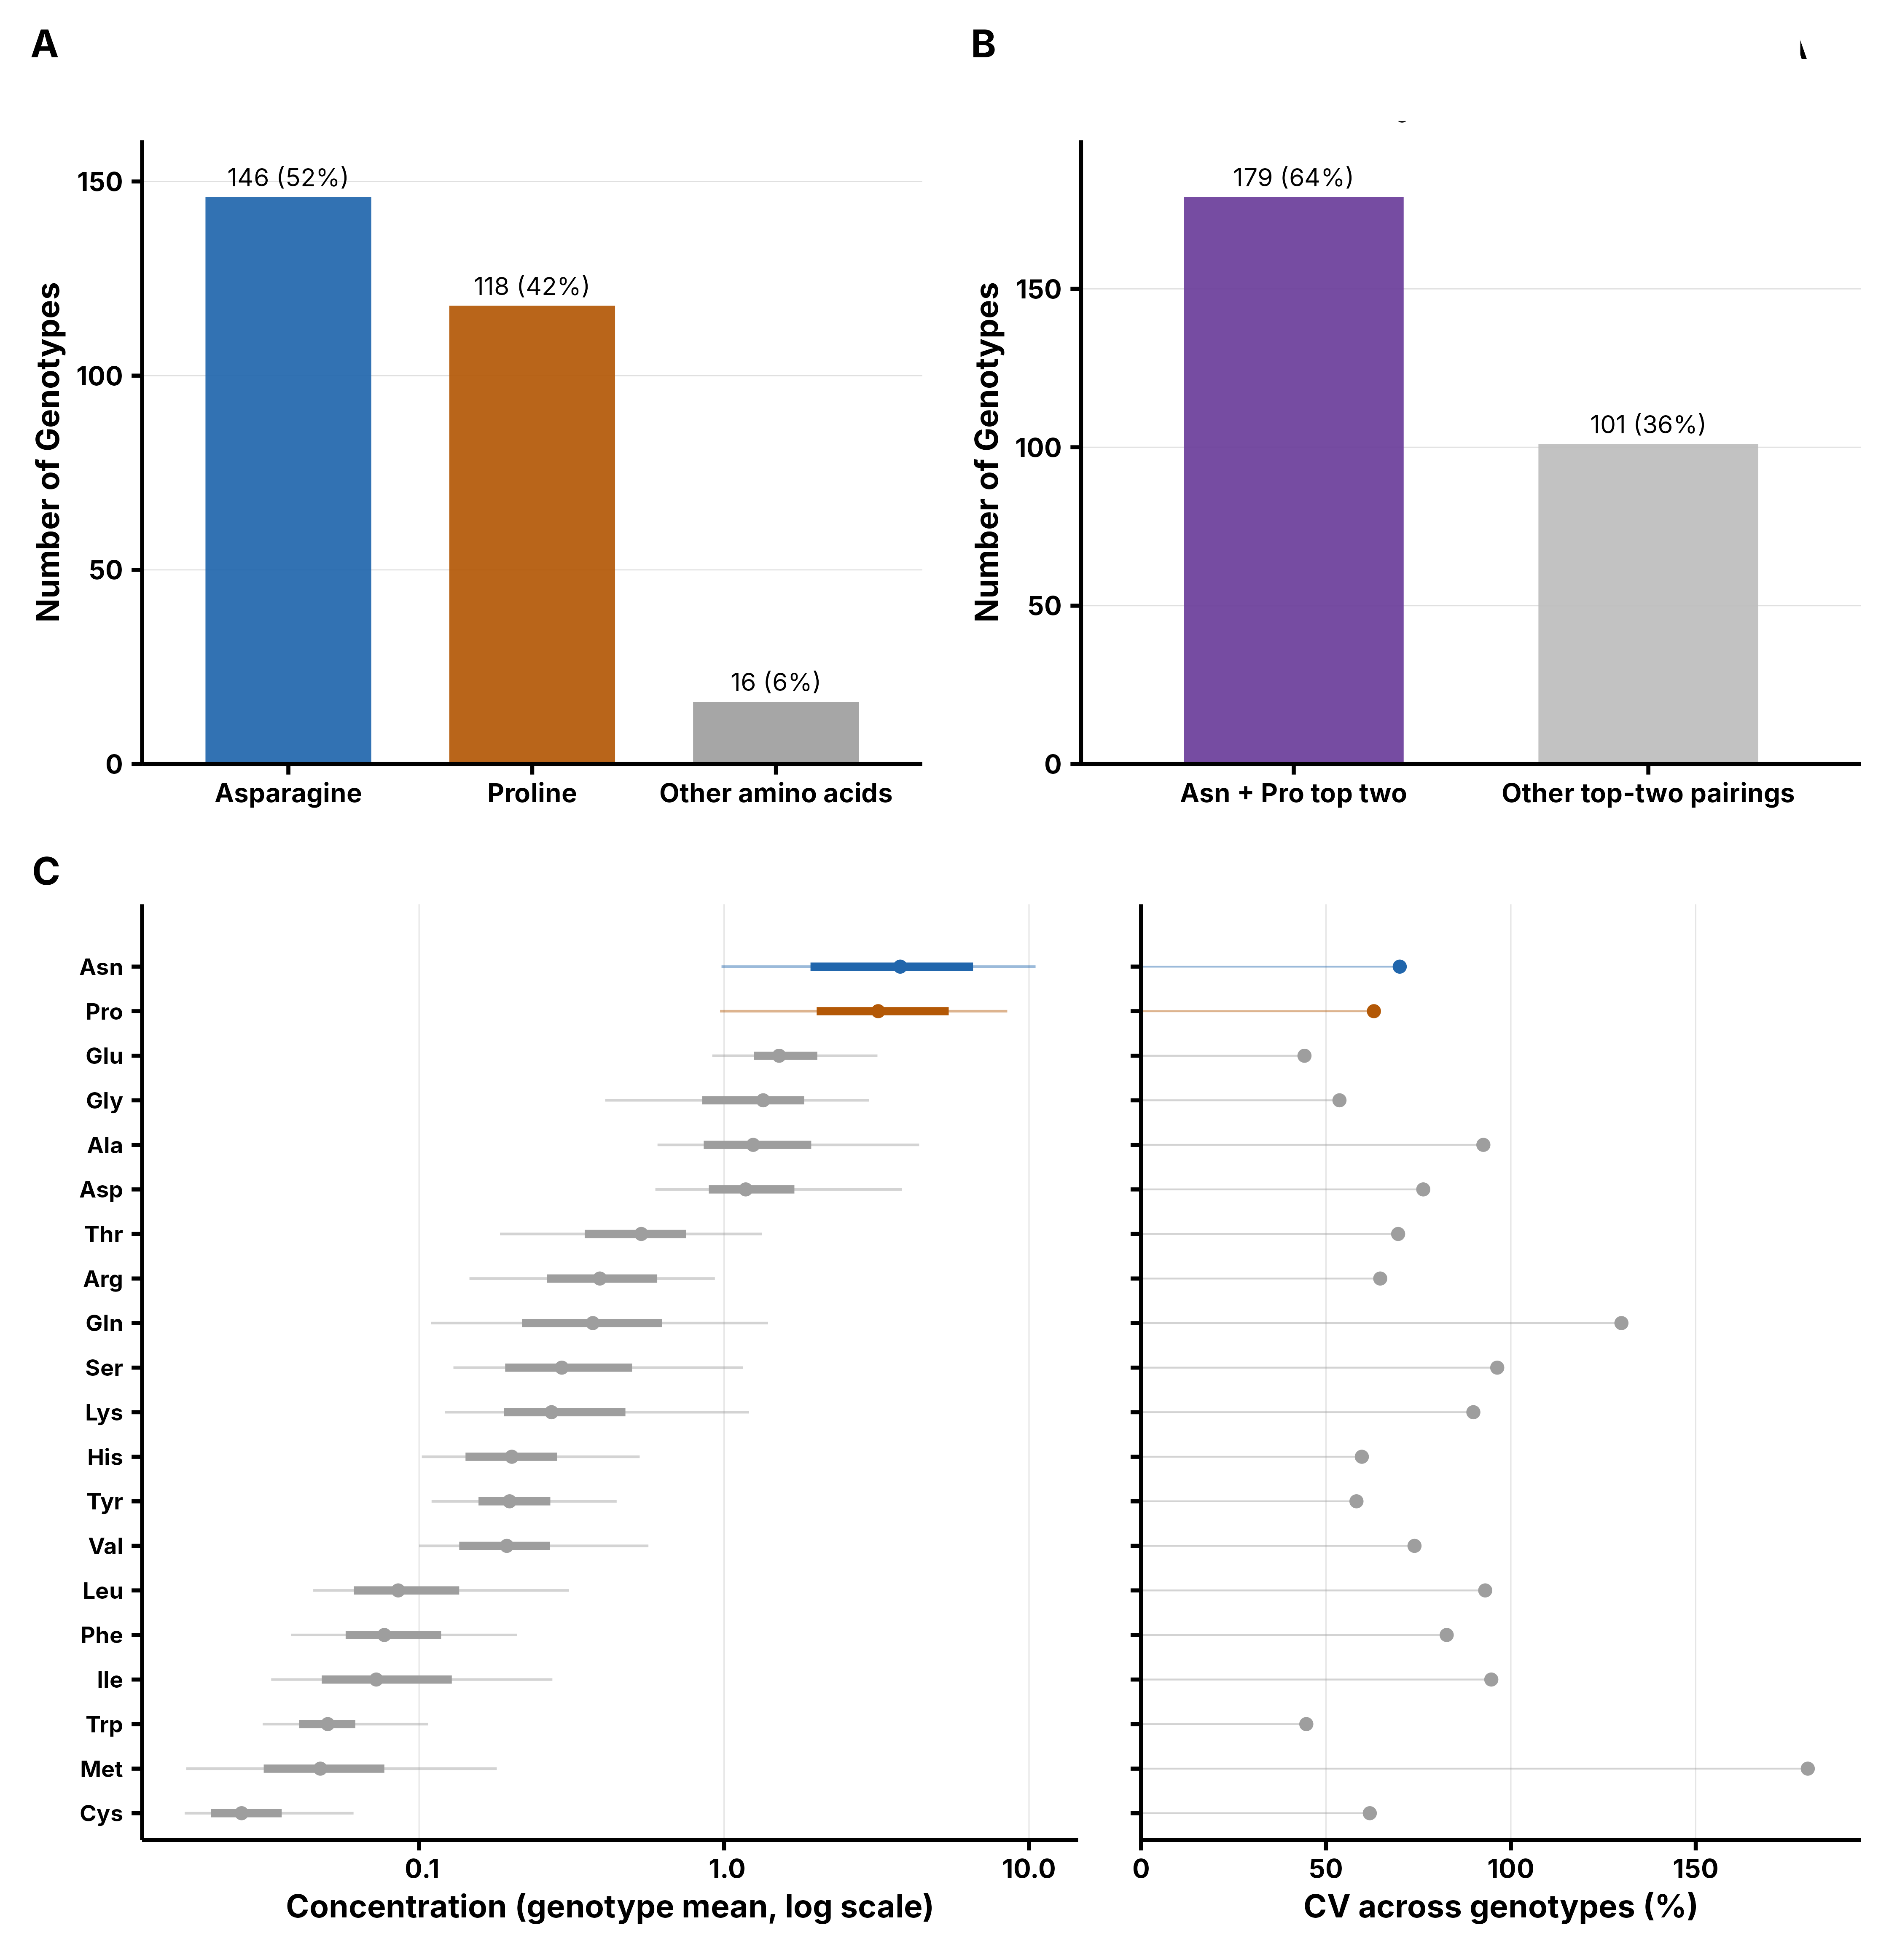
\includegraphics[width=0.95\textwidth]{final/supp_figs/SuppFig1_FAA_composition.png}
    \caption{Free amino acid composition of the Goodman--Buckler panel.
    \textbf{A}, Number of genotypes in which each free amino acid ranked most abundant,
    based on genotype means across four replicates ($n = 280$ genotypes).
    \textbf{B}, Number of genotypes in which asparagine and proline together occupied the
    top two ranks, in either order.
    \textbf{C}, Abundance and variability of each free amino acid. Left, concentration per
    genotype mean on a log scale: point, median across genotypes; thick bar, interquartile
    range; thin bar, 5th--95th percentile; amino acids ordered by median. Right,
    coefficient of variation across genotypes for the same ordering. Median concentrations
    span 144-fold between the most and least abundant amino acids. Abundance and
    variability are not equivalent orderings: methionine is both the least abundant amino
    acid and the most variable (CV 180\%), whereas asparagine and proline are comparatively
    stable (CV 70\% and 63\%). Asparagine is shown in blue and proline in orange
    throughout.}
    \label{fig:supp_faa_asn_pro_rank}
\end{figure*}

% =========================
% SUPP FIGURE S2
% =========================  

\begin{figure*}[ht!]
    \centering
    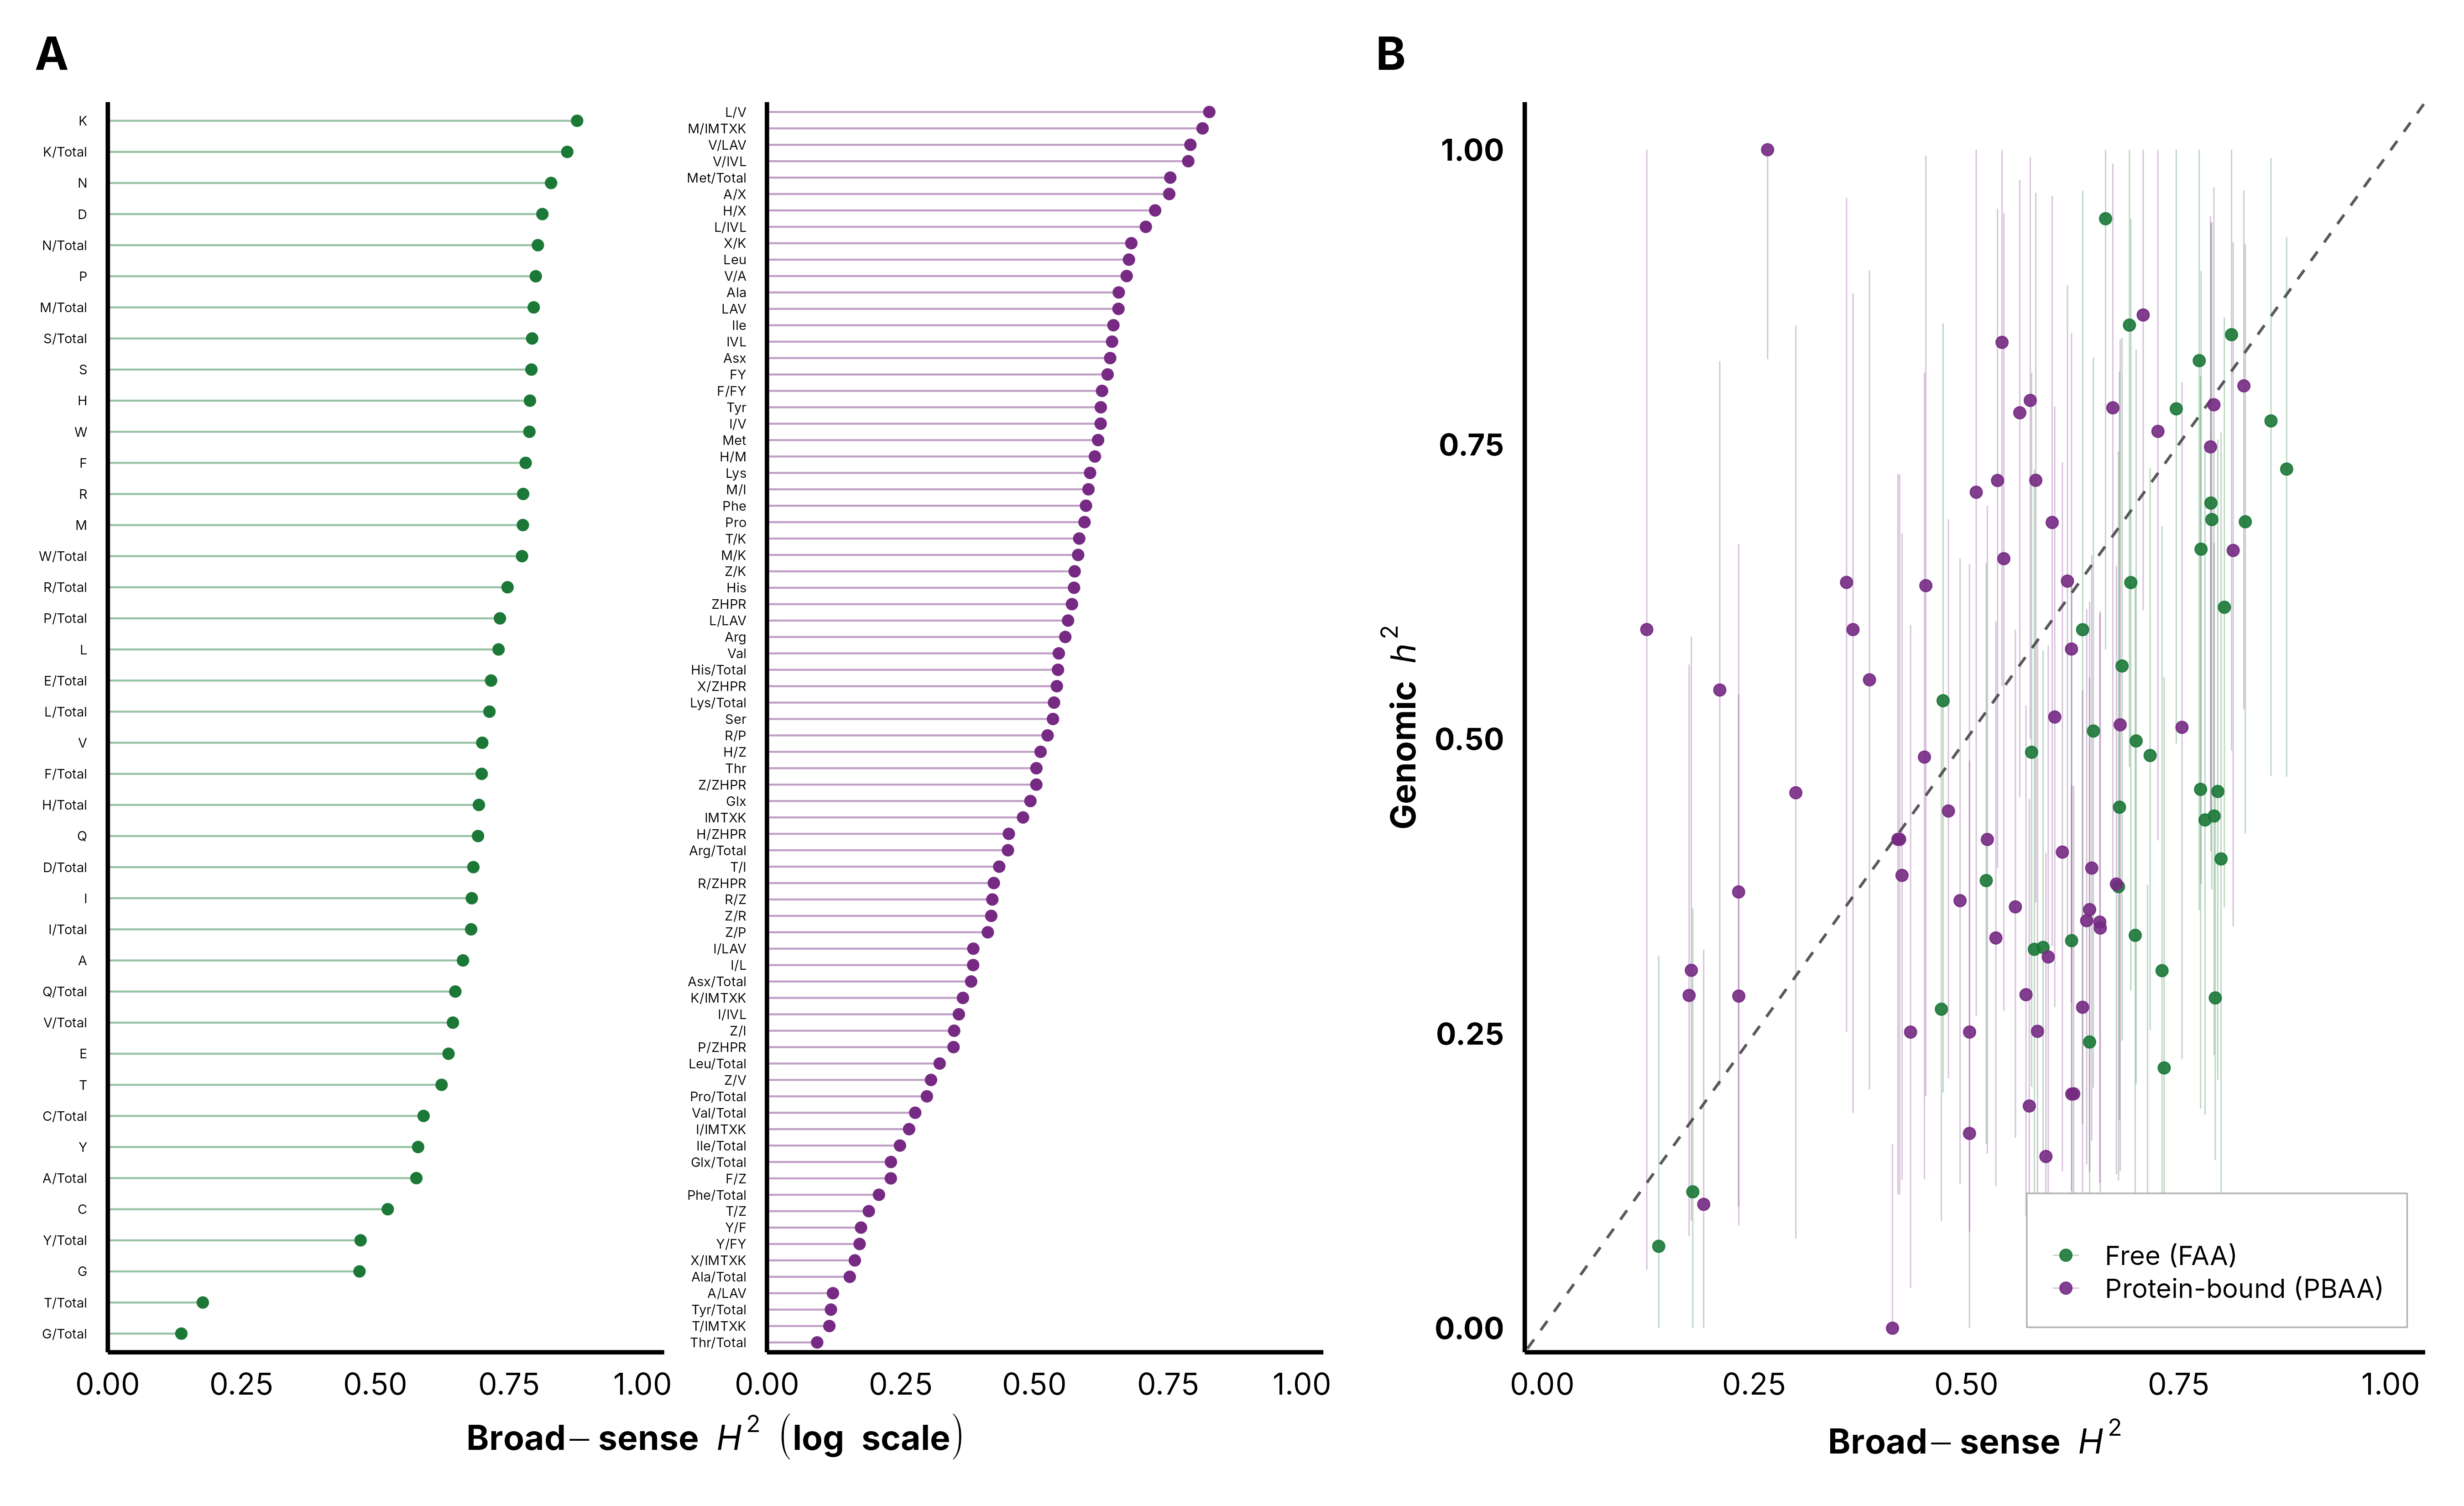
\includegraphics[width=\textwidth]{final/supp_figs/SuppFig2_heritability.png}
    \caption{Heritability of grain amino acid phenotypes in the Goodman--Buckler panel.
    \textbf{A}, Broad-sense heritability $H^2$ on a line-mean basis, estimated on the log
    scale from the raw plot records (two years $\times$ two blocks) with the model
    $y \sim 1 + (1|\mathrm{taxa}) + (1|\mathrm{year}) + (1|\mathrm{taxa{:}year}) +
    (1|\mathrm{year{:}block})$, shown for 40 free and 76 protein-bound amino acid traits.
    The Cullis generalized $H^2$ agrees with the line-mean estimate to within 0.018 across
    every trait and is not shown separately. \textbf{B}, Genomic heritability $h^2$ from a
    VanRaden genomic relationship matrix plotted against $H^2$, with error bars giving the
    95\% profile-likelihood interval on $h^2$ and the dashed line showing $y = x$. Because
    $H^2$ is estimated from approximately 1{,}000 plot records and $h^2$ from 272
    genotypes, the $h^2$ intervals are wide (median width 0.52) and point estimates cross
    the line freely; $H^2$ falls within the $h^2$ interval for 73\% of traits. Fifteen of
    116 traits returned a non-zero $h^2$ from a permuted phenotype and are excluded from
    panel \textbf{B}; their $H^2$ is unaffected and is retained in panel \textbf{A}.}
    \label{fig:supp_heritability}
\end{figure*}

% =========================
% SUPP FIGURE S3
% =========================
\begin{figure*}[ht!]
    \centering
    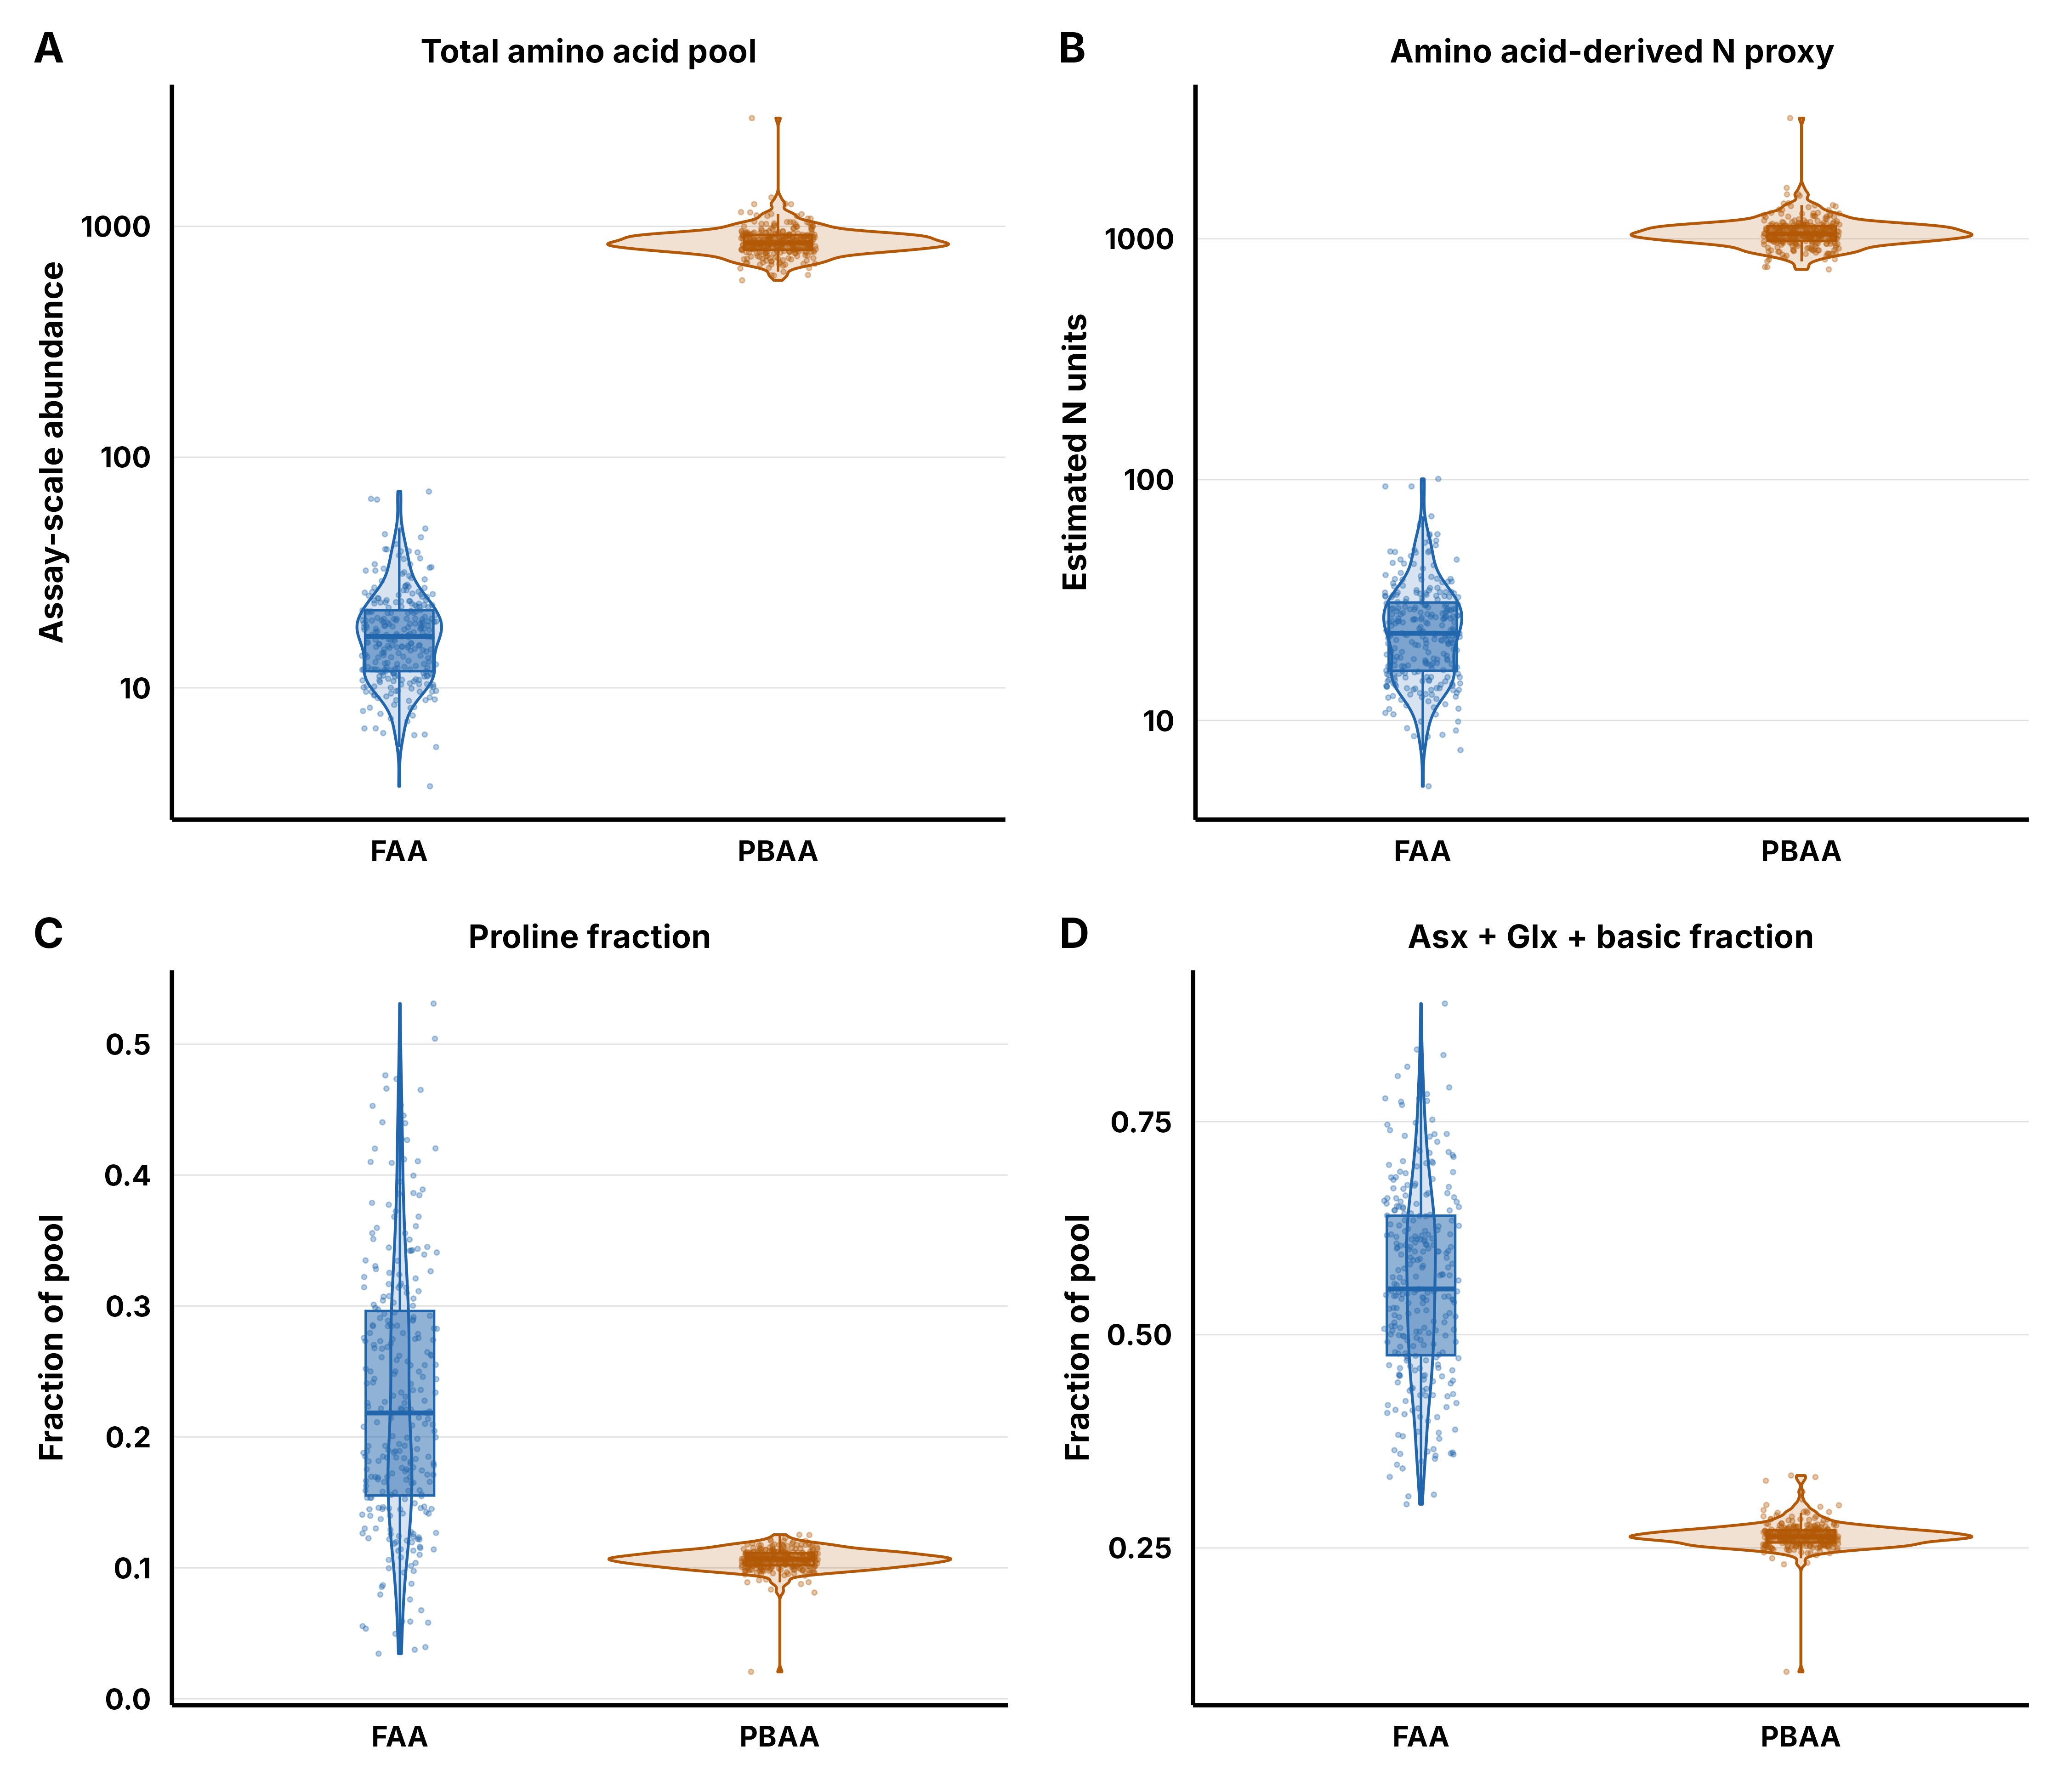
\includegraphics[width=\textwidth]{final/supp_figs/SuppFig3_FAA_vs_PBAA_pools.png}
    \caption{Free (FAA) and protein-bound (PBAA) amino acid pools across matched Goodman--Buckler
    lines ($n = 279$). \textbf{A}, Total amino acid pool. \textbf{B}, Amino acid-derived N proxy,
    with each amino acid weighted by its number of N atoms (Asx and Glx, unresolved after acid
    hydrolysis, at 1.5 N). \textbf{C}, Proline fraction. \textbf{D}, Asx + Glx + basic
    (Arg, Lys, His) fraction. Fractions use matched denominators: free Asp + Asn and Glu + Gln
    are combined, and glycine, tryptophan and cysteine, which are not measured in the
    protein-bound pool, are excluded from the free-pool total. Values are on the source assay
    scale (log scale in \textbf{A}--\textbf{B}). Violins show the distribution across lines and
    boxes the median and interquartile range. Paired Wilcoxon signed-rank tests are given in
    Supplementary Table~S5.}
    \label{fig:supp_gb_faa_pbaa_metrics}
\end{figure*}

% =========================
% SUPP FIGURE: chromosome 9 amino acid GWAS locus
% =========================
\begin{figure*}[ht!]
    \centering
    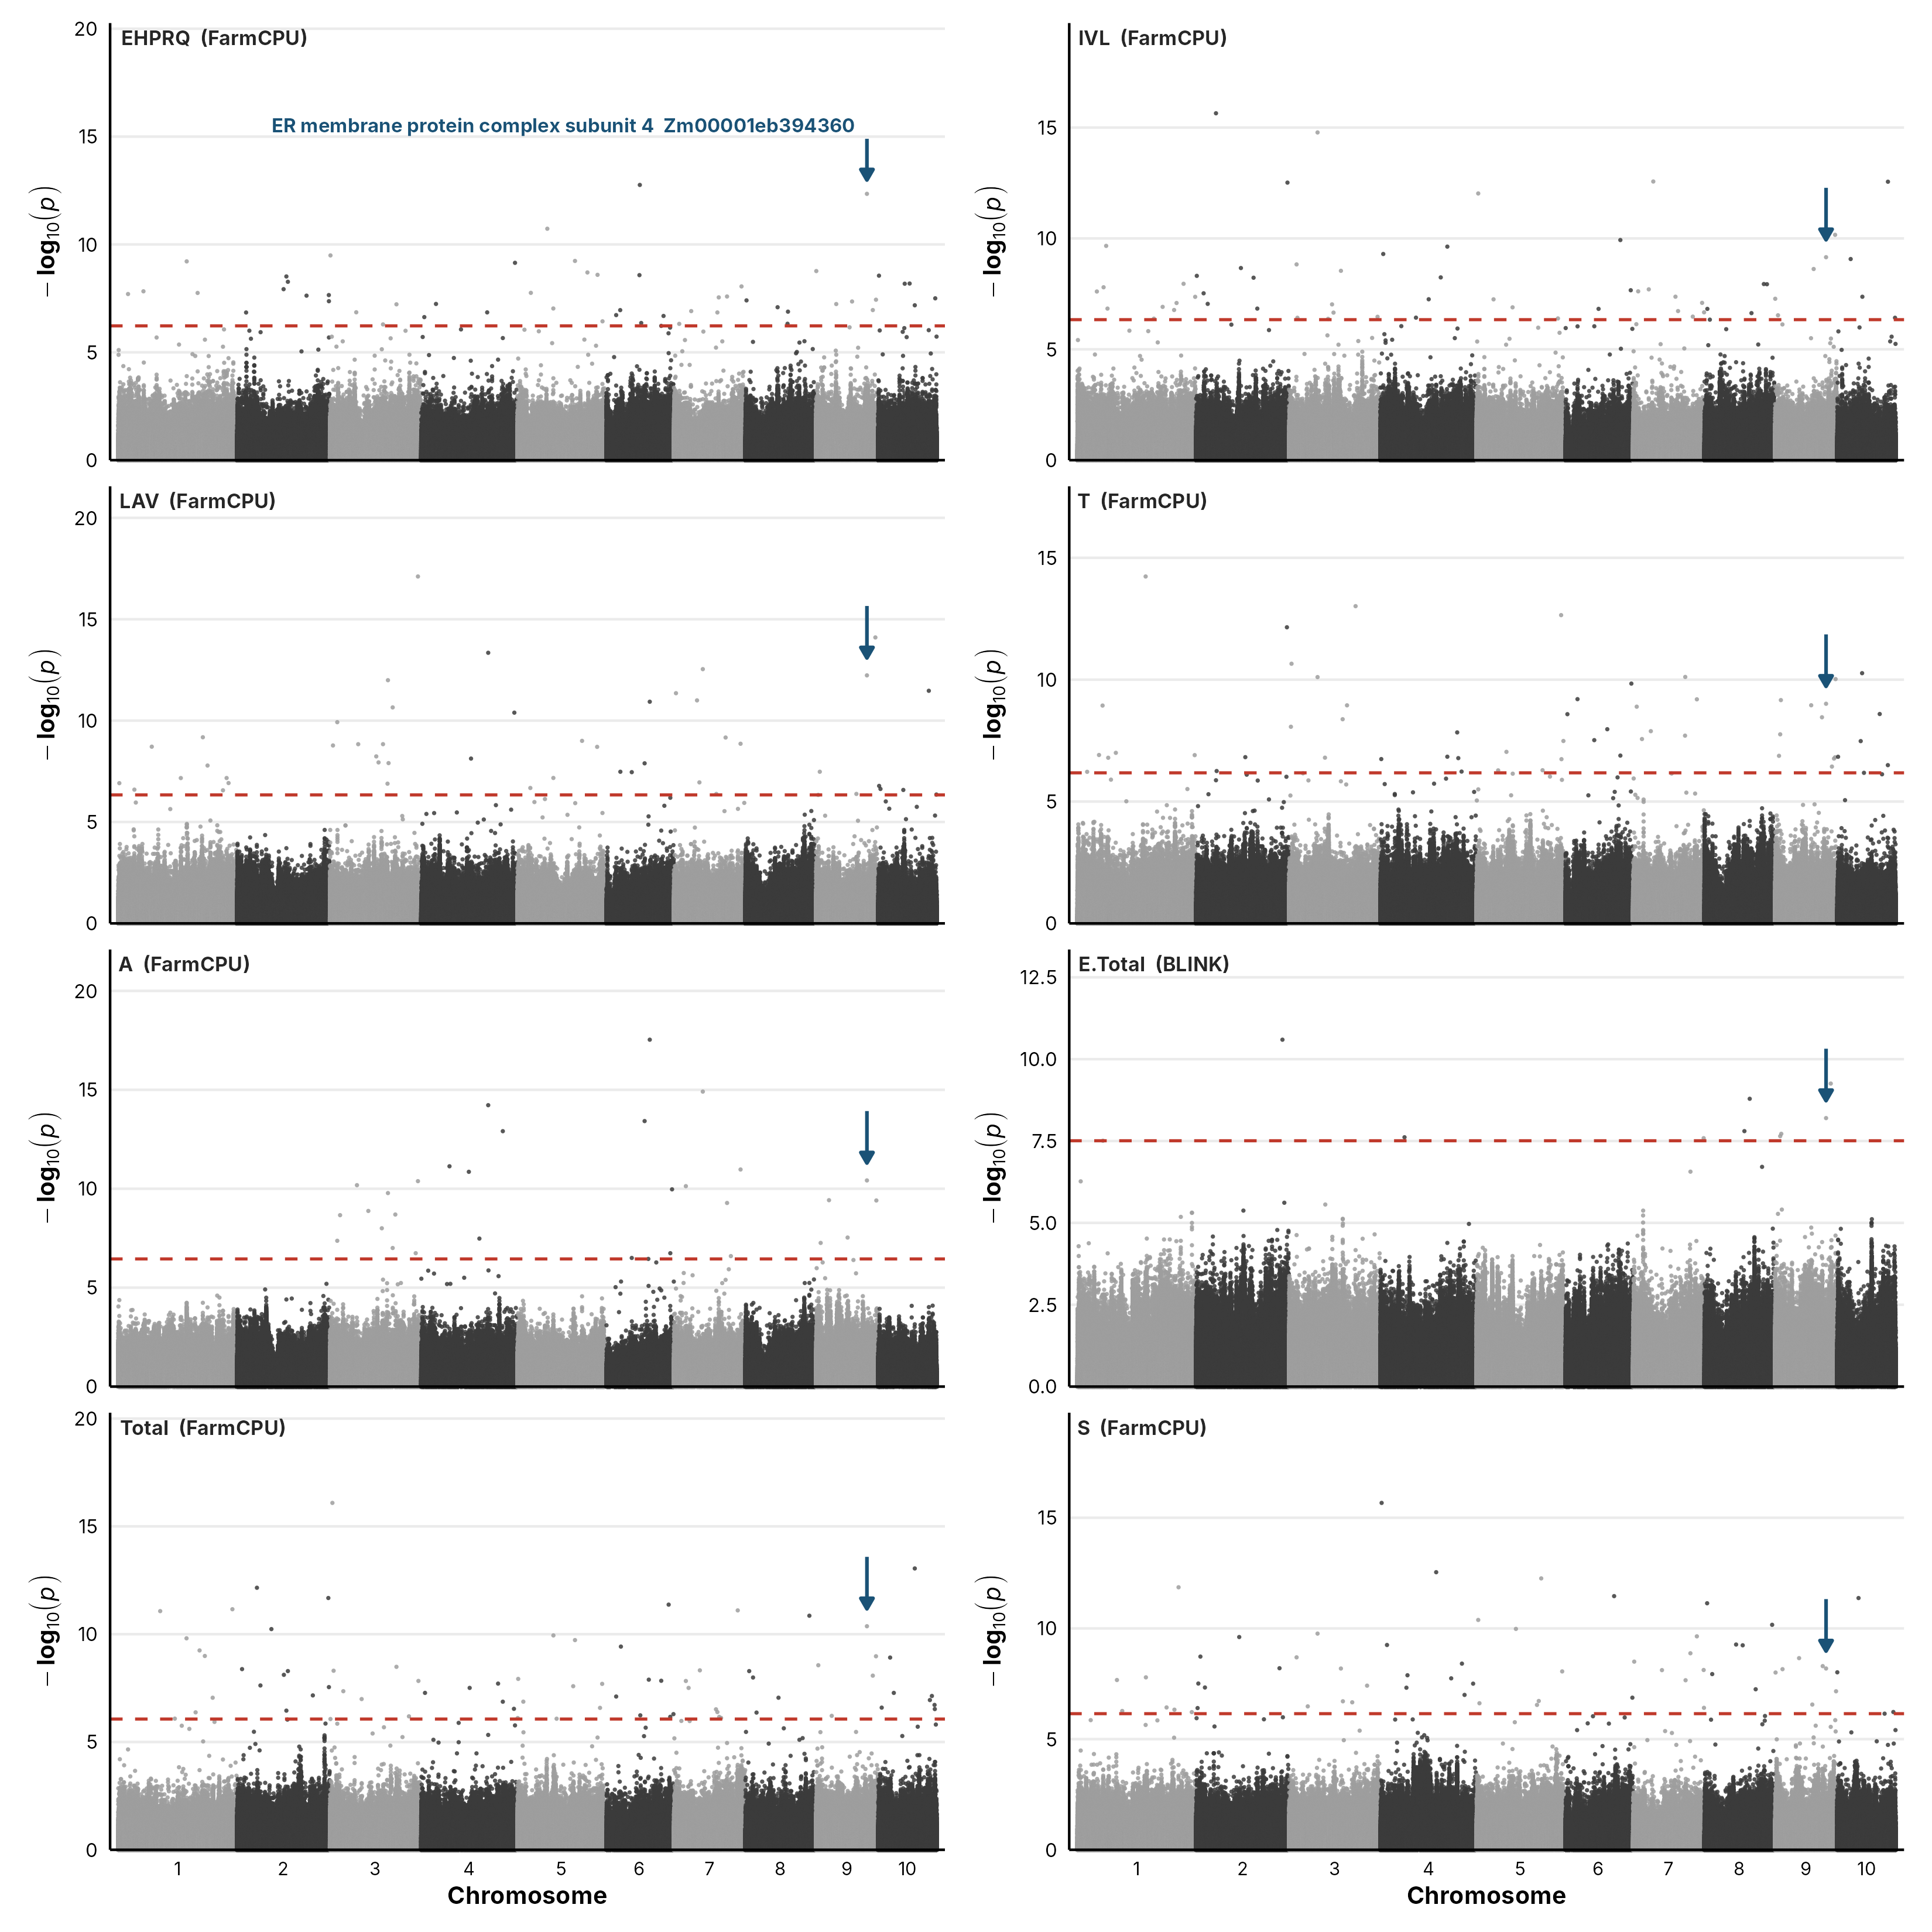
\includegraphics[width=0.82\textwidth]{final/supp_figs/SuppFig_amino_chr9_locus_manhattan.png}
    \caption{A locus on chromosome 9 associated with nine amino acid phenotypes. Manhattan plots for eight phenotypes with an FDR-significant association near \textit{Zm00001eb394360} (ER membrane protein complex subunit 4; chr9:133,919,123--133,923,877); \textit{N.E} ($P = 1.1 \times 10^{-7}$) is omitted. The associations form three groups: four SNPs in strong linkage disequilibrium ($r^2 = 0.79$--$0.94$), spanning 13 kb from the 3$'$ end of \textit{Zm00001eb394360} to the 5$'$ end of \textit{Zm00001eb394380} (rhomboid-like protein 19), significant for \textit{A}, \textit{LAV}, \textit{IVL}, \textit{T}, \textit{S}, \textit{Total} and \textit{E.Total}; and two SNPs unlinked to them ($r^2 \le 0.12$), significant for \textit{EHPRQ} and \textit{N.E}. All SNPs are plotted at B73 RefGen\_v5 positions lifted from AGPv4. Arrows mark the lead SNP within 250 kb of the gene. Dashed red lines indicate the 5\% Benjamini--Hochberg FDR threshold (cutoffs $P = 8.6 \times 10^{-7}$ to $3.1 \times 10^{-8}$). The model for each phenotype is in parentheses.}
    \label{fig:supp_amino_chr9_locus}
\end{figure*}


% =========================
% SUPP FIGURE S4
% =========================                                                    

\begin{figure}[htbp]
  \centering
  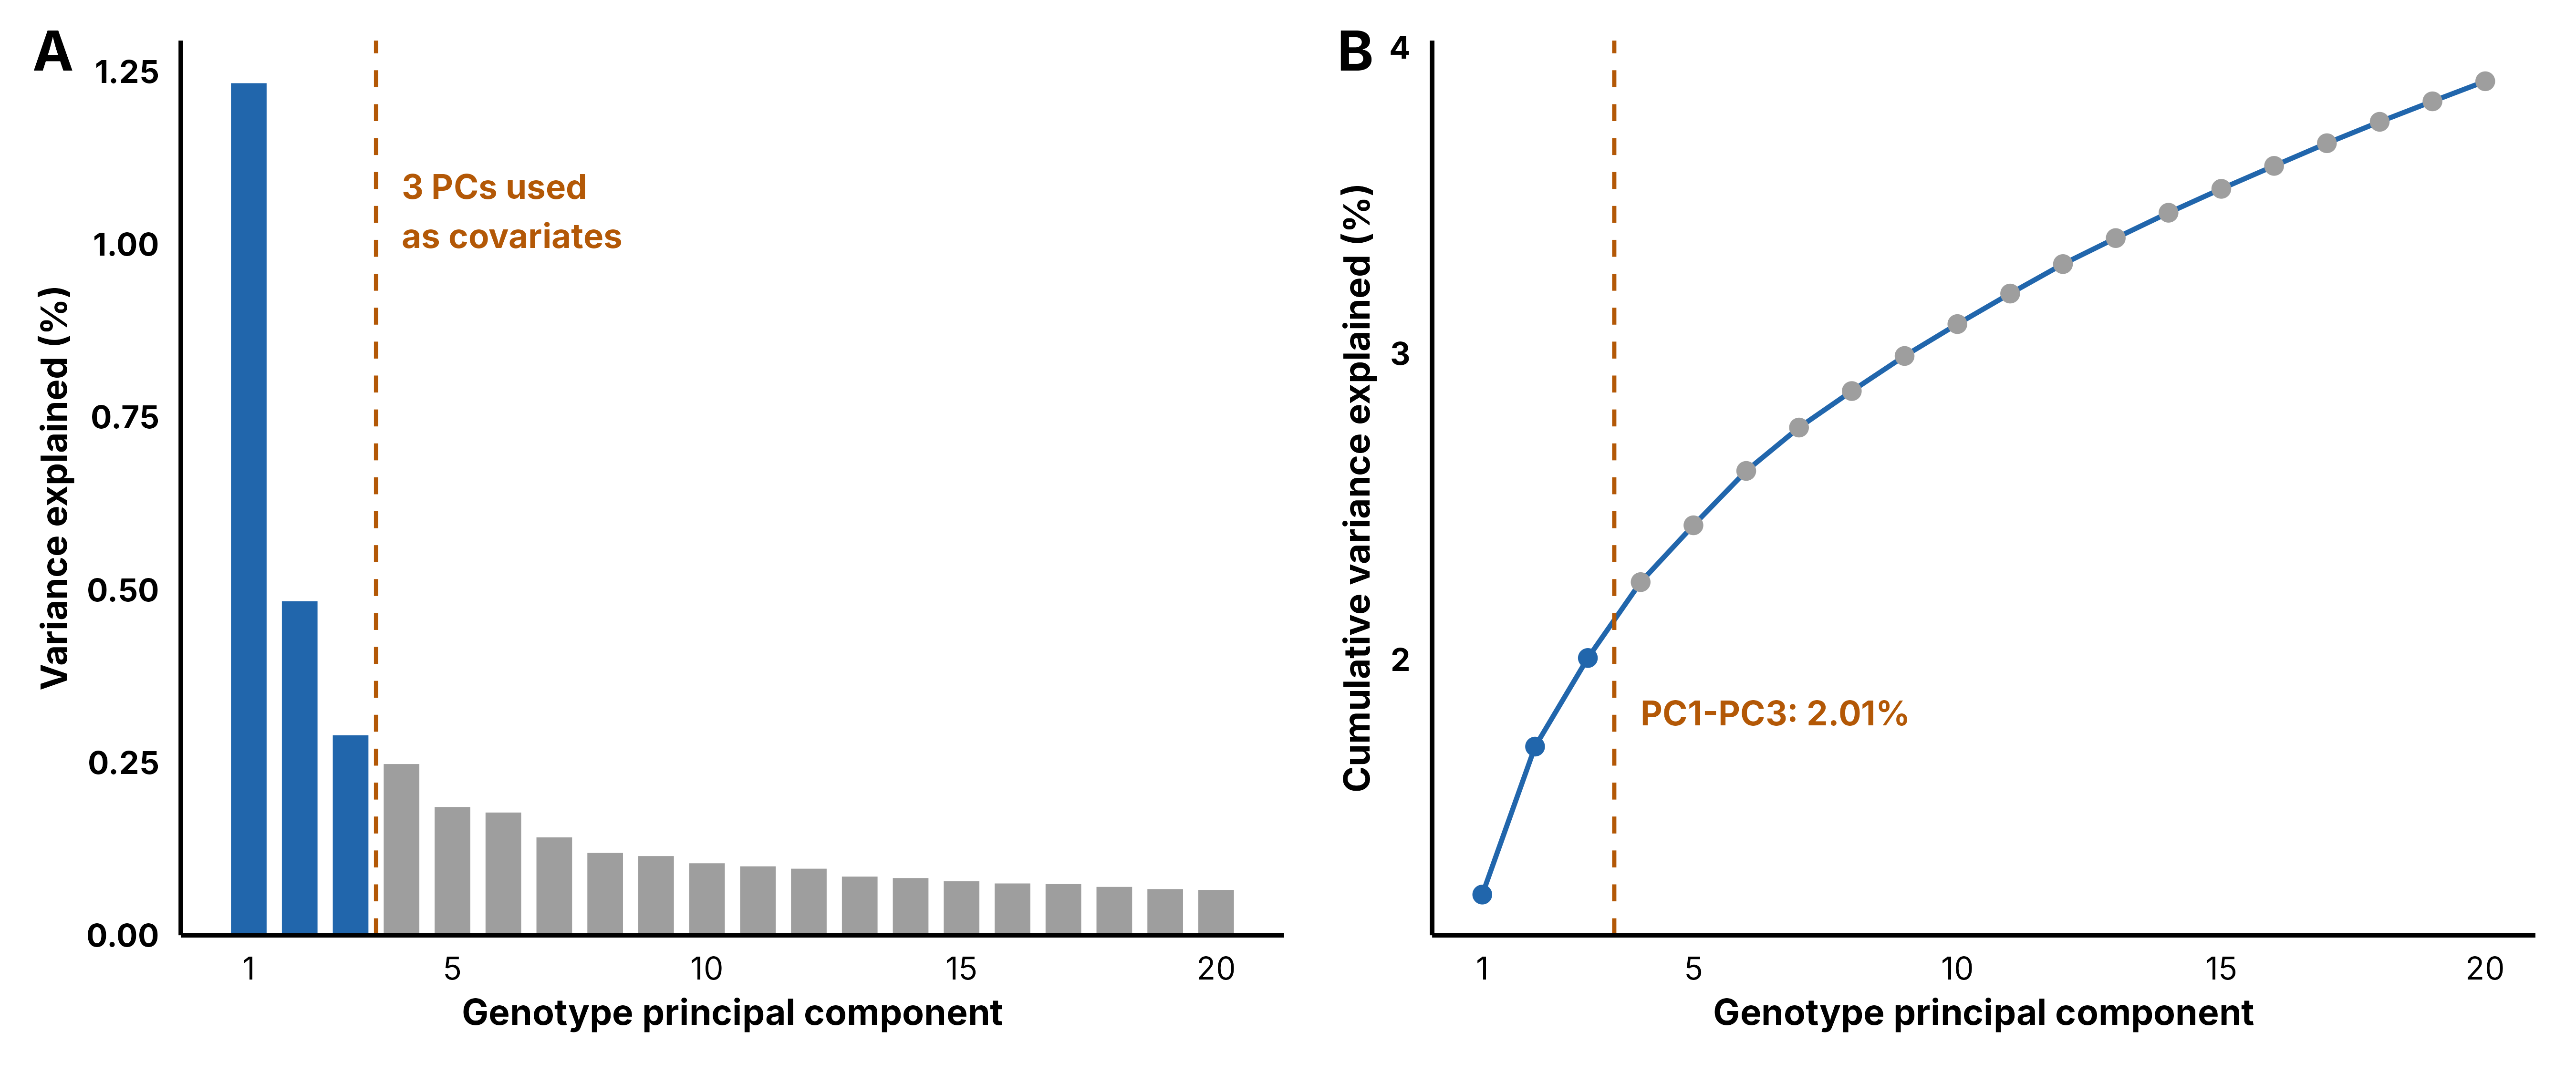
\includegraphics[width=\textwidth]{final/supp_figs/SuppFig_genotype_PCA_scree.png}
  \caption{\textbf{Genotype principal components of the landrace panel.}
  \textbf{(A)} Variance explained by each of the first 20 PCs.
  \textbf{(B)} Cumulative variance explained. The last large drop is from PC2 to PC3;
  after PC3, each further PC explains $\leq 0.06$ percentage points less than the one before.
  The first three PCs (blue; 2.01\% of variance) were used as GWAS covariates.}
  \label{fig:supp_pca_scree}
\end{figure}

% =========================
% SUPP FIGURE S5
% =========================
\begin{figure}[htbp]
  \centering
  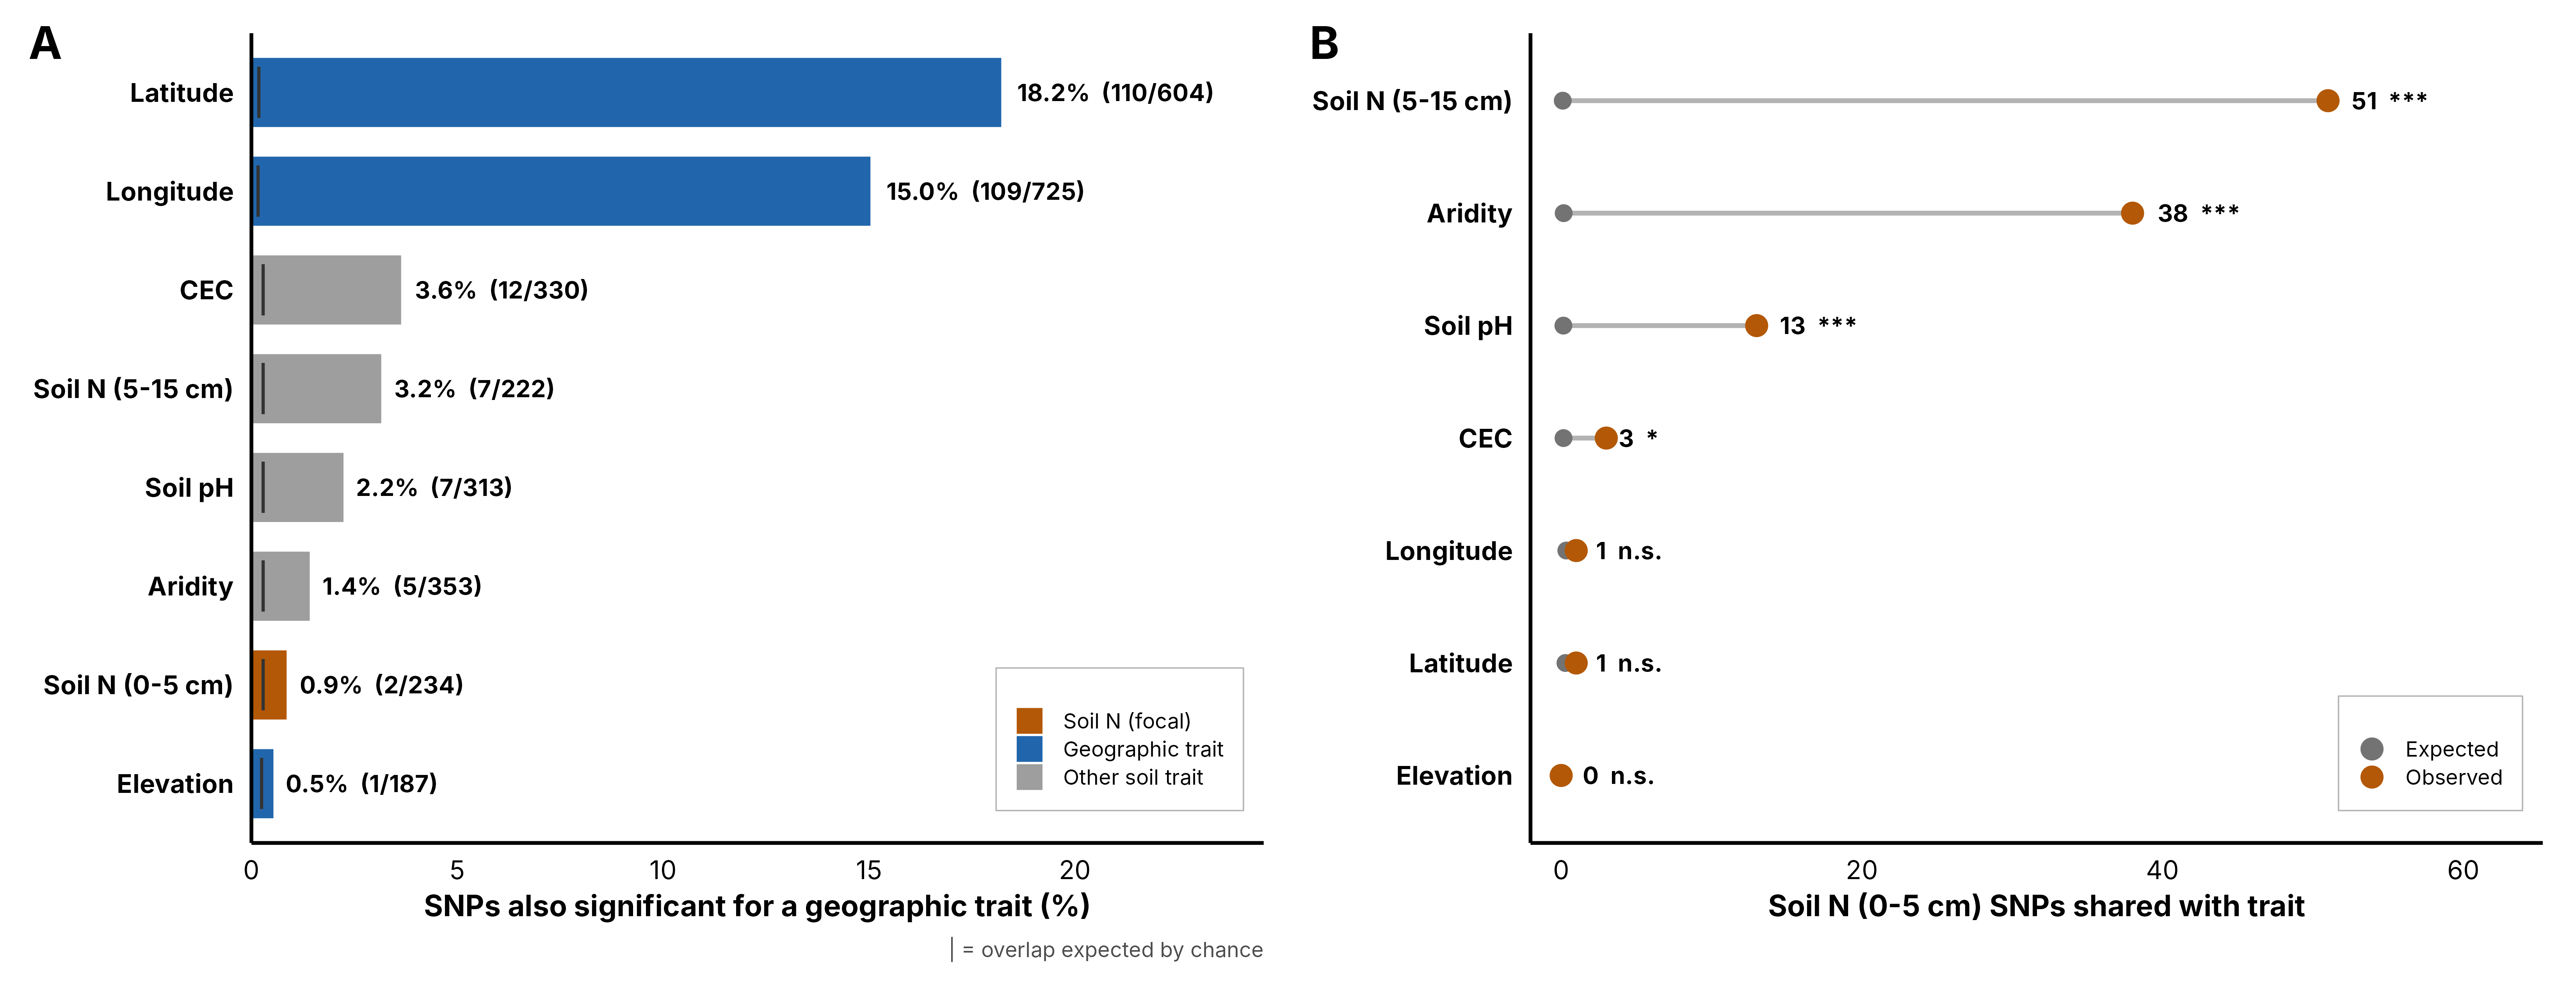
\includegraphics[width=\textwidth]{final/supp_figs/SuppFig_soilN_specificity.png}
  \caption{\textbf{Overlap of soil-N associations with other environmental GWAS.}
  Each variable was scanned with MLM, BLINK and FarmCPU (3 PCs, 495,755 SNPs); a SNP counts as
  significant for a variable if it reaches 5\% FDR in any model.
  \textbf{(A)} Percentage of each variable's significant SNPs that are also significant for a
  geographic variable (latitude, longitude, elevation; the variable itself excluded). Vertical
  ticks, percentage expected by chance.
  \textbf{(B)} SNPs shared between soil N (0--5~cm) and each other variable: observed (orange)
  vs.\ expected (grey). One-sided hypergeometric test, $M = 495{,}755$:
  *\,$P<0.05$; **\,$P<10^{-5}$; ***\,$P<10^{-20}$; n.s., not significant.
  Full results in Supplementary Table~S9.}
  \label{suppfig:soilN_specificity}
\end{figure}


% =========================
% SUPP FIGURE S6
% =========================                                                    

\begin{figure}[htbp]
  \centering
  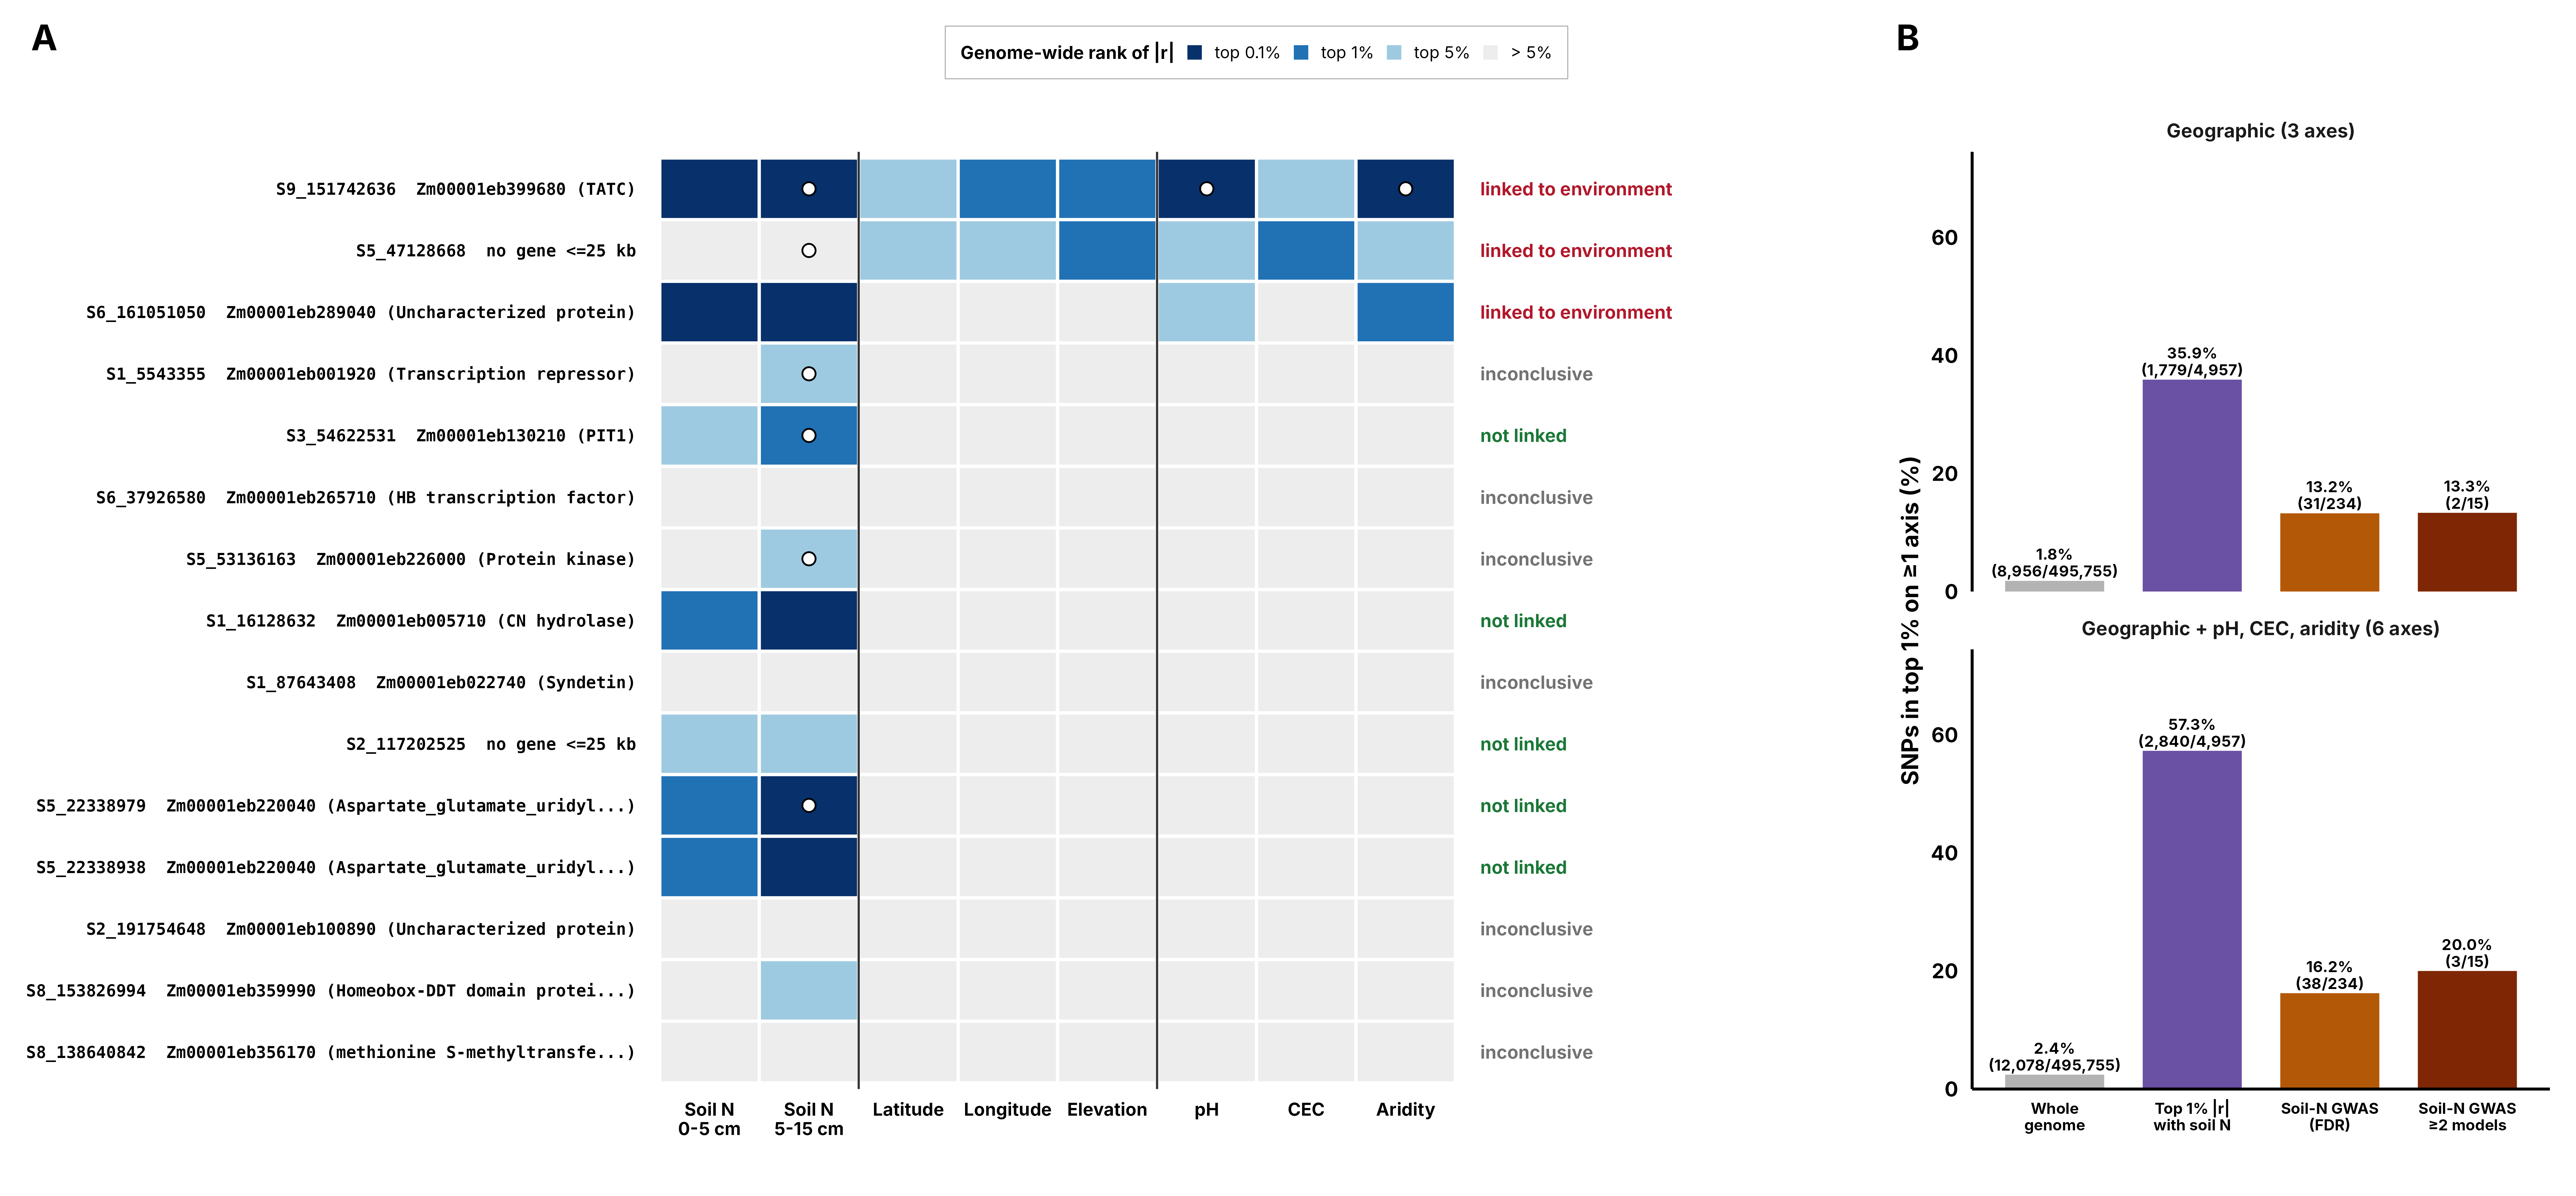
\includegraphics[width=\textwidth]{final/supp_figs/SuppFig_soilN_geno_env_correlation.png}
  \caption{\textbf{Genotype--environment correlation test for the soil-N SNPs.}
  For each of 495,755 SNPs, we computed the Pearson correlation ($r$) between the SNP's genotype
  (0, 1 or 2 copies of the allele) and each site variable across 3,107 accessions, then ranked
  every SNP against the whole genome by $|r|$ (e.g.\ ``top 1\%'' = fewer than 1\% of SNPs
  correlate more strongly with that variable).
  \textbf{(A)} The 15 soil-N SNPs significant in at least two GWAS models. Tile colour shows the
  genome-wide rank of each SNP's correlation with each variable. Open circles mark SNPs that were
  also significant (5\% FDR) in that variable's own GWAS. Each SNP's call is shown on the right:
  \textit{linked to environment}, its genotype is in the top 1\% of the genome for correlation
  with at least one non-N variable, so its soil-N association cannot be separated from geography
  or climate;
  \textit{not linked}, its genotype correlates strongly with soil N (top 5\%) but not with any
  other variable;
  \textit{inconclusive}, its genotype correlates only weakly with soil N across all accessions
  (outside the top 5\%), so there is no soil-N correlation to compare the other variables
  against. These SNPs were detected only by BLINK and FarmCPU, which test each SNP after
  accounting for population structure and other strongly associated SNPs; this test applies no
  such adjustment and therefore cannot judge them in either direction.
  \textbf{(B)} Expectation test: percentage of SNPs whose genotype is in the top 1\% for at least
  one geographic variable (latitude, longitude, elevation; top) or for at least one of all six
  non-N variables (bottom), for the whole genome, for SNPs in the top 1\% for correlation with
  soil N, and for the soil-N GWAS SNPs. Full results in Supplementary Tables~S11--S12.}
  \label{suppfig:soilN_geno_env}
\end{figure}







% =========================
% SUPP FIGURE S7
% =========================
\begin{figure*}[htbp]
\centering
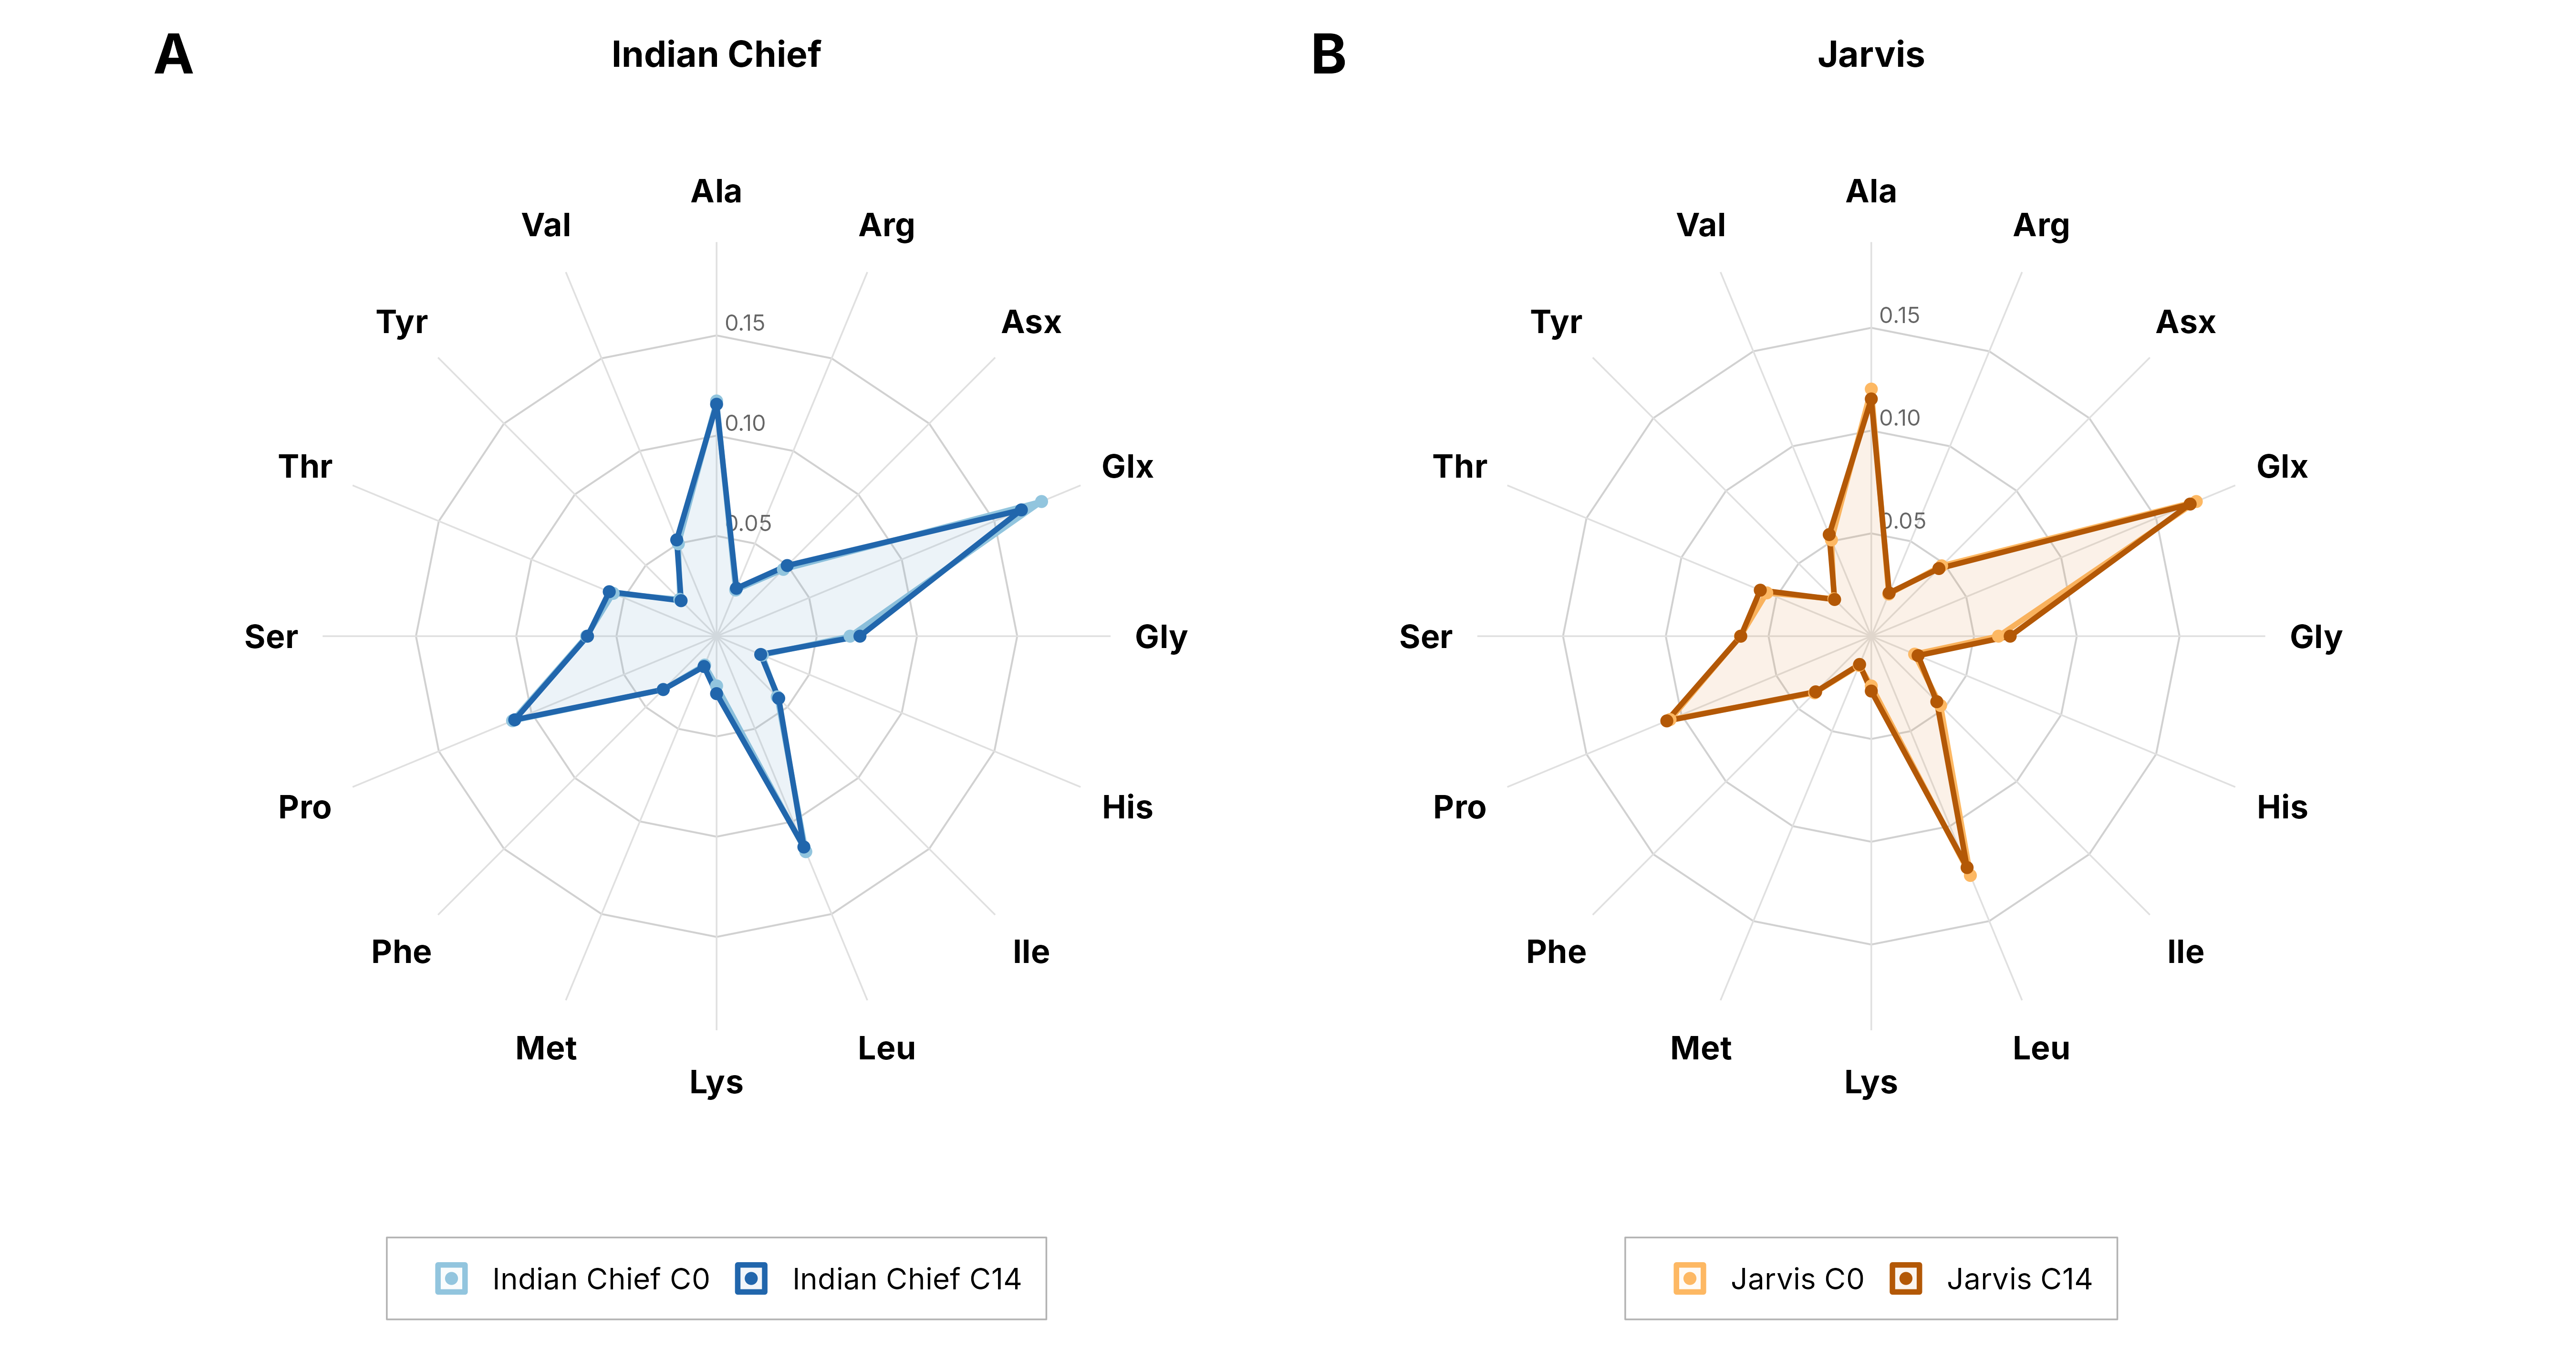
\includegraphics[width=\textwidth]{final/supp_figs/SuppFig_IC_J_PBAA_composition.png}
\caption{
\textbf{Protein-bound amino acid (PBAA) composition in Indian Chief and Jarvis at Cycle~0 (C0) and Cycle~14 (C14).} Mean fraction of each of 16 protein-bound amino acids in the total PBAA pool, averaged over biological samples (Indian Chief C0 $n = 5$, C14 $n = 8$; Jarvis C0 $n = 3$, C14 $n = 8$), for \textbf{(A)} Indian Chief and \textbf{(B)} Jarvis. Asx and Glx are the combined Asp + Asn and Glu + Gln pools after acid hydrolysis; tryptophan and cysteine are not measured. Rings mark fractions of 0.05, 0.10 and 0.15. No amino acid differed between cycles in either population (two-sided Wilcoxon rank-sum tests, Benjamini--Hochberg-adjusted across the 16 amino acids; Supplementary Table~S14).
}
\label{fig:supp_pbaa_profiles}
\end{figure*}

% =========================
% SUPP FIGURE S8
% =========================
\begin{figure*}[htbp]
\centering
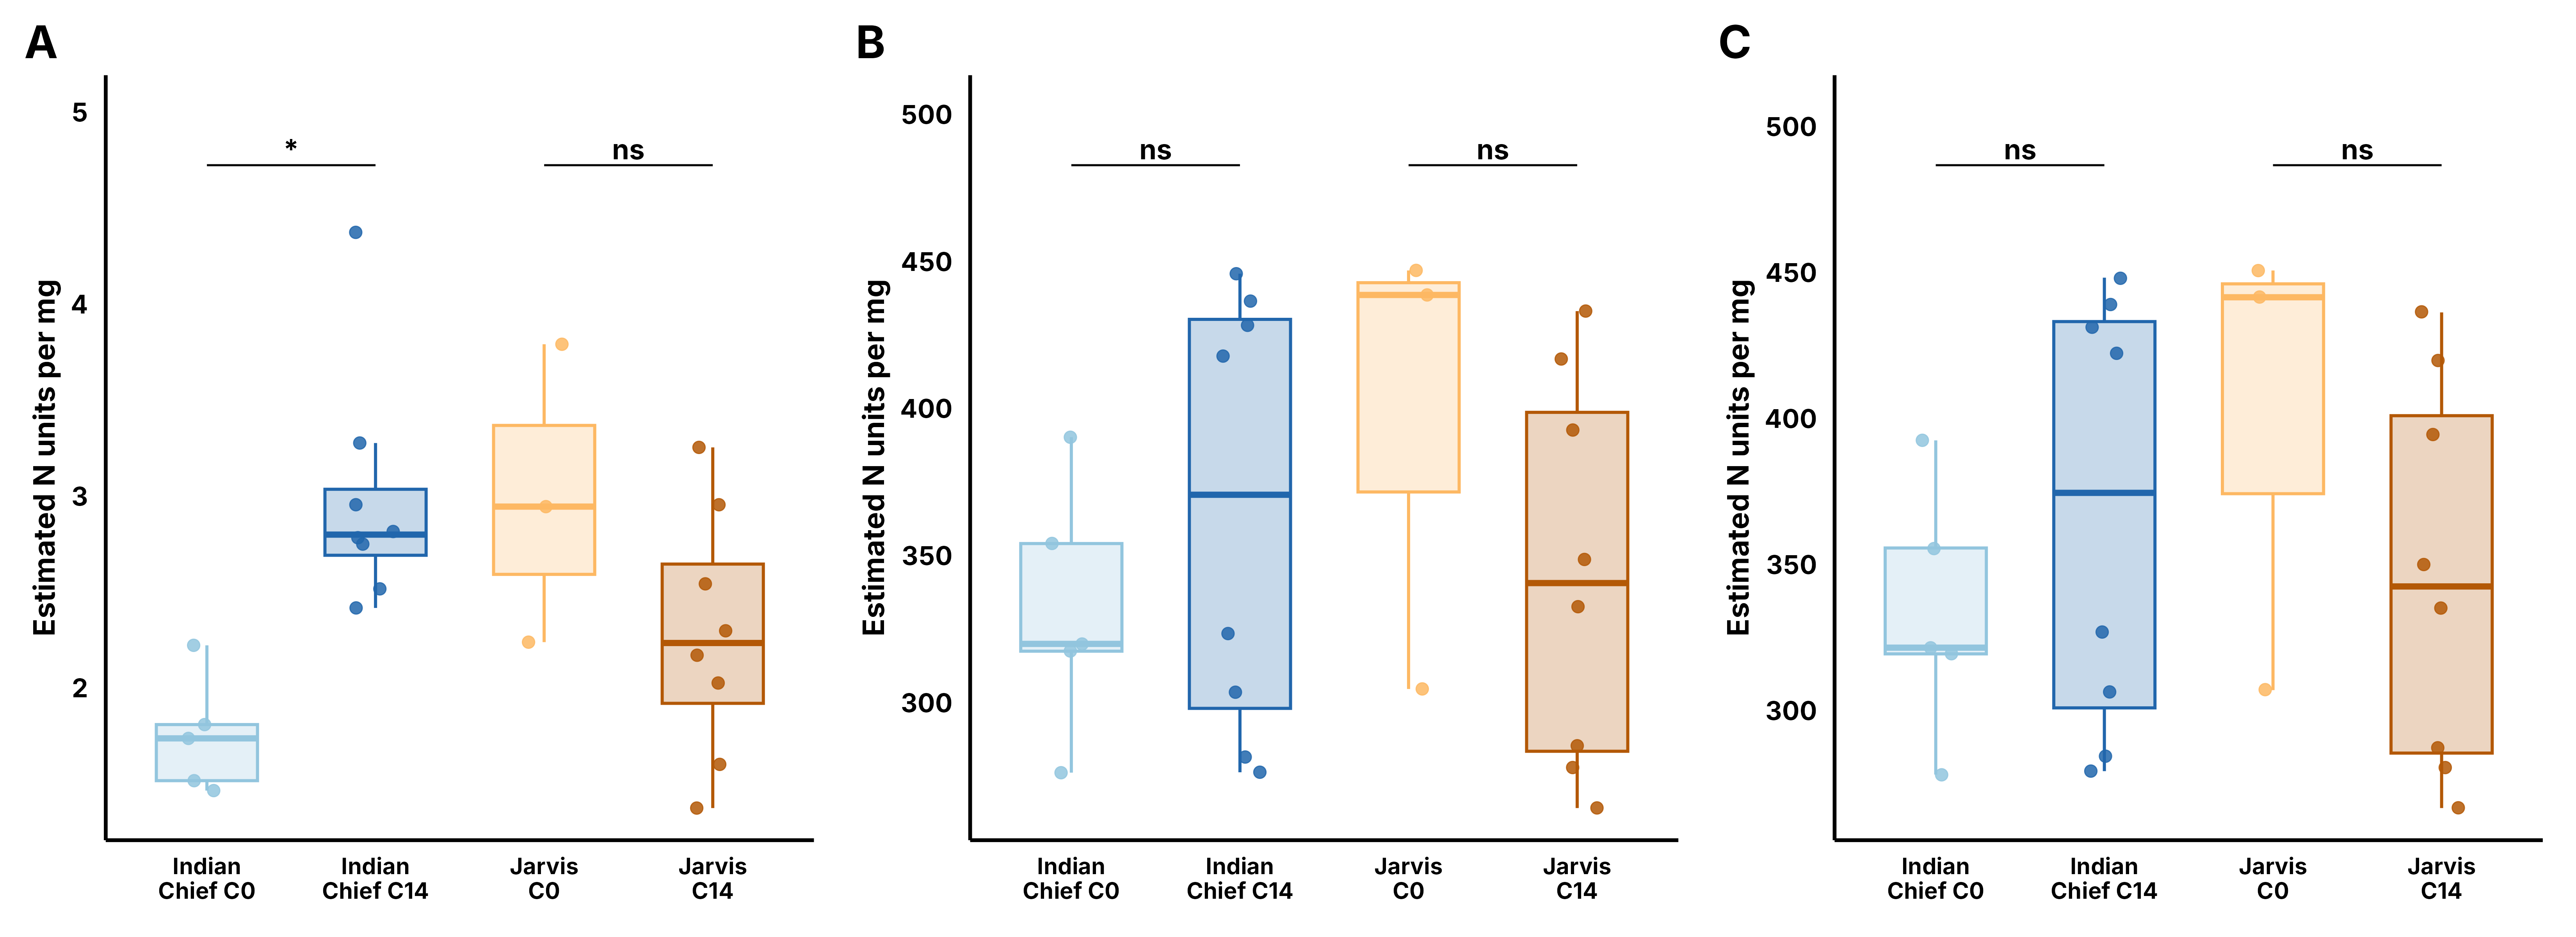
\includegraphics[width=\textwidth]{final/supp_figs/SuppFig_IC_J_AA_N_pools.png}
\caption{
\textbf{Amino acid-derived nitrogen per mg sample in Indian Chief and Jarvis at Cycle~0 (C0) and Cycle~14 (C14).} \textbf{(A)} FAA-derived N, \textbf{(B)} estimated protein-bound amino acid-derived N and \textbf{(C)} estimated total amino acid-derived N (A + B). Each amino acid was weighted by its number of N atoms (Arg 4; His 3; Asn, Gln, Lys and Trp 2; all others 1; protein-bound Asx and Glx 1.5) and divided by sample mass. Points are biological samples (Indian Chief C0 $n = 5$, C14 $n = 8$; Jarvis C0 $n = 3$, C14 $n = 8$); boxes show the median and interquartile range. Brackets show within-population two-sided Wilcoxon rank-sum tests, Benjamini--Hochberg-adjusted across the three measures (Supplementary Table~S16): * adjusted $P < 0.05$; ns, not significant. Free and protein-bound amino acids were measured with different assays, so absolute values in \textbf{A} and \textbf{B} are not directly comparable.
}
\label{fig:supp_ic_j_aa_n_pools}
\end{figure*}

% =========================
% SUPP FIGURE S9
% =========================                                                  
\begin{figure*}[!htbp]
    \centering
    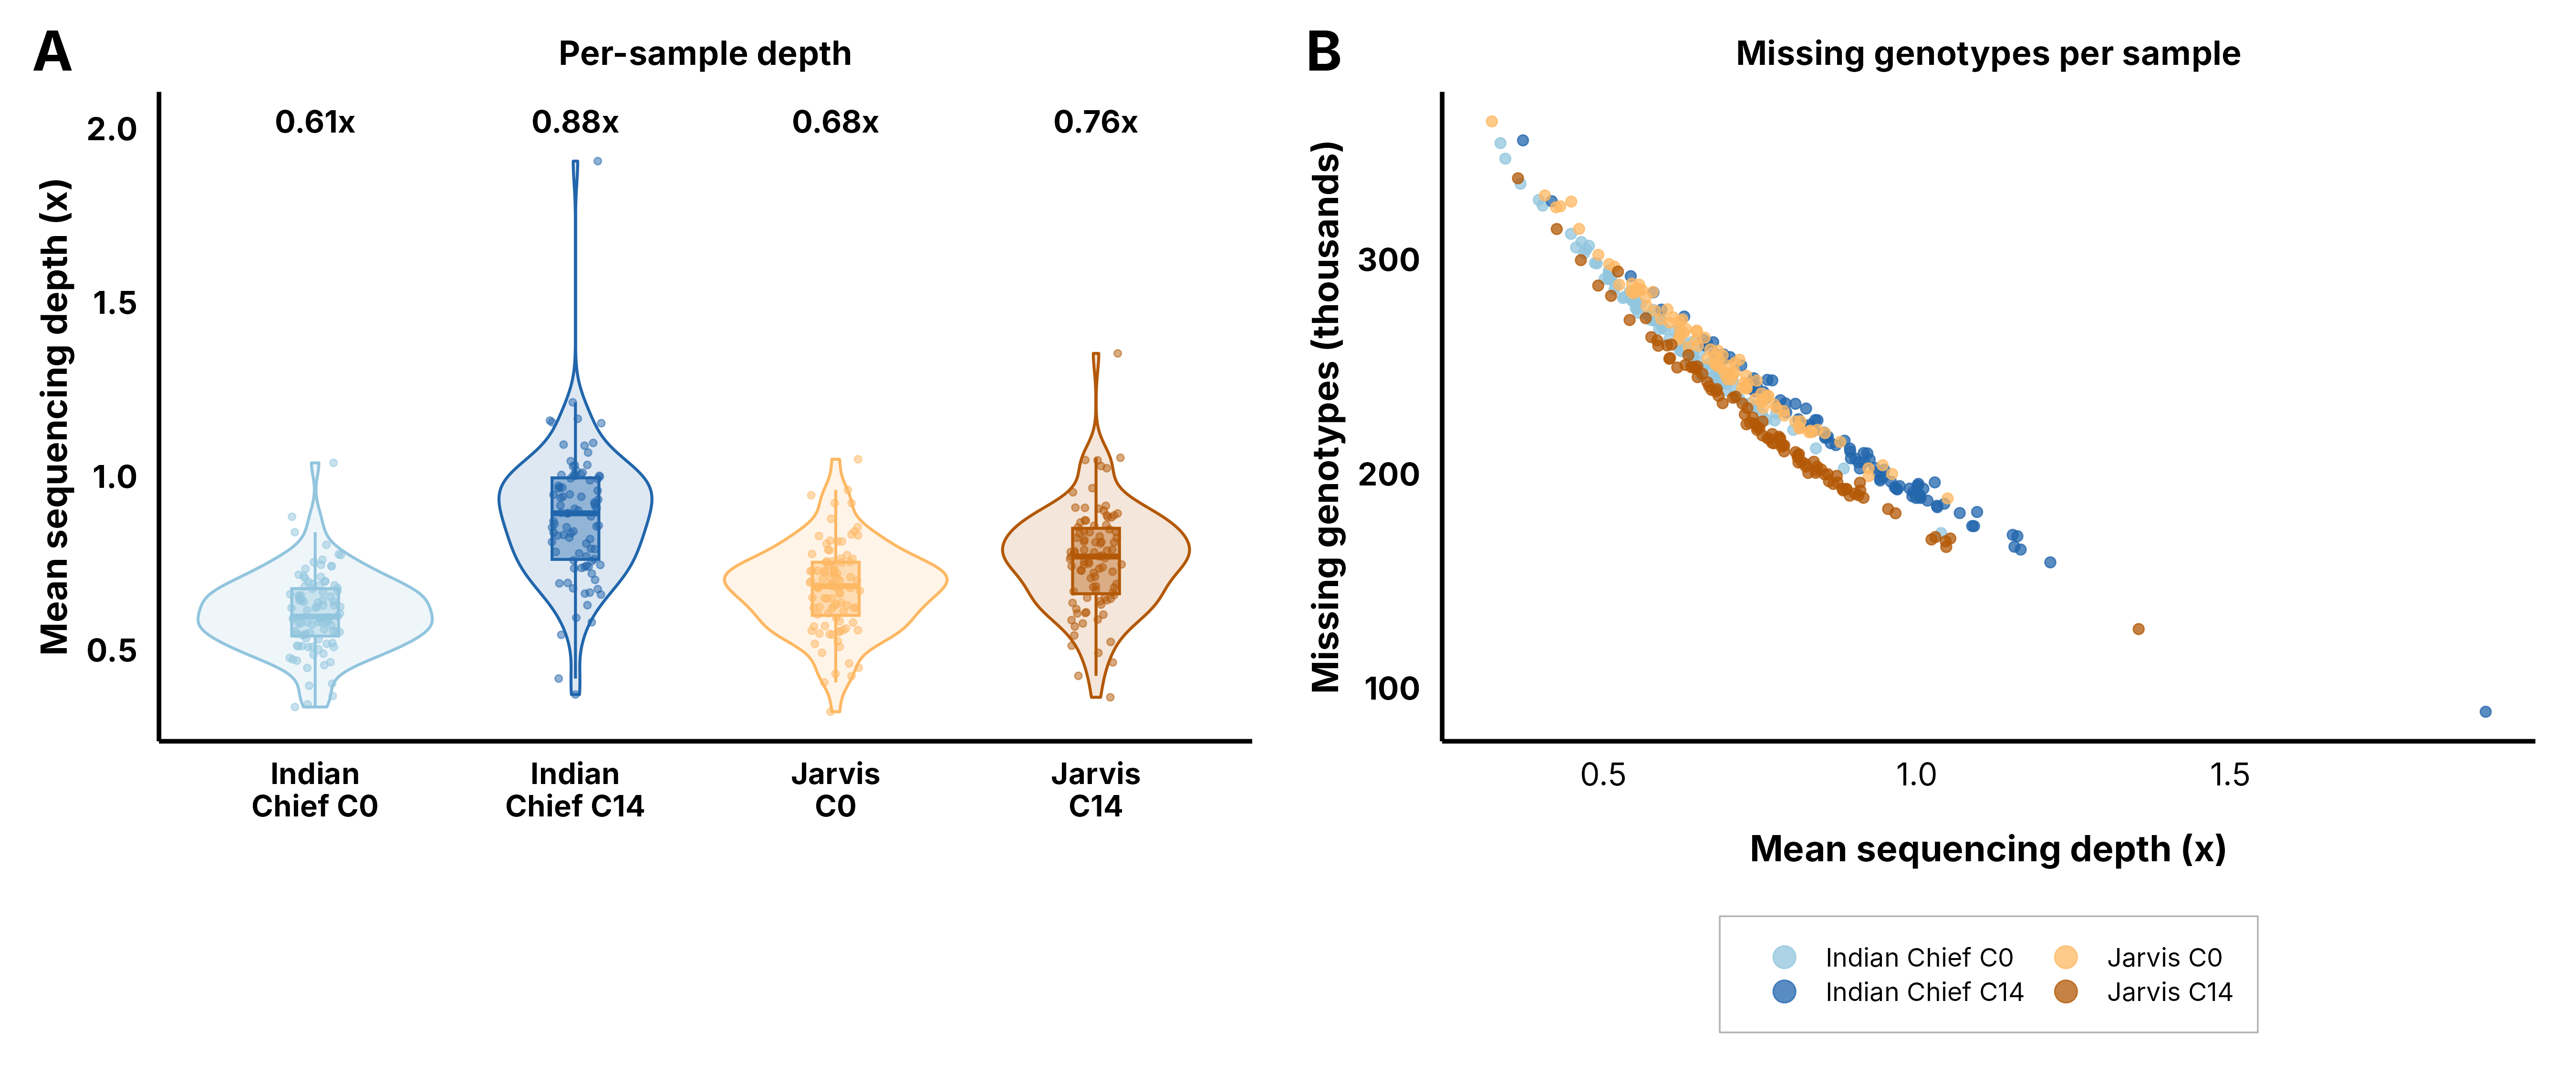
\includegraphics[width=\textwidth]{final/supp_figs/SuppFig_seq_statistics_sample_level.png}
    \caption{\textbf{Per-sample sequencing depth in the Indian Chief and Jarvis skim-sequencing data.} \textbf{(A)} Mean sequencing depth per individual for each population and cycle; numbers give group means. \textbf{(B)} Number of missing genotypes (of 512,667 filtered SNPs) per individual against its mean depth.}
    \label{fig:supp_seq_sample}
\end{figure*}



% =========================
% SUPP FIGURE S10
% =========================                                                  
\begin{figure*}[!htbp]
    \centering
    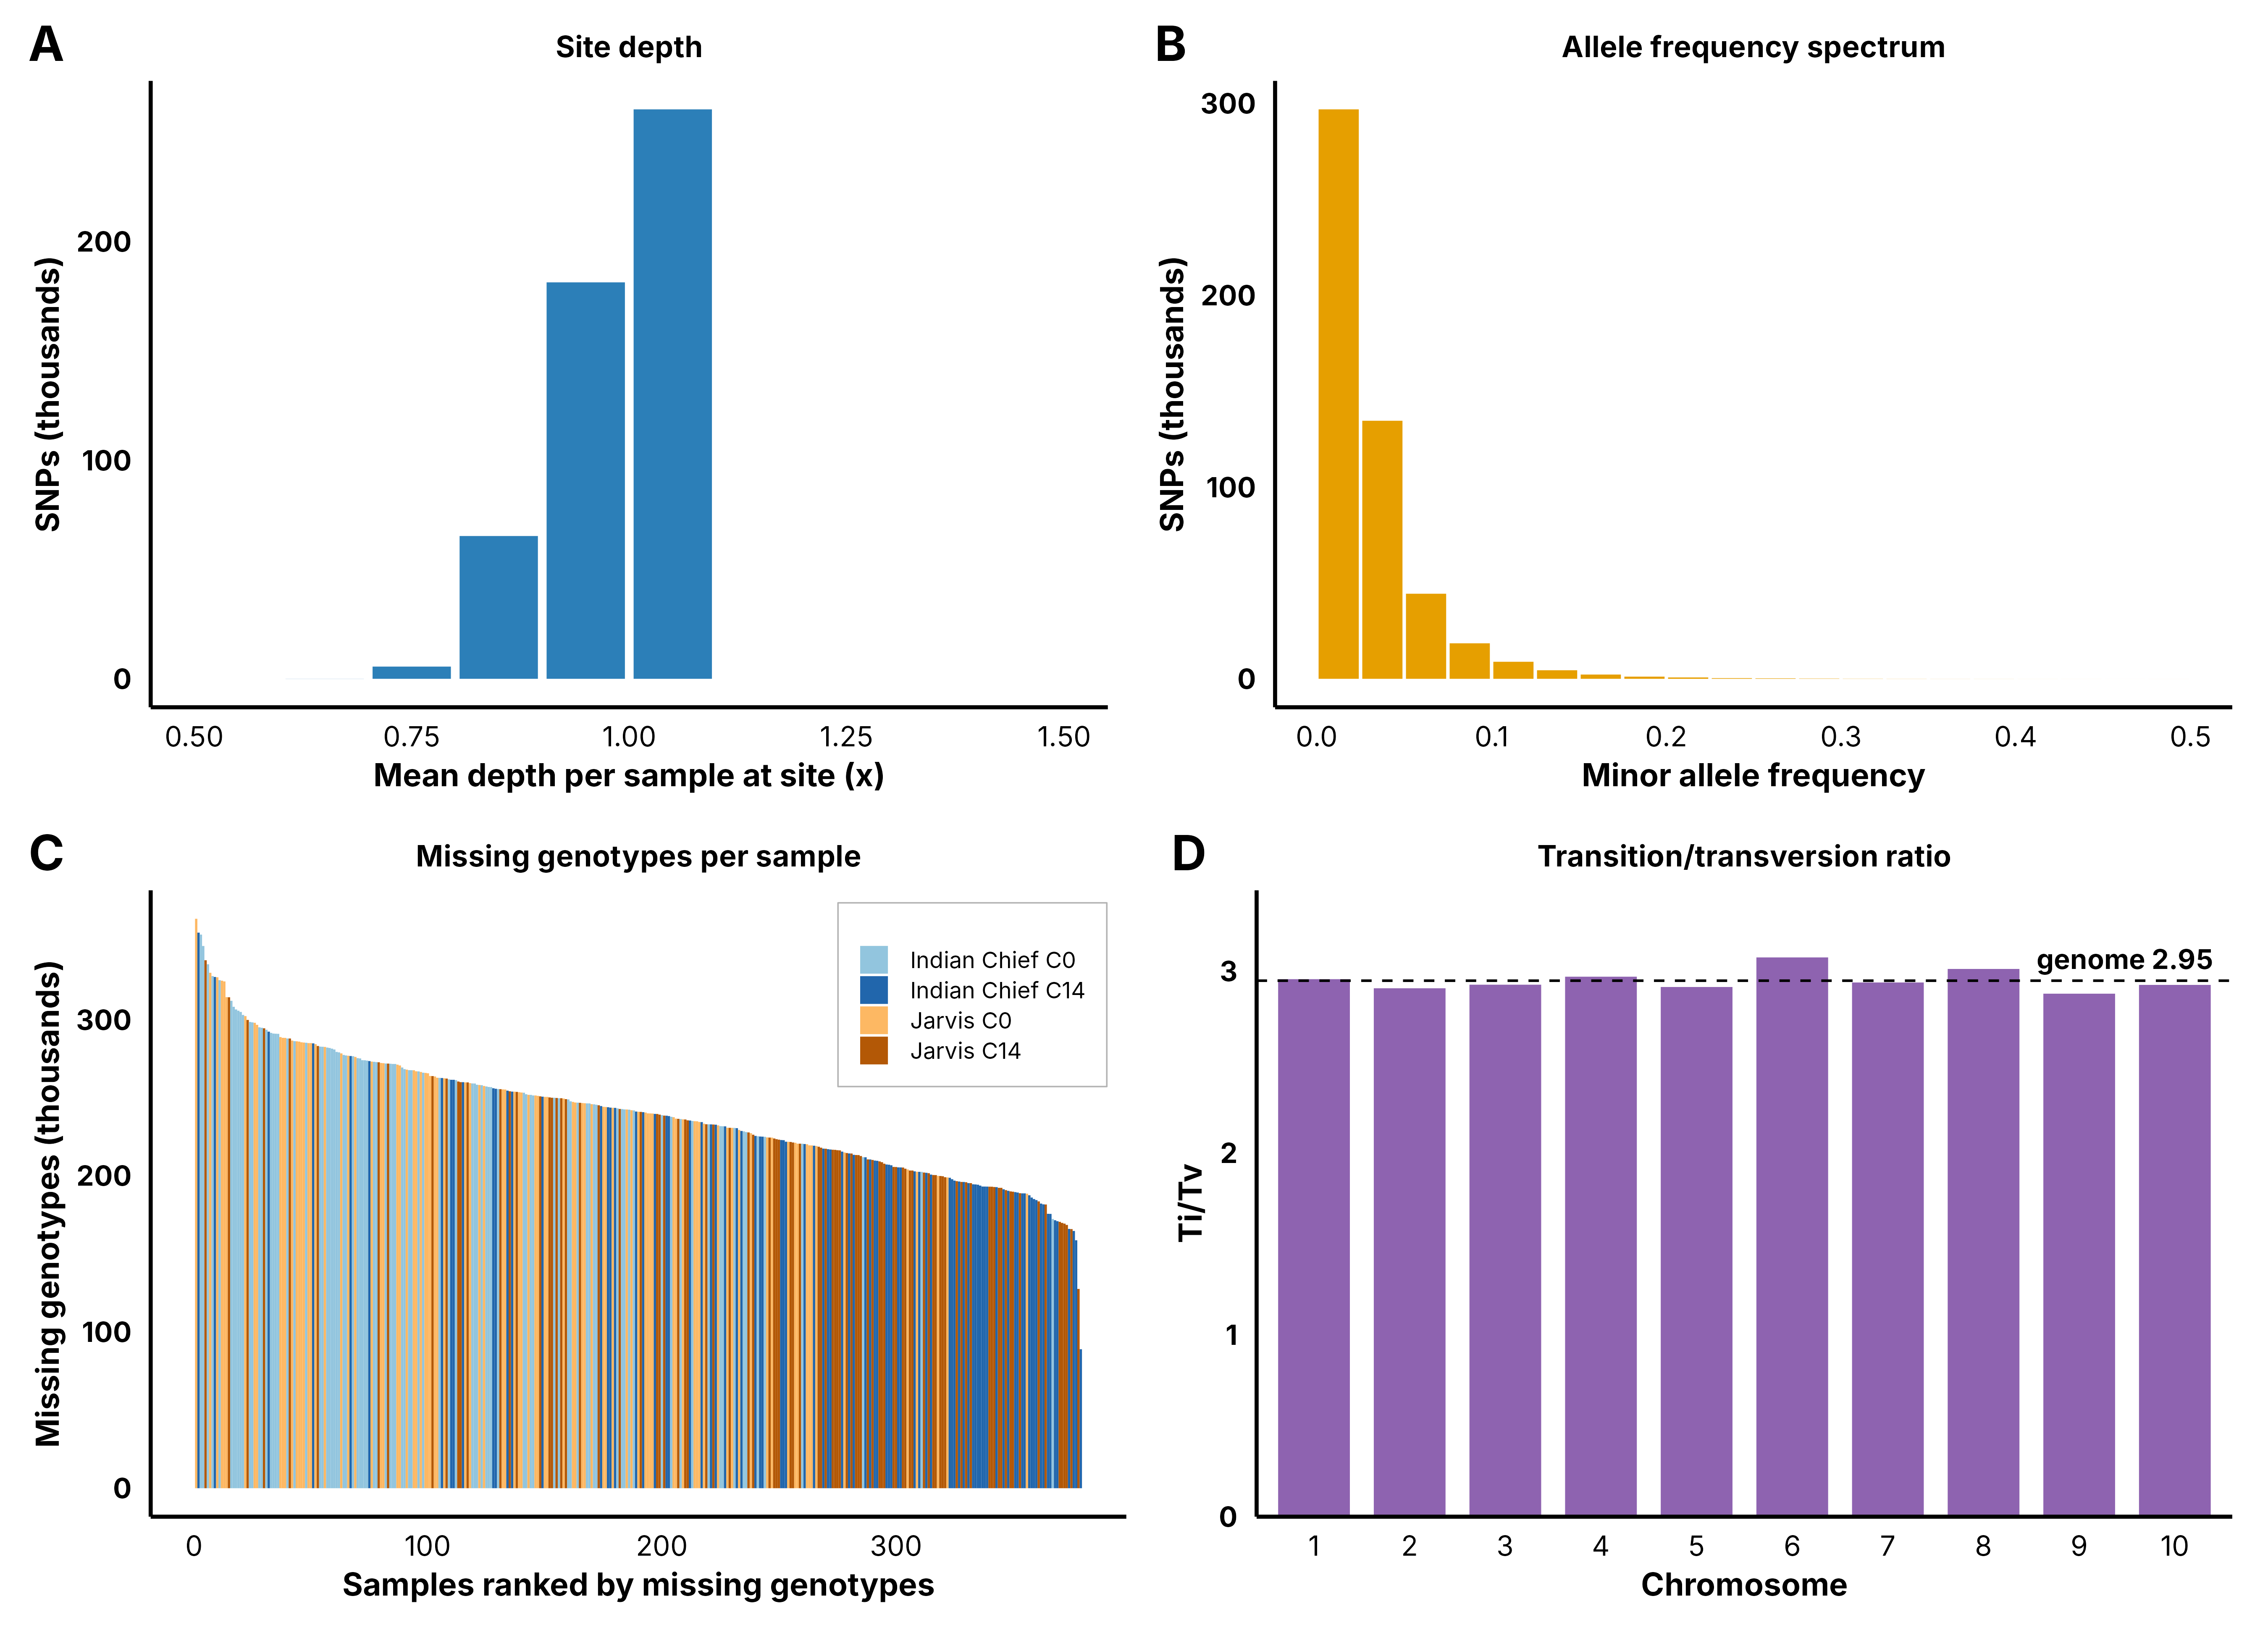
\includegraphics[width=\textwidth]{final/supp_figs/SuppFig_seq_statistics_variant_level.png}
    \caption{\textbf{Quality summaries for the 512,667 filtered SNPs.} \textbf{(A)} Mean depth per individual at each SNP (total site depth divided by 379). \textbf{(B)} Minor allele frequency spectrum, from called genotypes. \textbf{(C)} Missing genotypes per individual, ranked and coloured by population and cycle. \textbf{(D)} Transition/transversion ratio by chromosome; dashed line, genome-wide value.}
    \label{fig:supp_seq_variant}
\end{figure*}

% =========================
% SUPP FIGURE -- effective population size
% =========================
\begin{figure*}[!htbp]
    \centering
    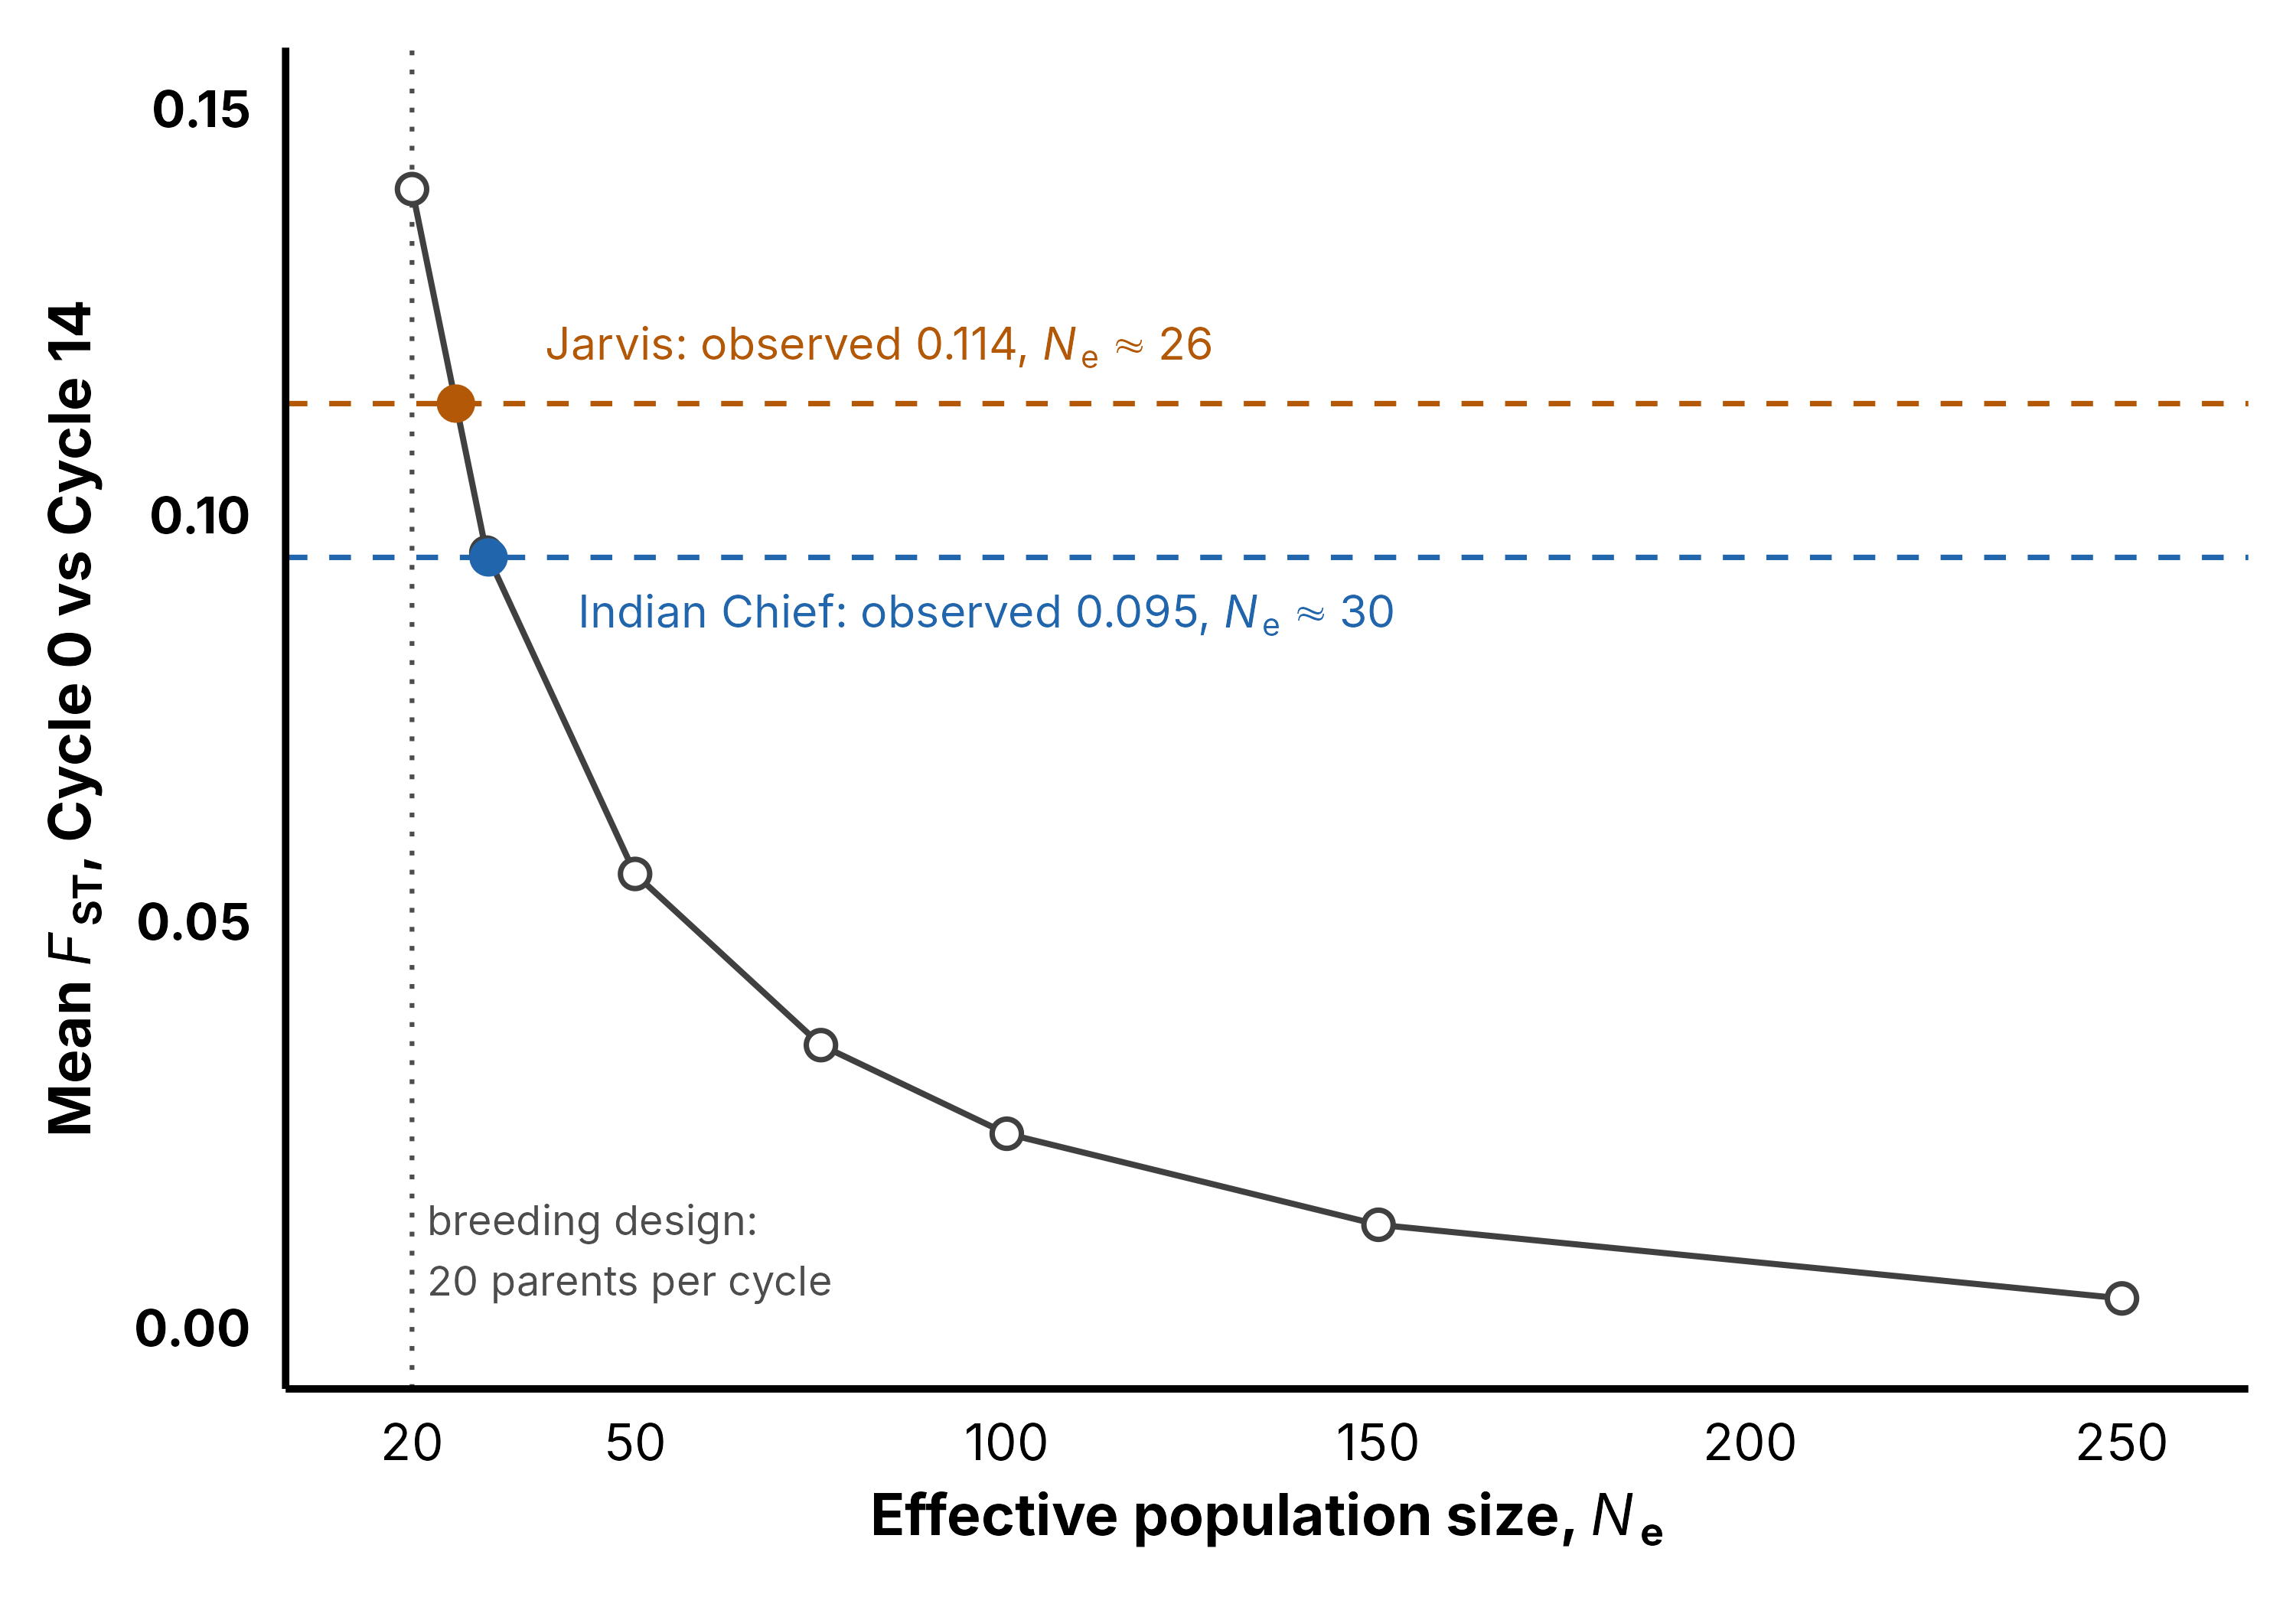
\includegraphics[width=0.75\textwidth]{final/supp_figs/SuppFig_IC_J_Ne_drift.png}
    \caption{\textbf{Effective population size of the Indian Chief and Jarvis recurrent-selection populations.} Genome-wide mean $F_{ST}$ between Cycle~0 and Cycle~14 expected under neutral Wright--Fisher drift for 14 generations across a range of effective population sizes ($N_e$; open circles), starting from the observed Cycle~0 allele frequencies and resampling the number of individuals sequenced at each site. Dashed lines give the observed values (Indian Chief 0.095, Jarvis 0.114), and filled circles mark the implied $N_e$, obtained by linear interpolation. The dotted line marks $N_e = 20$, the value expected when the 20 parents intermated in each cycle contribute equally.}
    \label{fig:supp_ne_drift}
\end{figure*}

\clearpage


% =========================
% SUPP FIGURE S9
% =========================
\begin{figure*}[!ht]
    \centering
    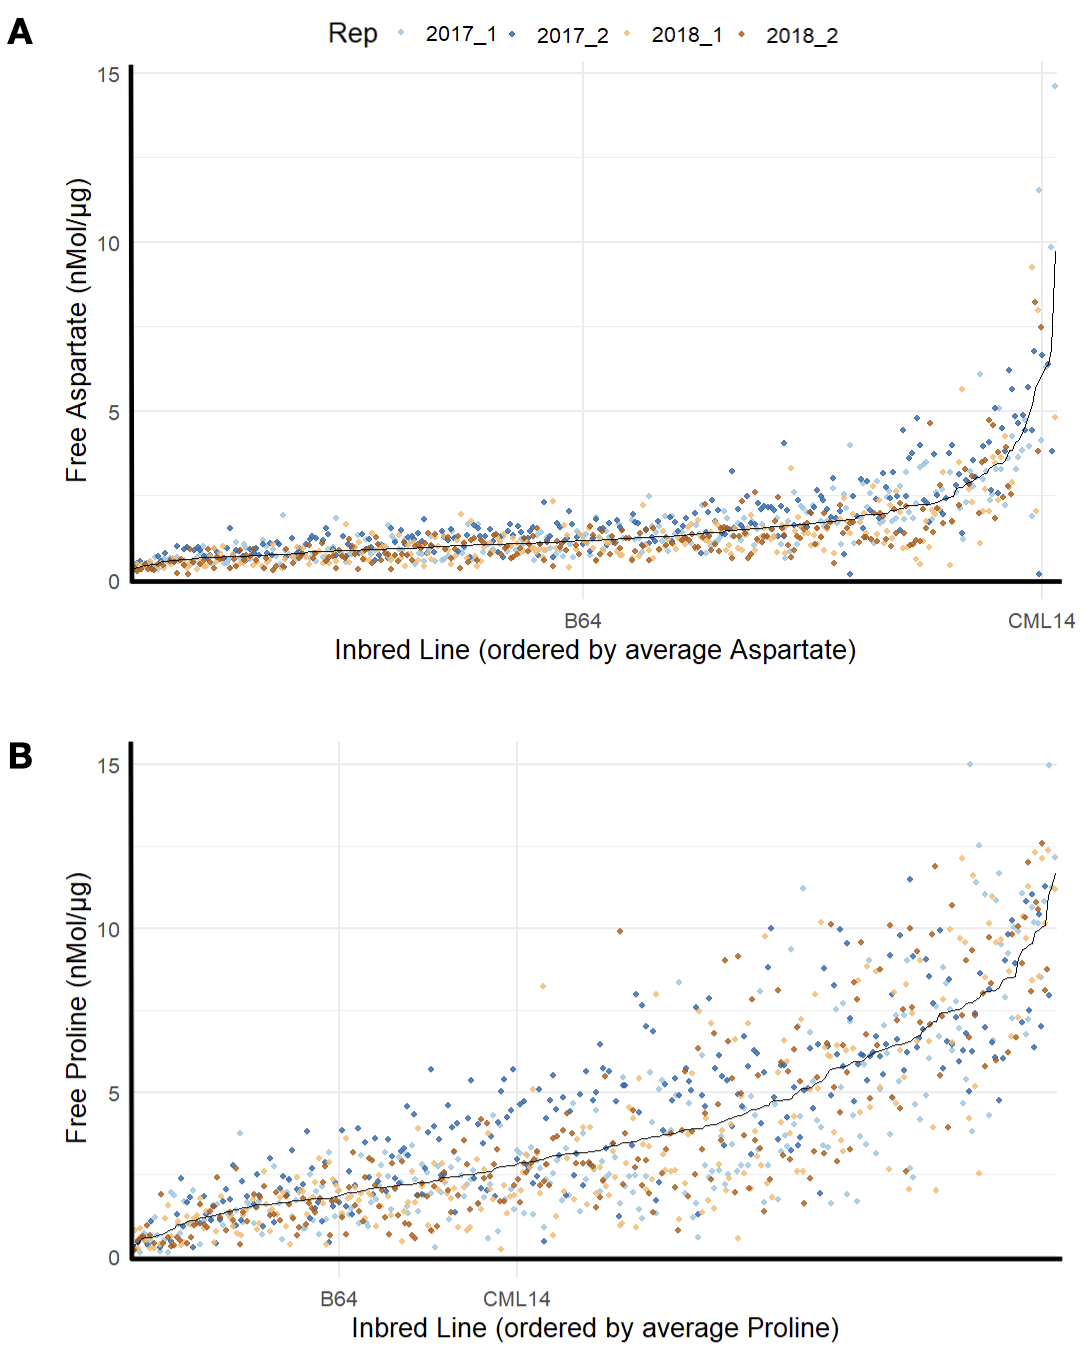
\includegraphics[width=0.85\textwidth]{Figs/Supplementary/SupFig_Asp_Pro_raw_values.png}
    \caption{\textbf{Raw free aspartate and proline variation across the Goodman--Buckler maize panel.}
    Raw amino acid measurements are shown for four replicate measurements across two years: 2017\_1, 2017\_2, 2018\_1, and 2018\_2.
    \textbf{A}, free aspartate values for inbred lines ordered by mean aspartate abundance.
    \textbf{B}, free proline values for inbred lines ordered by mean proline abundance.
    Points represent individual replicate-year measurements, and the black line shows the line-level mean across replicates.
    The parental lines B64 and CML14, used to develop the B64 $\times$ CML14 biparental population, are labeled on each panel.
    amino acid abundance is reported as nMol~$\mu$g$^{-1}$.}
    \label{fig:suppfig_asp_pro_raw_values}
\end{figure*}


% =========================
% SUPP FIGURE S10
% =========================
\begin{figure*}[!htbp]
\centering
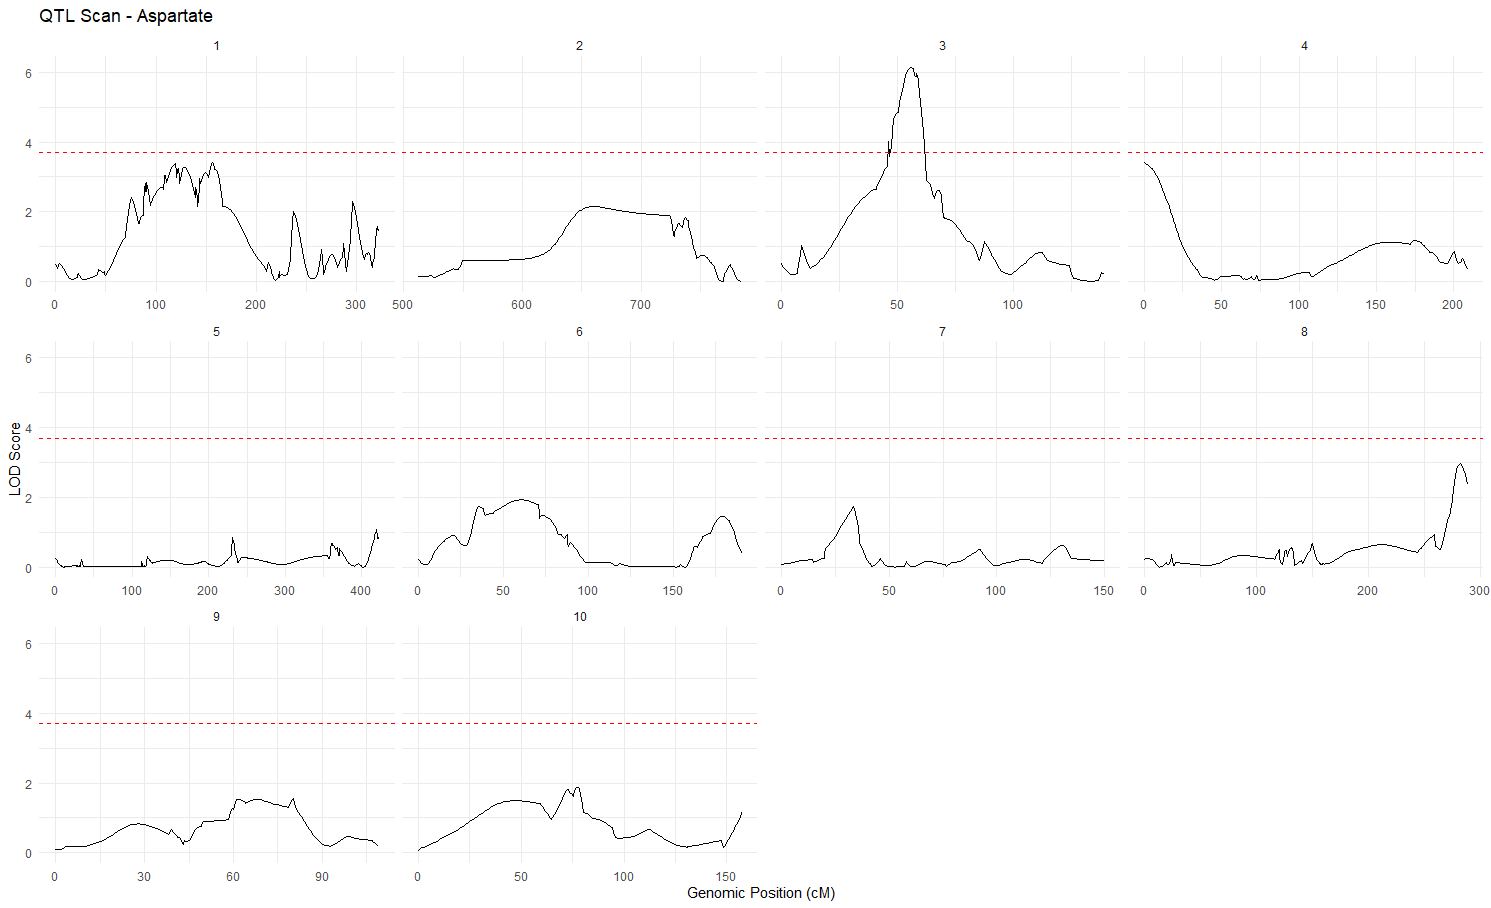
\includegraphics[width=\textwidth]{Figs/Supplementary/QTL_Aspartate.png}
\caption{
QTL for Free Aspartate. Identified from biparental F2:F3 mapping population on chromosome 3, with red dashed line representing threshold of significance.
}
\label{fig:QTL_Aspartate}
\end{figure*}

% =========================
% SUPP FIGURE S11
% =========================
\begin{figure*}[!htbp]
\centering
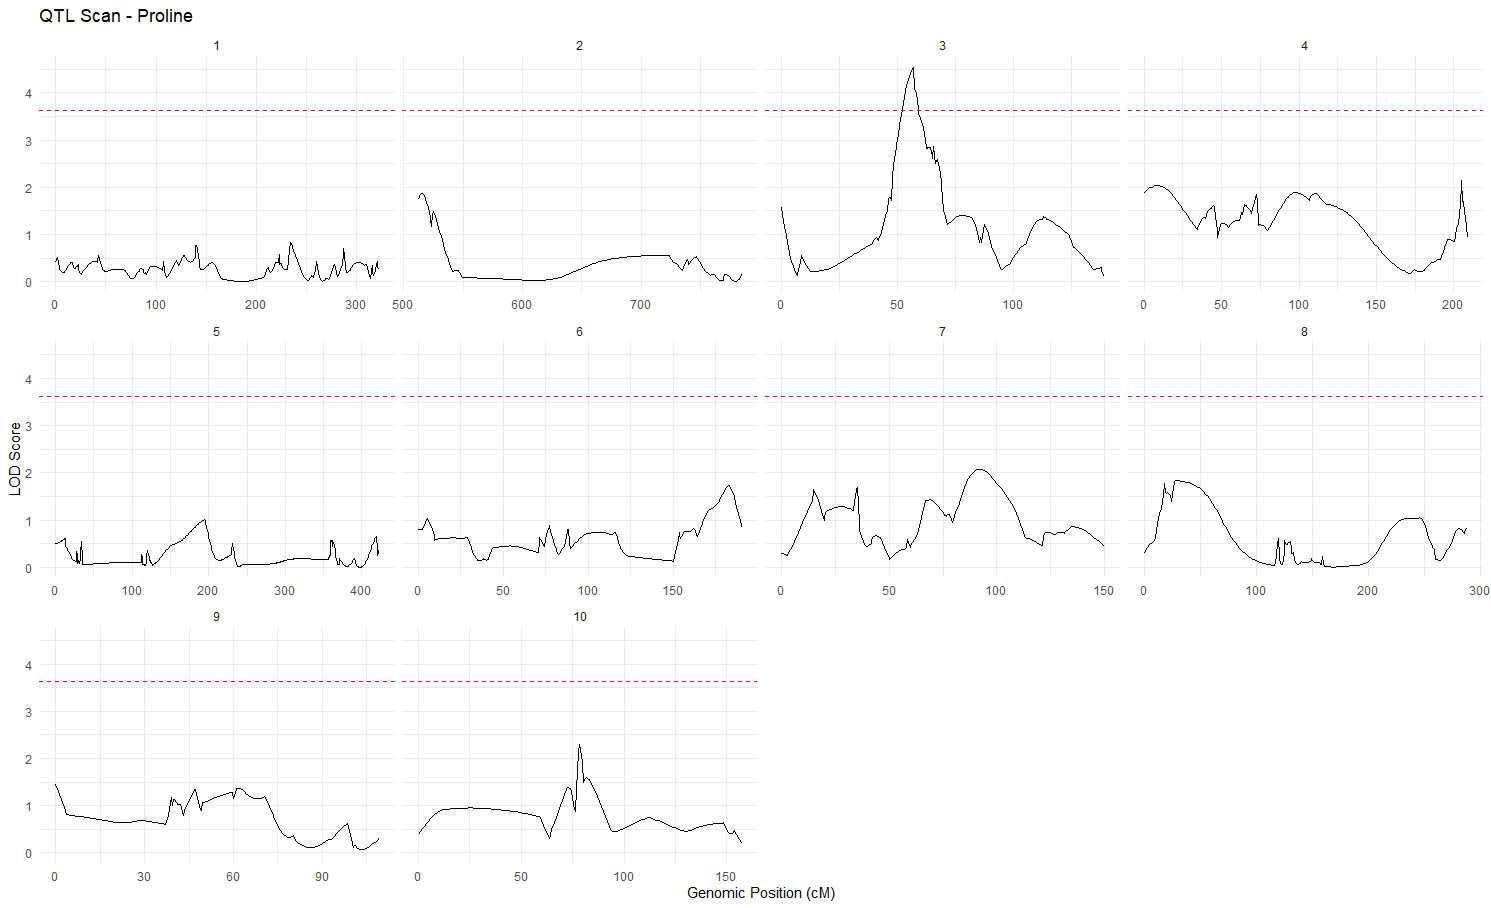
\includegraphics[width=\textwidth]{Figs/Supplementary/QTL_Proline.png}
\caption{
QTL for Free Proline. Identified from biparental F2:F3 mapping population on chromosome 3, with red dashed line representing threshold of significance.
}
\label{fig:QTL_Proline}
\end{figure*}



% =========================
% SUPP FIGURE S12
% =========================
\begin{figure*}[!htbp]
\centering
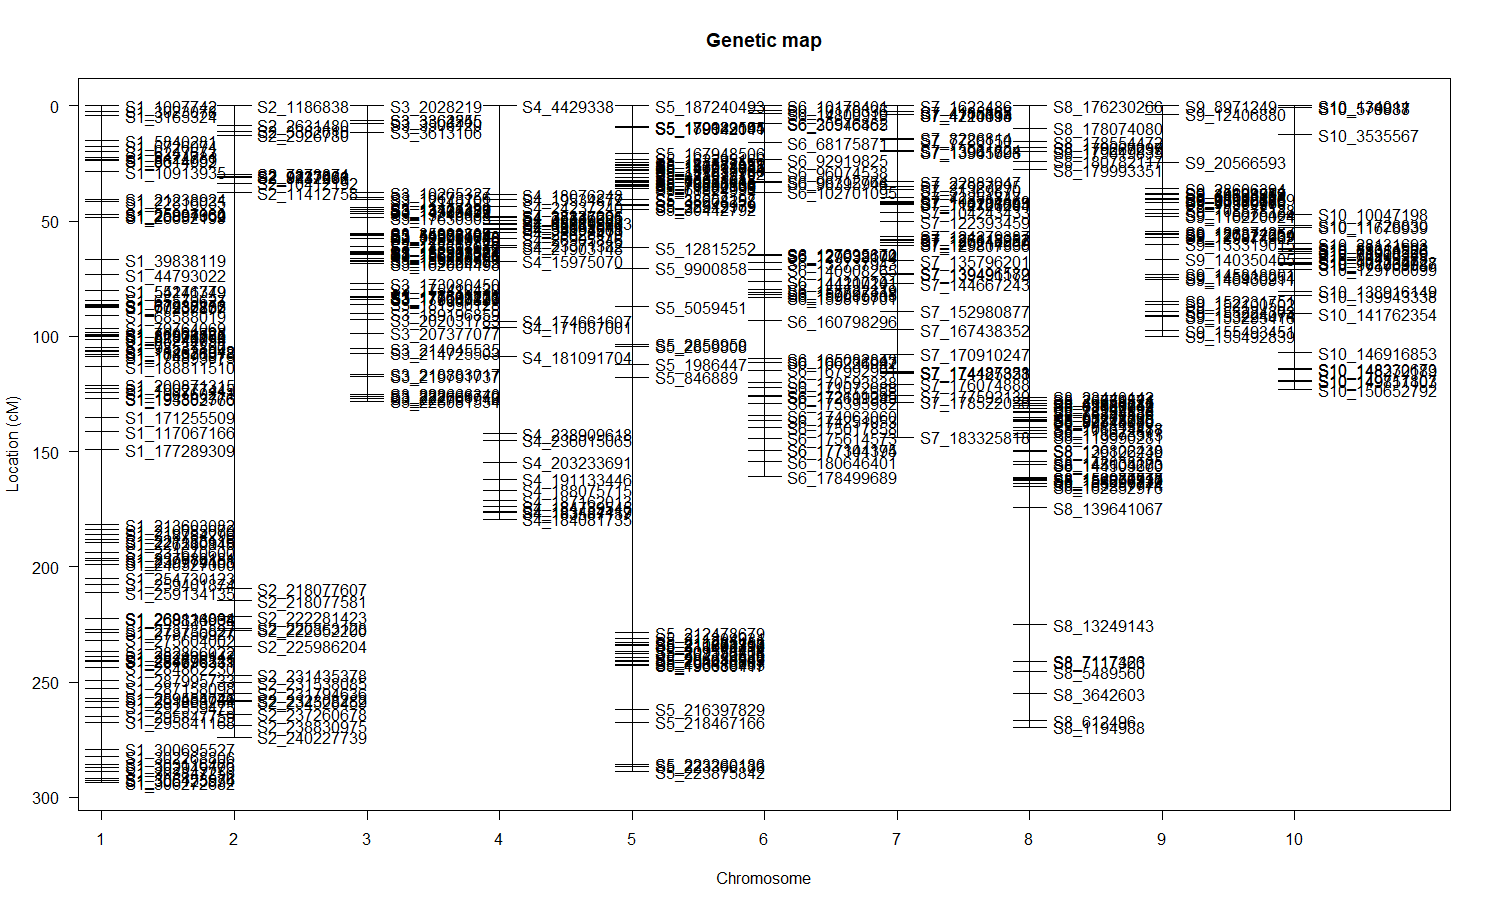
\includegraphics[width=\textwidth]{Figs/Supplementary/Nitrogen_map.png}
\caption{
Genetic map of F2:F3 mapping population
}
\label{fig:suppfig_genetic_map}
\end{figure*}


% =========================
% SUPP FIGURE S13
% =========================
\begin{figure*}[!htbp]
\centering
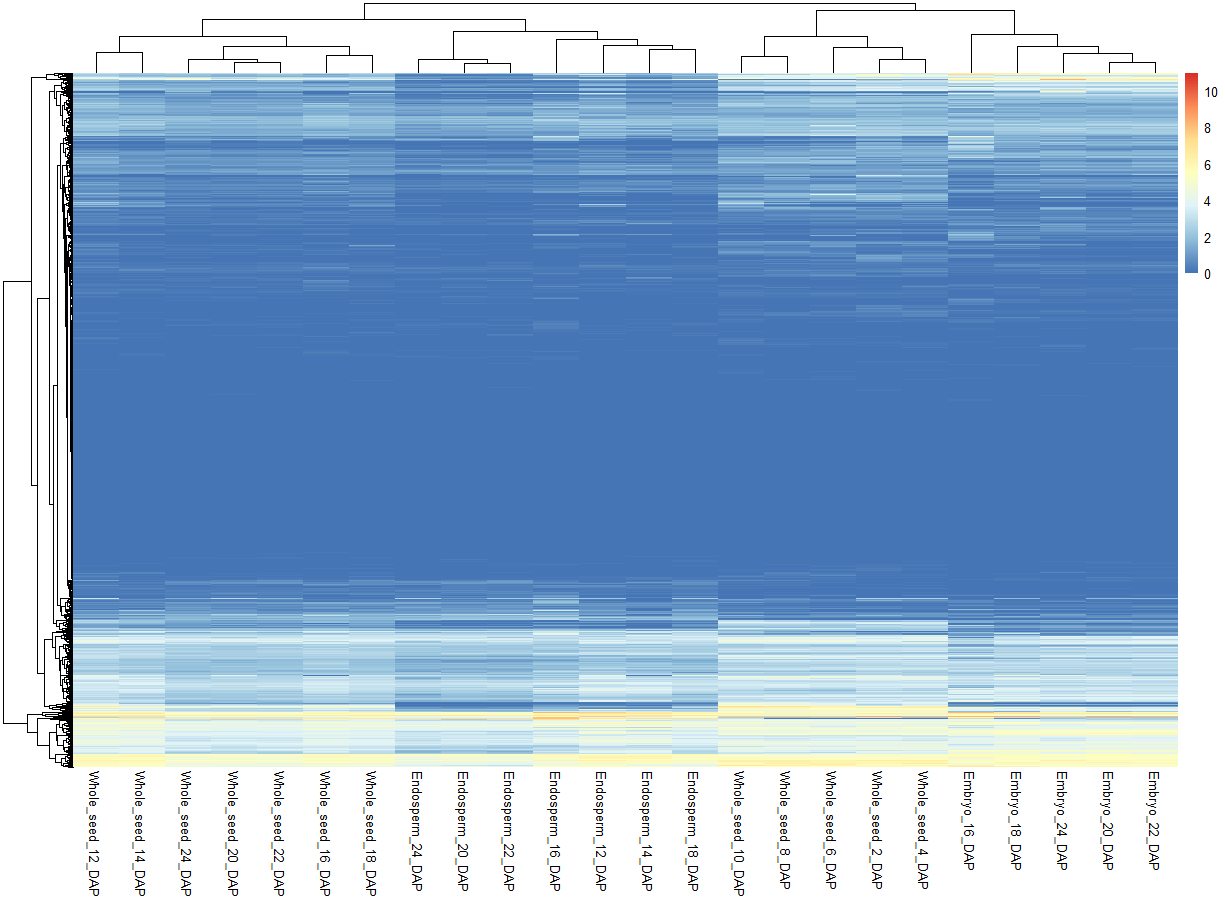
\includegraphics[width=\textwidth]{Figs/Supplementary/QTL_gene_heatmap.png}
\caption{
Heatmap showing log2-transformed expression values of genes in QTL confidence interval.
}
\label{fig:QTL_gene_heatmap}
\end{figure*}


% =========================
% SUPP FIGURE S14
% =========================


\begin{figure*}[ht!]
    \centering
    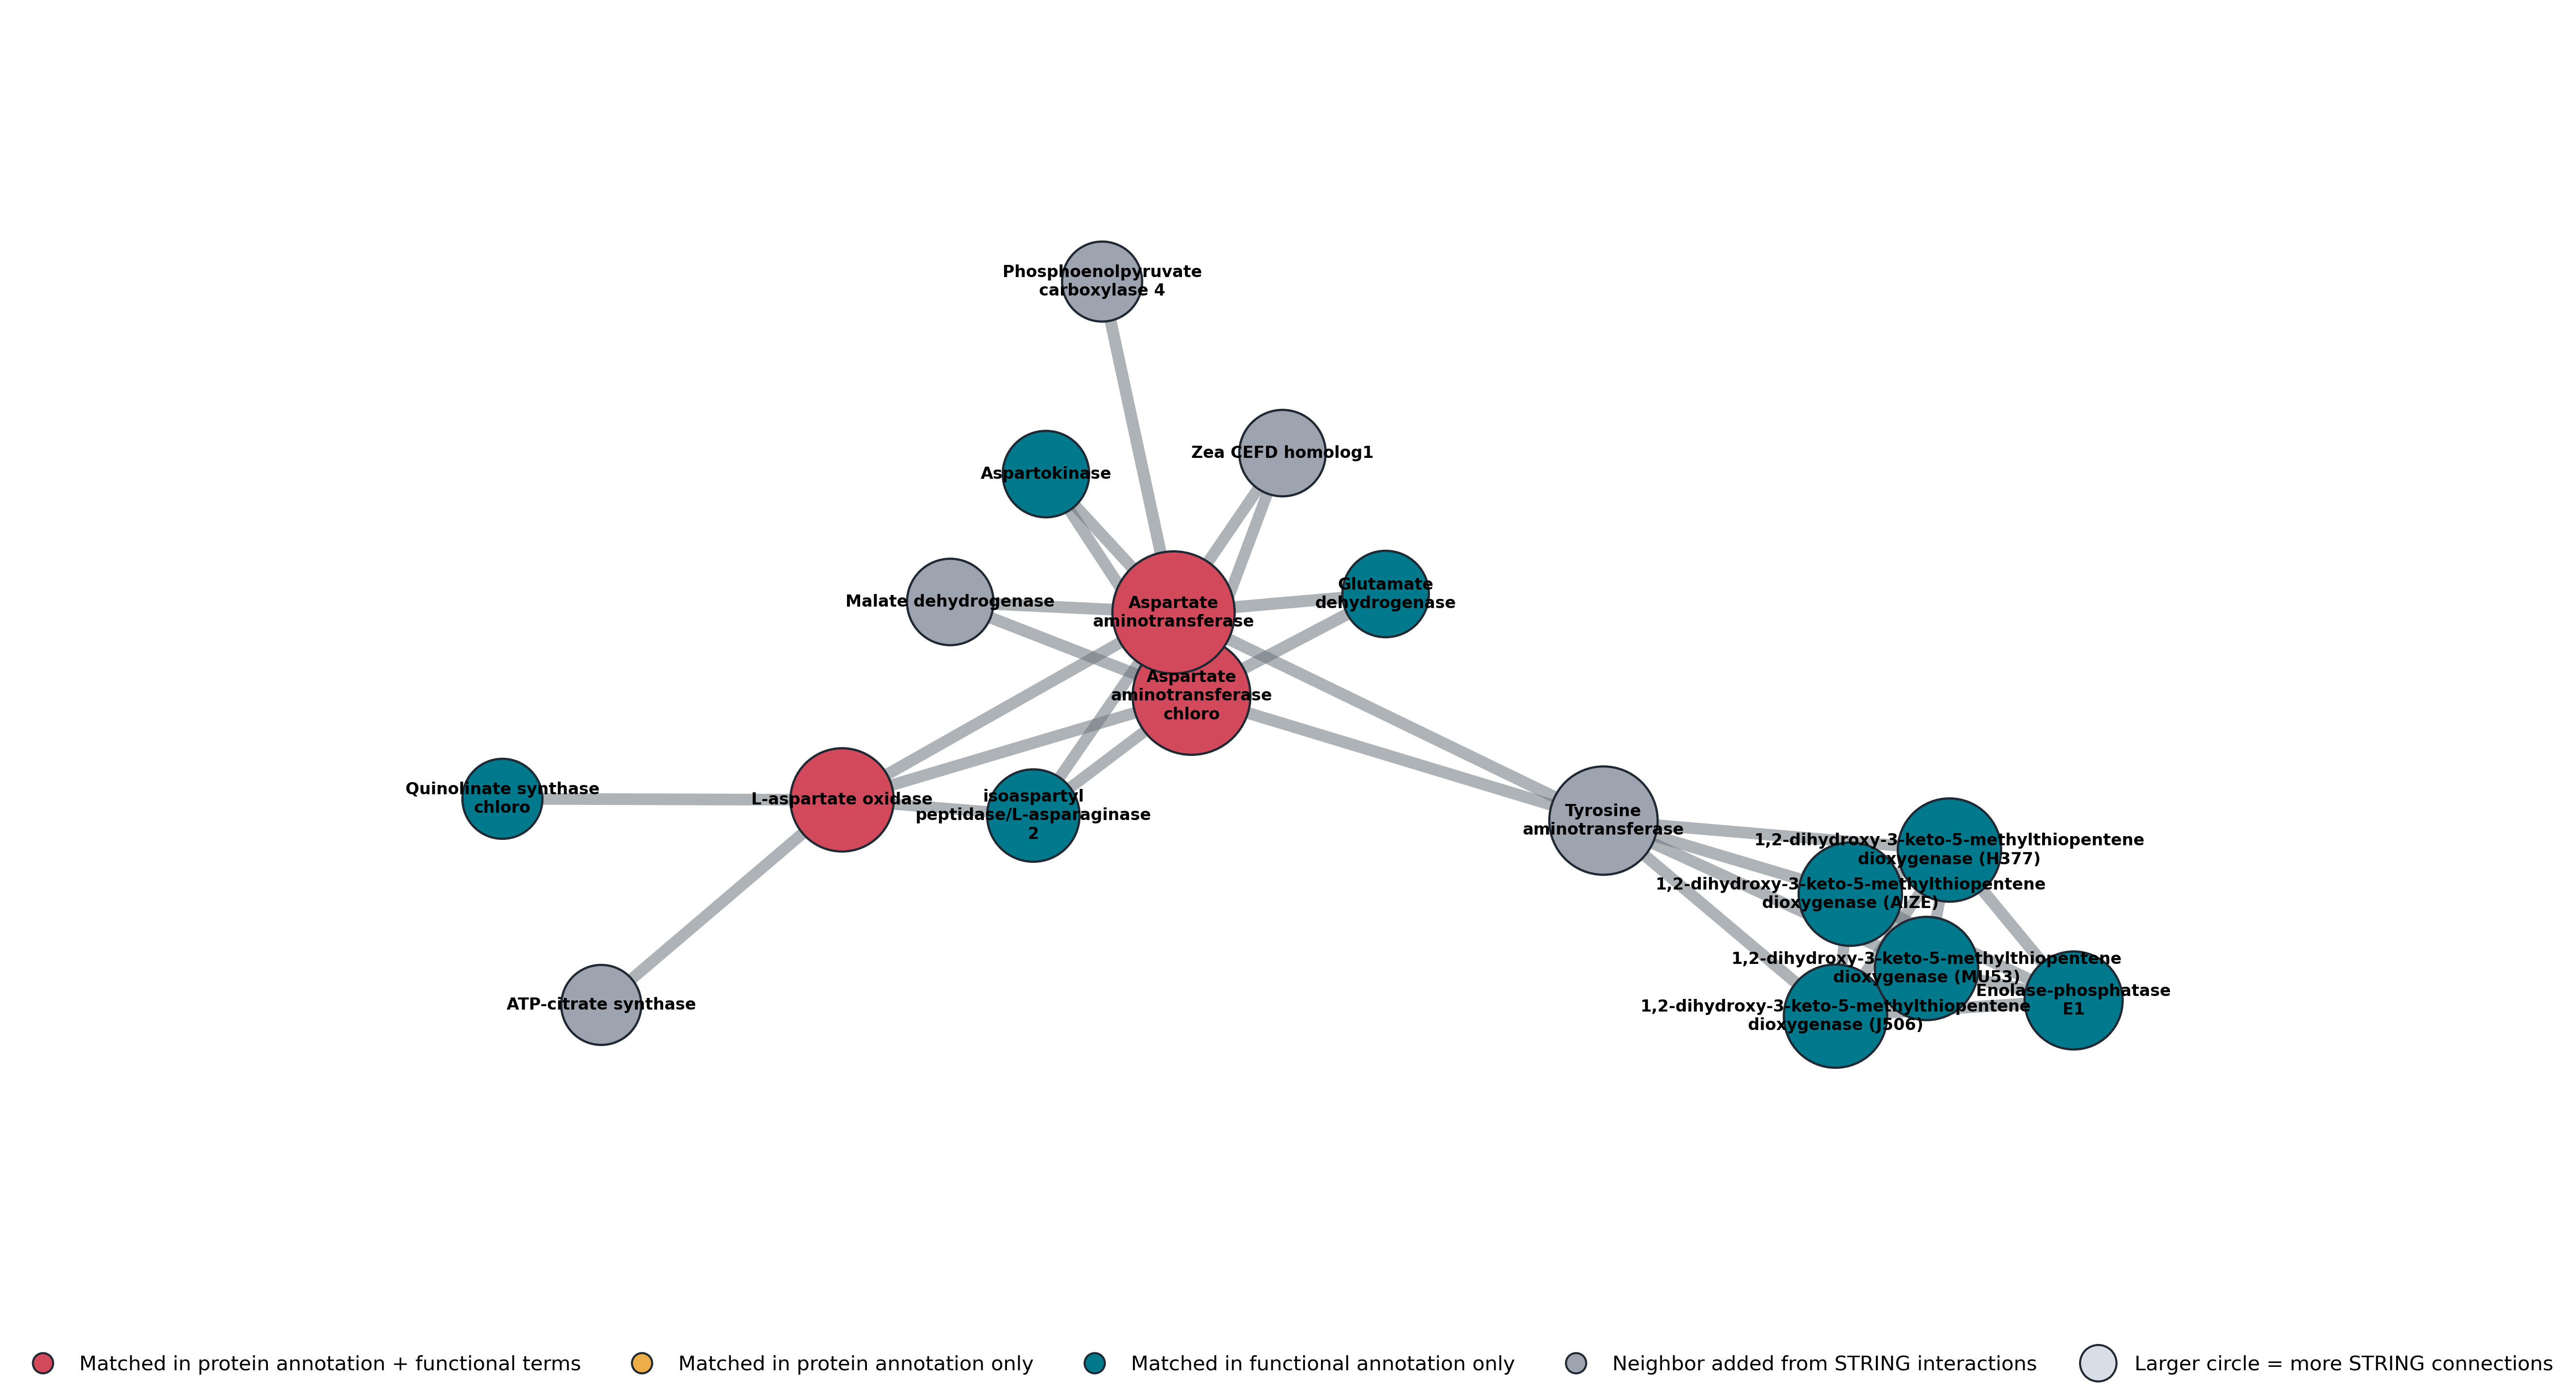
\includegraphics[width=\textwidth]{Figs/Supplementary/SuppFig_string_theme_networks.png}
    \caption{\textbf{High-confidence STRING network of candidate genes associated with maize grain nitrogen metabolism.}
    Network from STRING retaining only very high-confidence associations (combined score ≥ 0.9). Colored nodes represent candidate genes and gray nodes represent first-neighbor proteins added by STRING. Node size indicates the number of connections in the network. The network reveals a prominent aspartate/glutamate-centered module linked to nitrogen remobilization and grain nitrogen metabolism.}
    \label{fig:supp_string_theme_network}
\end{figure*}


\clearpage
\newpage

% --- Table S1 ---
\paragraph*{S1 Table.}
\phantomsection
\makeatletter
\def\@currentlabelname{S1 Table}
\makeatother
\label{S1_Table}
\textbf{Free amino acid phenotypes across the Goodman--Buckler Association Panel.} Genotype-level values of the 78 amino acid phenotypes used for GWAS for 280 of the 282 lines (two years $\times$ two blocks, Columbia, Missouri): 20 absolute FAA concentrations, six biosynthetic-family composites, 20 ratios to the total free pool, 25 ratios to the family composite, four ratios between amino acids (N.D, N.E, N.Q, Q.E) and three whole-pool traits. Trait codes are defined in Supplementary Table~S2. Provided as \texttt{SuppTable\_S1\_FAA\_phenotypes.csv}.

% --- Table S2 ---
\paragraph*{S2 Table.}
\phantomsection
\makeatletter
\def\@currentlabelname{S2 Table}
\makeatother
\label{S2_Table}
\textbf{Amino acid trait definitions.} Code and description of each of the 78 amino acid phenotypes in Supplementary Table~S1. Provided as \texttt{SuppTable\_S2\_phenotype\_definitions.csv}.

% --- Table S3 ---
\paragraph*{S3 Table.}
\phantomsection
\makeatletter
\def\@currentlabelname{S3 Table}
\makeatother
\label{S3_Table}
\textbf{Abundance, variability and heritability of the 20 free amino acids.} For each FAA across 280 lines: median, mean, standard deviation, minimum, maximum, fold range, coefficient of variation, line-mean broad-sense heritability ($H^2$) and genomic heritability ($h^2$). Provided as \texttt{SuppTable\_S3\_FAA\_abundance\_CV.csv}.

% --- Table S4 ---
\paragraph*{S4 Table.}
\phantomsection
\makeatletter
\def\@currentlabelname{S4 Table}
\makeatother
\label{S4_Table}
\textbf{Heritability of free and protein-bound amino acid traits.} Line-mean and Cullis broad-sense heritability ($H^2$) and genomic heritability ($h^2$, with 95\% interval and permuted-phenotype null) for 40 FAA and 76 PBAA traits, with sample sizes. Provided as \texttt{SuppTable\_S4\_heritability.csv}.

% --- Table S5 ---
\paragraph*{S5 Table.}
\phantomsection
\makeatletter
\def\@currentlabelname{S5 Table}
\makeatother
\label{S5_Table}
\textbf{Free vs.\ protein-bound amino acid pools.} Paired comparison of FAA and PBAA pools across matched lines for the total amino acid pool, the amino acid-derived N proxy, the proline fraction and the Asx + Glx + basic fraction (matched denominators): mean, median, standard deviation and coefficient of variation of each pool, fold difference and paired Wilcoxon $P$. Provided as \texttt{SuppTable\_S5\_FAA\_vs\_PBAA\_pools.csv}.

% --- Table S6 ---
\paragraph*{S6 Table.}
\phantomsection
\makeatletter
\def\@currentlabelname{S6 Table}
\makeatother
\label{S6_Table}
\textbf{Amino acid GWAS candidate genes.} All phenotype $\times$ SNP $\times$ gene combinations for SNPs significant at 5\% Benjamini--Hochberg FDR (per phenotype and model; MLM, BLINK, FarmCPU) within 25~kb of a B73 RefGen\_v5 gene: 1,811 SNPs, 71 phenotypes, 3,693 genes. Includes significant models, lowest $P$ and FDR, whether the SNP is significant in $\geq$2 models, gene coordinates and distance. Positions are given on AGPv4 (\texttt{Pos\_v4}, the coordinate of the genotype data) and B73 RefGen\_v5 (\texttt{Pos\_v5}, lifted with the chain file; \texttt{lift} = \texttt{gap} marks SNPs placed at the nearest aligned base); marker names carry the older AGPv3 coordinate. Provided as \texttt{SuppTable\_S6\_amino\_gwas\_candidate\_genes.csv}.

% --- Table S7 ---
\paragraph*{S7 Table.}
\phantomsection
\makeatletter
\def\@currentlabelname{S7 Table}
\makeatother
\label{S7_Table}
\textbf{Amino acid GWAS loci.} The 2,152 loci formed by merging FDR-significant SNPs within 25~kb across phenotypes, with B73 RefGen\_v5 coordinates, numbers of SNPs and phenotypes, best $P$, lead SNP (AGPv4 and v5 positions), supporting models, genes within 25~kb (or the nearest gene and its distance when none), top gene and its PANTHER family and GO terms. Provided as \texttt{SuppTable\_S7\_amino\_gwas\_loci.csv}.

% --- Table S8 ---
\paragraph*{S8 Table.}
\phantomsection
\makeatletter
\def\@currentlabelname{S8 Table}
\makeatother
\label{S8_Table}
\textbf{Soil-N GWAS candidate genes.} The 448 B73 RefGen\_v5 genes within 25~kb of the 216 soil-N SNPs (0--5~cm, 5\% FDR) that lie near a gene, one row per gene $\times$ SNP, with SNP statistics, overlap with other environmental GWAS, gene coordinates, distance, name, PANTHER family, protein class and GO terms. Provided as \texttt{SuppTable\_S8\_soilN\_candidate\_genes.csv}.

% --- Table S9 ---
\paragraph*{S9 Table.}
\phantomsection
\makeatletter
\def\@currentlabelname{S9 Table}
\makeatother
\label{S9_Table}
\textbf{Environmental GWAS overlap test.} Observed vs.\ expected numbers of shared FDR-significant SNPs (MLM, BLINK and FarmCPU combined) for each site variable against the union of geographic variables (latitude, longitude, elevation; the variable itself excluded), and for soil N (0--5~cm) against each other variable. Expected $= n_1 n_2 / M$ with $M = 495{,}755$; one-sided hypergeometric $P$, which assumes independent traits and so overstates enrichment between correlated variables. Provided as \texttt{SuppTable\_S9\_soilN\_env\_overlap\_test.csv}.

% --- Table S10 ---
\paragraph*{S10 Table.}
\phantomsection
\makeatletter
\def\@currentlabelname{S10 Table}
\makeatother
\label{S10_Table}
\textbf{Soil-N GWAS SNPs and their overlap with other environmental GWAS.} All 234 SNPs significant for soil N (0--5~cm) at 5\% FDR in MLM, BLINK or FarmCPU, with $P$ per model, MAF, number of models, whether each SNP is also FDR-significant in the GWAS of CEC, aridity, elevation, latitude, longitude, soil pH and soil N at 5--15~cm, and genes within 25~kb with the nearest gene's annotation. Provided as \texttt{SuppTable\_S10\_soilN\_SNPs\_env\_relations.csv}.

% --- Table S11 ---
\paragraph*{S11 Table.}
\phantomsection
\makeatletter
\def\@currentlabelname{S11 Table}
\makeatother
\label{S11_Table}
\textbf{Genotype--environment correlation test for soil-N SNPs.} For each of the 234 soil-N SNPs, the Pearson correlation between genotype and soil N (0--5 and 5--15~cm), latitude, longitude, elevation, soil pH, CEC and aridity across 3,107 accessions; the SNP's genome-wide rank for each variable (\% of 495,755 SNPs with a stronger correlation); the most strongly correlated non-N variable; and the call: linked to environment (top 1\% for any non-N variable), not linked, or inconclusive (weak soil-N correlation, outside the top 5\%). Provided as \texttt{SuppTable\_S11\_soilN\_geno\_env\_correlation.csv}.

% --- Table S12 ---
\paragraph*{S12 Table.}
\phantomsection
\makeatletter
\def\@currentlabelname{S12 Table}
\makeatother
\label{S12_Table}
\textbf{Expectation test for the genotype--environment correlation.} Share of SNPs in the top 1\% of the genome for at least one geographic variable (latitude, longitude, elevation) or at least one of six non-N variables (adding soil pH, CEC and aridity), for the whole genome, for SNPs in the top 1\% for correlation with soil N, for all soil-N GWAS SNPs and for those significant in $\geq$2 models, with binomial tests against the whole genome and against the soil-N-correlated SNPs. Provided as \texttt{SuppTable\_S12\_soilN\_geno\_env\_expectation.csv}.

% --- Table S13 ---
\paragraph*{S13 Table.}
\phantomsection
\makeatletter
\def\@currentlabelname{S13 Table}
\makeatother
\label{S13_Table}
\textbf{Free amino acid metrics in Indian Chief and Jarvis, Cycle~0 vs.\ Cycle~14.} Eight pre-specified FAA metrics (total FAA per mg sample; proline, asparagine, aspartate, glutamine and glutamate fractions of total FAA; Asn + Gln + Arg + Lys + His per mg; FAA-derived N per mg) per population: biological-sample sizes, means and medians per cycle, two-sided Wilcoxon rank-sum $P$, Benjamini--Hochberg-adjusted $P$ across the eight metrics, Cliff's $\delta$ (C14 vs.\ C0) and direction of change. Provided as \texttt{SuppTable\_S13\_IC\_J\_FAA\_metrics.csv}.

% --- Table S14 ---
\paragraph*{S14 Table.}
\phantomsection
\makeatletter
\def\@currentlabelname{S14 Table}
\makeatother
\label{S14_Table}
\textbf{Amino acid composition in Indian Chief and Jarvis, Cycle~0 vs.\ Cycle~14.} For each of the 20 free and 16 protein-bound amino acids, its fraction of the total pool per population and cycle: sample sizes, means, medians, Wilcoxon rank-sum $P$, Benjamini--Hochberg-adjusted $P$ across the amino acids of that pool, Cliff's $\delta$ and direction of change. Provided as \texttt{SuppTable\_S14\_IC\_J\_amino\_acid\_composition.csv}.

% --- Table S15 ---
\paragraph*{S15 Table.}
\phantomsection
\makeatletter
\def\@currentlabelname{S15 Table}
\makeatother
\label{S15_Table}
\textbf{Protein-bound amino acid metrics in Indian Chief and Jarvis, Cycle~0 vs.\ Cycle~14.} Six PBAA metrics (total PBAA per mg sample; proline, Asx and Glx fractions; Asx + Glx + Arg + Lys + His per mg; estimated PBAA-derived N per mg, with Asx and Glx at 1.5 N), with the same statistics as Supplementary Table~S13 and Benjamini--Hochberg adjustment across the six. Provided as \texttt{SuppTable\_S15\_IC\_J\_PBAA\_metrics.csv}.

% --- Table S16 ---
\paragraph*{S16 Table.}
\phantomsection
\makeatletter
\def\@currentlabelname{S16 Table}
\makeatother
\label{S16_Table}
\textbf{Amino acid-derived nitrogen per mg sample in Indian Chief and Jarvis.} FAA-derived N, estimated PBAA-derived N and estimated total amino acid-derived N per mg sample, per population and cycle, with Wilcoxon rank-sum $P$ and Benjamini--Hochberg-adjusted $P$ across the three measures. Provided as \texttt{SuppTable\_S16\_IC\_J\_AA\_N\_per\_mg.csv}.

% --- Table S17 ---
\paragraph*{S17 Table.}
\phantomsection
\makeatletter
\def\@currentlabelname{S17 Table}
\makeatother
\label{S17_Table}
\textbf{Indian Chief $F_{ST}$ windows, Cycle~0 vs.\ Cycle~14.} All 2,162 GenWin spline windows with chromosome, window number, start and end (B73 RefGen\_v5), number of sites, mean per-site $F_{ST}$, whether the window is in the top 5\% ($F_{ST} \geq 0.157$), and the number and IDs of overlapping genes. Provided as \texttt{SuppTable\_S17\_IC\_Fst\_windows.csv}.

% --- Table S18 ---
\paragraph*{S18 Table.}
\phantomsection
\makeatletter
\def\@currentlabelname{S18 Table}
\makeatother
\label{S18_Table}
\textbf{Jarvis $F_{ST}$ windows, Cycle~0 vs.\ Cycle~14.} All 2,151 GenWin spline windows, with the same columns as Supplementary Table~S17 (top 5\%: $F_{ST} \geq 0.178$). Provided as \texttt{SuppTable\_S18\_J\_Fst\_windows.csv}.

% --- Table S19 ---
\paragraph*{S19 Table.}
\phantomsection
\makeatletter
\def\@currentlabelname{S19 Table}
\makeatother
\label{S19_Table}
\textbf{Indian Chief candidate genes in top-5\% $F_{ST}$ windows.} The 2,001 genes overlapping the 109 top-5\% windows, with gene name, window coordinates and $F_{ST}$, whether the gene also lies in a top-5\% Jarvis window (\texttt{shared\_with\_other\_population}), PANTHER family and protein class, and Gene Ontology molecular function, biological process, and cellular component terms. Genes in the same window share one $F_{ST}$ value and are not independent. Provided as \texttt{SuppTable\_S19\_IC\_Fst\_top5\_genes.csv}.

% --- Table S20 ---
\paragraph*{S20 Table.}
\phantomsection
\makeatletter
\def\@currentlabelname{S20 Table}
\makeatother
\label{S20_Table}
\textbf{Jarvis candidate genes in top-5\% $F_{ST}$ windows.} The 1,179 genes overlapping the 108 top-5\% windows, with the same columns as Supplementary Table~S19. Provided as \texttt{SuppTable\_S20\_J\_Fst\_top5\_genes.csv}.

% --- Table S22 ---
\paragraph*{S22 Table.}
\phantomsection
\makeatletter
\def\@currentlabelname{S22 Table}
\makeatother
\label{S22_Table}
\textbf{Genotype-level FAA and PBAA means across the Goodman--Buckler Association Panel.} Mean free amino acid (FAA) and protein-bound amino acid (PBAA) values for matched Goodman--Buckler taxa, together with derived metrics including total FAA, total PBAA, proline fractions, nitrogen-rich fractions, and amino-acid-derived nitrogen proxy values calculated on the source assay scale.

% --- Table S23 ---
\paragraph*{S23 Table.}
\phantomsection
\makeatletter
\def\@currentlabelname{S23 Table}
\makeatother
\label{S23_Table}
\textbf{Summary statistics for FAA and PBAA metrics across the Goodman--Buckler Association Panel.} Mean, median, standard deviation, minimum, maximum, and sample size for genotype-level FAA, PBAA, and derived amino-acid nitrogen proxy metrics across matched Goodman--Buckler taxa.

% --- Table S24 ---
\paragraph*{S24 Table.}
\phantomsection
\makeatletter
\def\@currentlabelname{S24 Table}
\makeatother
\label{S24_Table}
\textbf{Paired comparisons of FAA and PBAA metrics across the Goodman--Buckler Association Panel.} Paired Wilcoxon signed-rank test results comparing FAA and PBAA values across matched Goodman--Buckler taxa for broad amino acid pool size, amino-acid-derived nitrogen proxy, proline fraction, and nitrogen-rich fraction.

% --- Table S25 ---
\paragraph*{S25 Table.}
\phantomsection
\makeatletter
\def\@currentlabelname{S25 Table}
\makeatother
\label{S25_Table}
\textbf{Candidate genes within the Pro/Asp QTL region with embryo RNA-seq expression.} RNA-seq expression values are shown for candidate genes in the chromosome~3 Pro/Asp QTL region across maize embryo developmental stages at 16, 18, 20, and 22 days after pollination (DAP). The table includes gene identifier, chromosome, genomic start position, gene annotation, and embryo-stage expression values. The full table is provided as \texttt{SuppTable\_25\_QTL\_genes\_RNAseq\_embryo}.


\end{document}
